\documentclass[compress,red]{beamer}
\usepackage{etex}
\mode<presentation>

\usetheme{Warsaw}
%\usetheme{Madrid}

\setbeamertemplate{navigation symbols}{}
\setbeamertemplate{headline}{}

%\setbeameroption{show notes}
%\setbeameroption{show only notes}
\setbeameroption{hide notes}

%\hypersetup{pdfpagemode=FullScreen} % makes your presentation go automatically to full screen
%\useoutertheme[subsection=false]{smoothbars}
\useoutertheme{shadow}

% include packages
\usepackage{subfigure}
\usepackage{textcomp}
\usepackage{multicol}
\usepackage{amsmath}
\usepackage{epsfig}
\usepackage{graphicx}
\usepackage[all,knot]{xy}
\xyoption{arc}
\usepackage{url}
\usepackage{multimedia}
\usepackage{hyperref}
\usepackage{helvet}
\usepackage[english]{babel}
\usepackage[utf8]{inputenc}
\usepackage{multirow}
\usepackage{verbatim}
%\usepackage{geometry}
%\geometry{verbose,letterpaper}
%\usepackage{movie15}
%\usepackage{hyperref}
\usepackage{pgfpages}
\usepackage{setspace}


\graphicspath{{../pictures/}}

%\logo{}
\titlegraphic{\scalebox{4}{
    
\includegraphics[height=0.5cm]{ohwr_logo.eps}
  }
}


%\title{F*WATCH, making a watch differently!}
\title[{\makebox[.45\paperwidth]{F*WATCH\hfill%
       \insertframenumber/\inserttotalframenumber}}]{F*WATCH, making a watch differently!}


\author % (optional, use only with lots of authors)
{Federico Vaga, Matthieu Cattin}
% - Give the names in the same order as the appear in the paper.
% - Use the \inst{?} command only if the authors have different
%   affiliation.

%\institute%[Universities of Somewhere and Elsewhere] % (optional, but mostly needed)
%{
  %\inst{1}%
  %BE-CO Hardware and Timing section\\
  %CERN, Geneva, Switzerland
 %\and
 %\inst{2}%
 %Department of Theoretical Philosophy\\
 %University of Elsewhere
% }
% - Use the \inst command only if there are several affiliations.
% - Keep it simple, no one is interested in your street address.

\date %(optional, should be abbreviation of conference name)
{FOSDEM, Brussels, 31 January 2015}
% - Either use conference name or its abbreviation.
% - Not really informative to the audience, more for people (including
%   yourself) who are reading the slides online

%\subject{Theoretical Computer Science}
% This is only inserted into the PDF information catalog. Can be left
% out.


% If you have a file called "university-logo-filename.xxx", where xxx
% is a graphic format that can be processed by latex or pdflatex,
% resp., then you can add a logo as follows:

%\pgfdeclareimage[height=1cm]{ohr-logo}{ohr_logo.jpg}
%\logo{\pgfuseimage{ohr-logo}}


% Delete this, if you do not want the table of contents to pop up at
% the beginning of each subsection:
%\AtBeginSection[]
%{
%  \begin{frame}<beamer>{Outline}
%    \tableofcontents[currentsection]
%  \end{frame}
%}


% If you wish to uncover everything in a step-wise fashion, uncomment
% the following command:

%\beamerdefaultoverlayspecification{<+->}

\begin{document}

\begin{frame}
  \titlepage
  \note[item]{Federico: software engineer}
  \note[item]{Matthieu: electronic engineer}
  \note[item]{CERN BE-CO}.
  \note[item]{free time project}
\end{frame}

%\begin{frame}{Outline}
%  \tableofcontents
  % You might wish to add the option [pausesections]
%\end{frame}


% Structuring a talk is a difficult task and the following structure
% may not be suitable. Here are some rules that apply for this
% solution:

% - Exactly two or three sections (other than the summary).
% - At *most* three subsections per section.
% - Talk about 30s to 2min per frame. So there should be between about
%   15 and 30 frames, all told.

% - A conference audience is likely to know very little of what you
%   are going to talk about. So *simplify*!
% - In a 20min talk, getting the main ideas across is hard
%   enough. Leave out details, even if it means being less precise than
%   you think necessary.
% - If you omit details that are vital to the proof/implementation,
%   just say so once. Everybody will be happy with that.



%#####################################################################
%############ SECTION ################################################
\section{Introduction}

\subsection*{} % dummy subsection to display dots

%------------ FRAME --------------------------------------------------
\begin{frame}{What is it?}
  \begin{center}
      \alt<2> {
        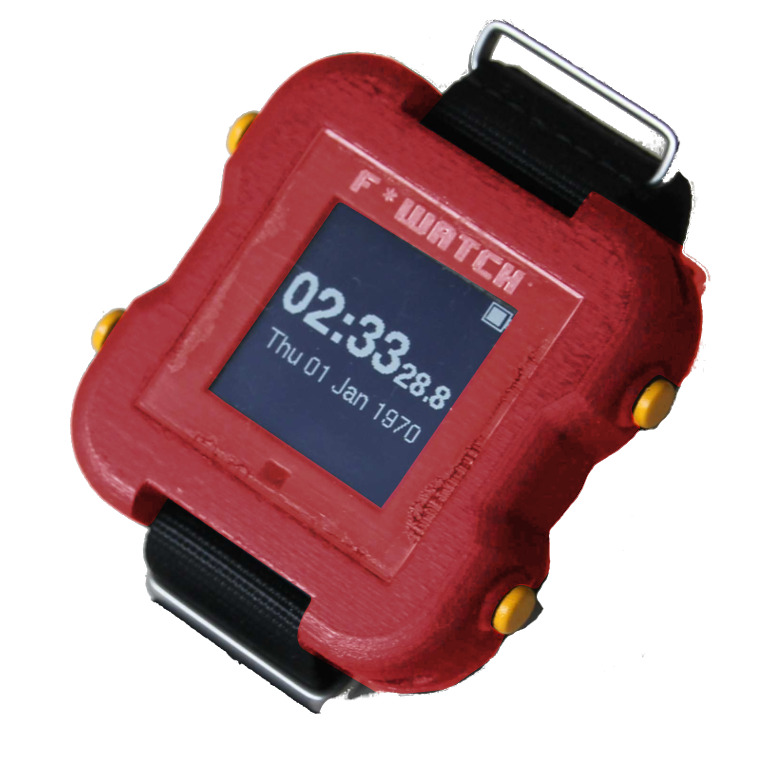
\includegraphics[height=7.5cm]{fwatch-full-side-red.eps}
      }{
        
\includegraphics[height=7.5cm]{fwatch-full-side-black-qmark.eps}
      }
  \end{center}
  \note[item]{This is a GPS watch}
  \note[item]{A lot of sensors}
  \note[item]{B/W screen}
  \note[item]{no touch screen --- buttons}
  \note[item]{other components --- not all}
  \note[item]{GPS module}
  \note[item]{it can run applications (smart watch)}
  \note[item]{Free product}
\end{frame}

%------------ FRAME --------------------------------------------------
\begin{frame}{Why a watch?}
  \Large
  \begin{center}
    Retirement gift for a timing Hacker \\
  \end{center}
  \vskip 1cm

  \textbf{Gift Requirement}
  \vskip 7mm
  \begin{enumerate}
  \item customization of the gift
    %\vskip mm
  \item hackable gift
    %\vskip 7mm
  \item free/open source
    %\vskip 7mm
  \item use only FOSS tools
  \end{enumerate}

  \note[item]{Retirement timing hacker}
  \note[item]{currently, not free smart device}
  \note[item]{challenge do it --- with free tools}

\end{frame}

%------------ FRAME --------------------------------------------------
\begin{frame}{Development organization}
  \begin{center}
    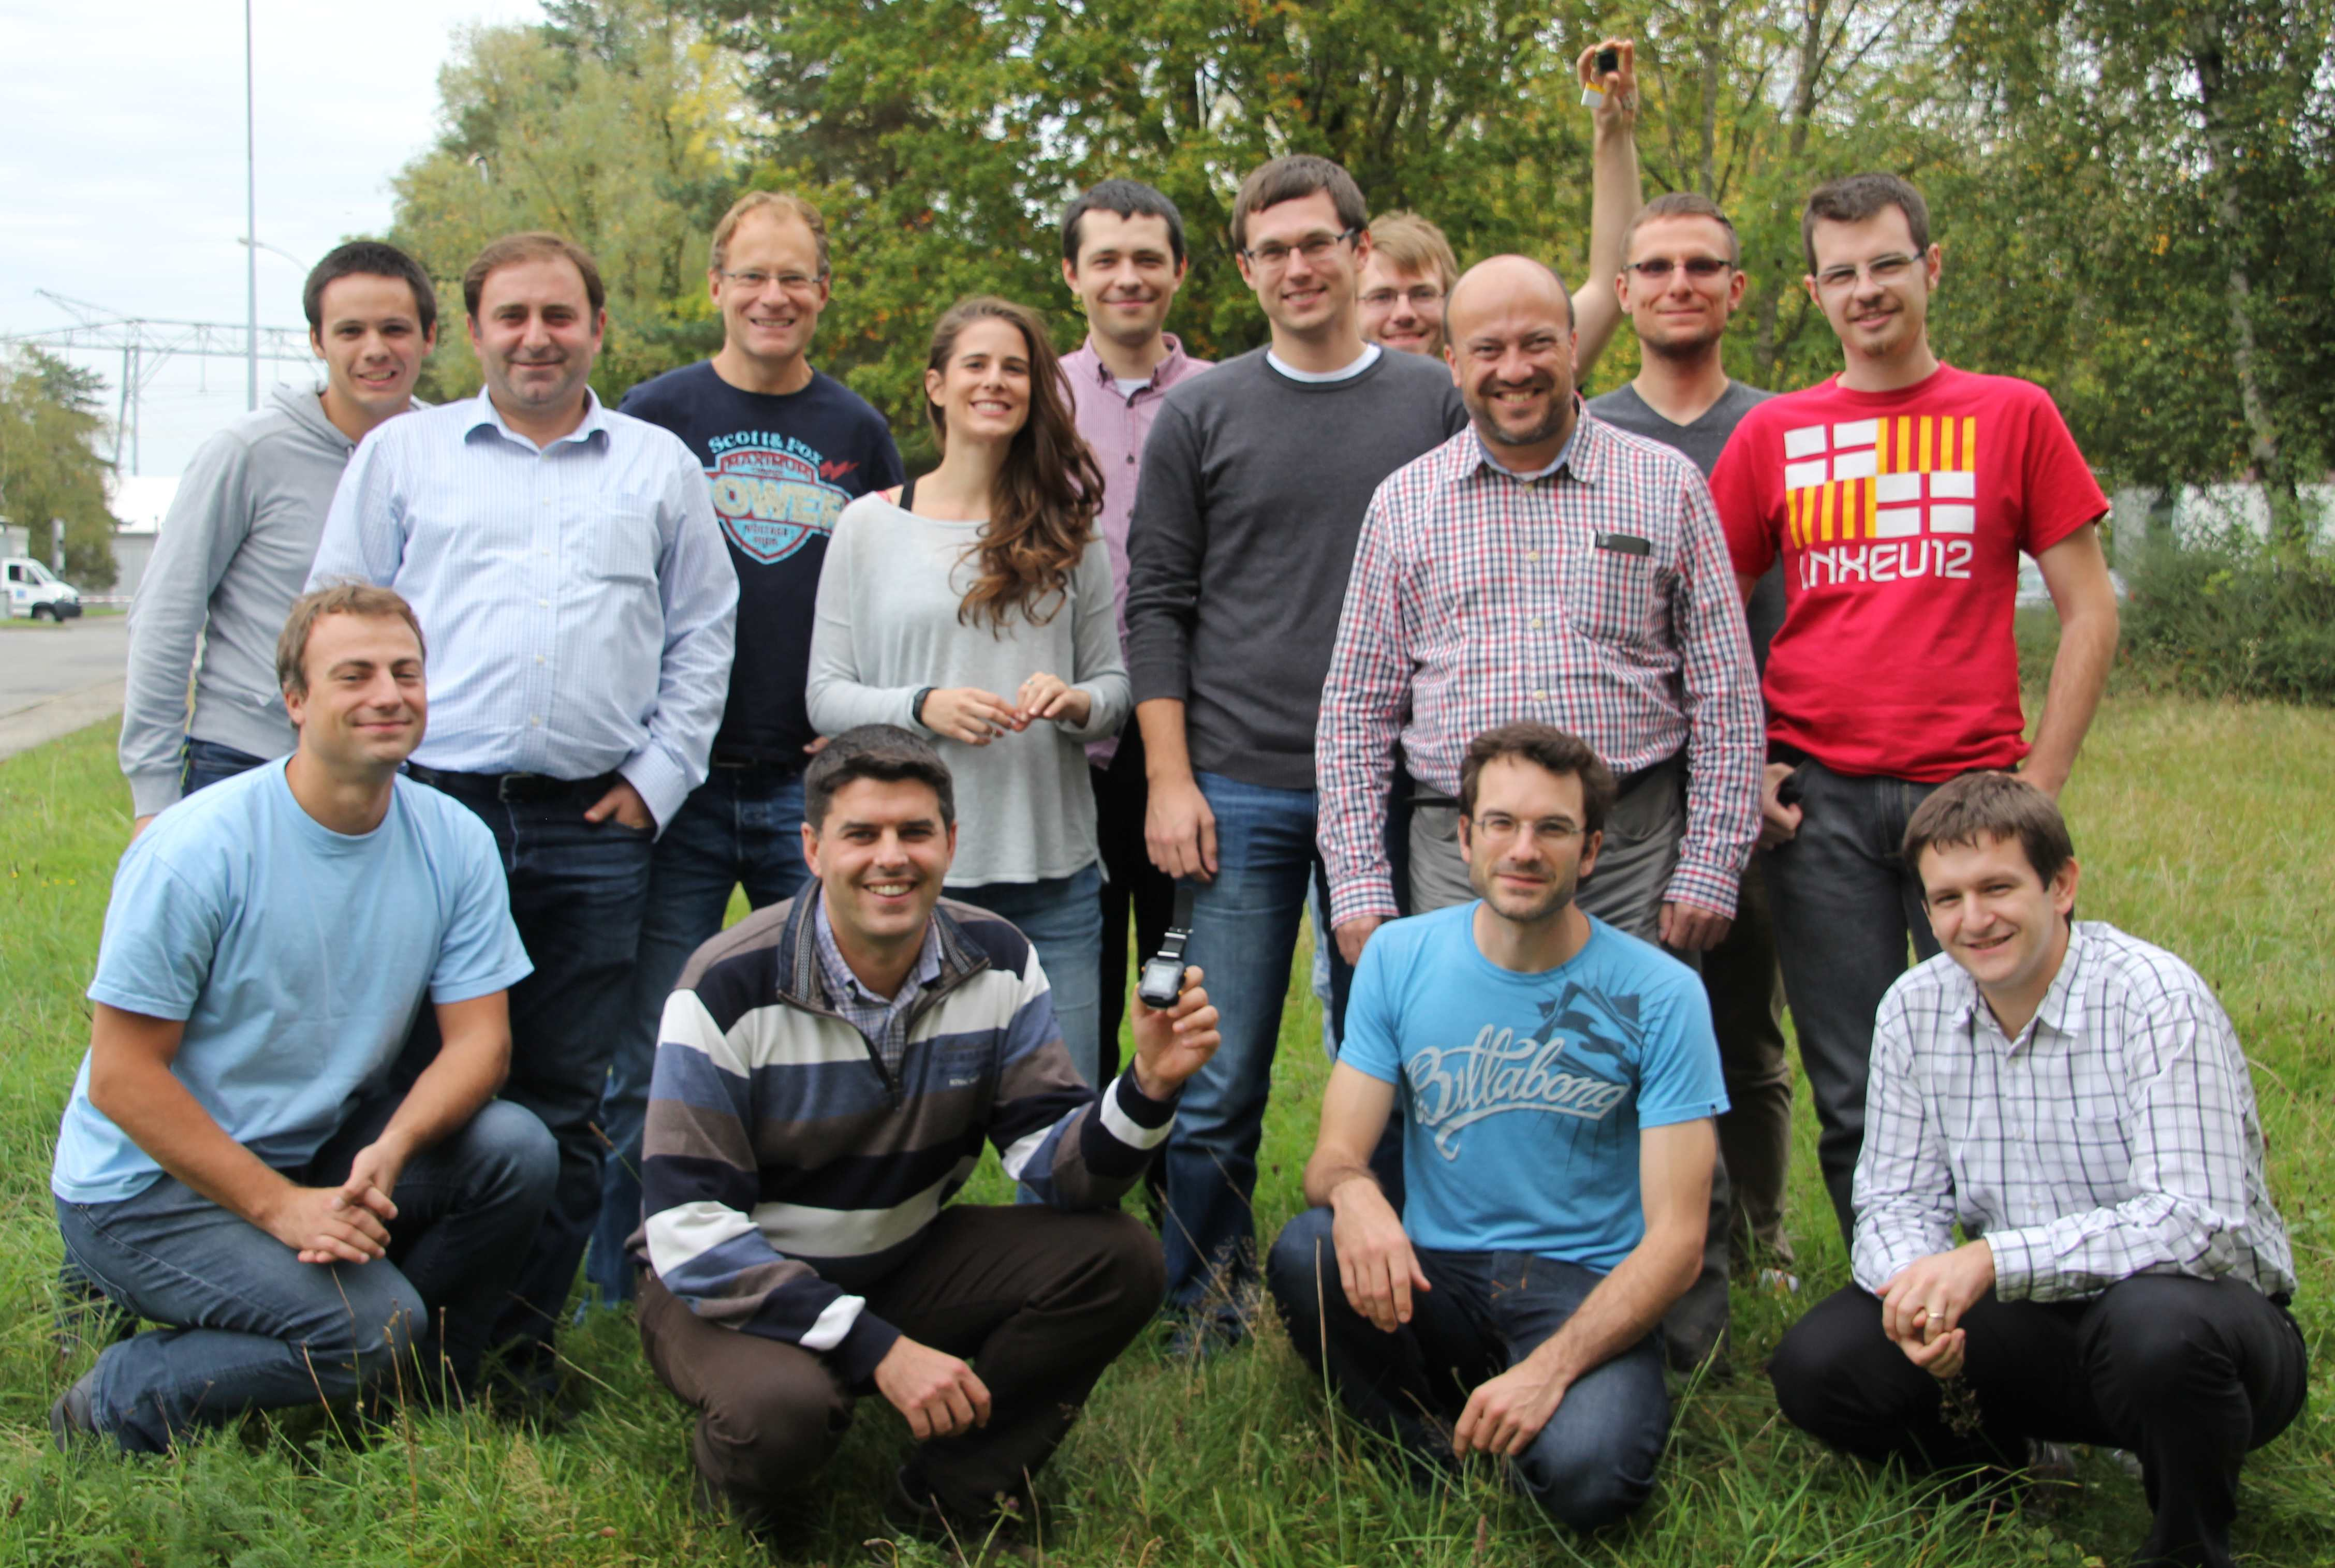
\includegraphics[height=7cm]{fwatch-team.eps}
  \end{center}

  \note[item]{people more or less involved}
  \note[item]{less than 5 months}
  \note[item]{after-work --- only free time}
  \note[item]{3 groups : mechanic, electronic, software}
  \note[item]{weekly meeting}
  \note[item]{introduce Matthieu}
\end{frame}

%------------ FRAME --------------------------------------------------
%% \Large
%% \begin{frame}{Features}
%%   \begin{itemize}
%%     \item Low power MCU
%%     \item LCD display
%%     \item Sensors
%%     \item I/O interface
%%     \item GPS module
%%   \end{itemize}
%% \end{frame}


%#####################################################################
%############ SECTION ################################################
\section{The design}

%------------ FRAME --------------------------------------------------
\begin{frame}{The design}

  Components selection criteria
  \vskip 5mm

  \begin{itemize}
  \item Low power consumption
    \vskip 5mm
  \item Available in small quantity from main suppliers
    \vskip 5mm
  \item Small size (footprint)
  \end{itemize}

  %\note[item]{Fill up slide??}
  %\note[item]{Talk about feasibility study??}
  \note[item]{After this introduction, I'll talk more about design process}
  \note[item]{We started with the component selection}
  \note[item]{All components must be low power, to have the longest possible battery life}
  \note[item]{They should be available from main suppliers in small quantity}
  \note[item]{$\rightarrow$ to allow others to build the watch}
  \note[item]{Also the components must be as small as possible to fit in a watch}

\end{frame}

%------------ FRAME --------------------------------------------------
\begin{frame}{Components selection}

  \begin{columns}[T] % align columns
    \begin{column}{.48\textwidth}

      Micro-controller
      \vskip 6mm
      \begin{itemize}
      \item Silicon Labs
      \item 13 x 9.5 x 1.8mm
      \item 32-bit Cortex-M3
      \item 1MB flash
      \item 128kB RAM
      \item 1.1uA deep sleep
      \end{itemize}

    \end{column}
    \hfill%
    \begin{column}{.48\textwidth}
      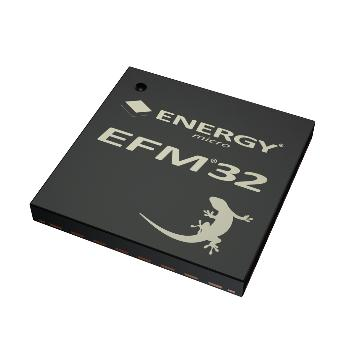
\includegraphics[height=5cm]{mcu_efm32.eps}
    \end{column}%
  \end{columns}

  %\note[item]{More detail about the MCU selection??}
  \note[item]{The micro controller we chose is a 32-bit cortex-M3 from Silicon Labs}
  \note[item]{It has a lot of memory}
  \note[item]{And an extremely low power consumption}
  \note[item]{In deep sleep mode it only consumes a few micro amperes}
  \note[item]{In deep sleep, the RTC is running and RAM is kept}


\end{frame}

%------------ FRAME --------------------------------------------------
\begin{frame}{Components selection}

  \begin{columns}[T] % align columns
    \begin{column}{.48\textwidth}

      GPS module
      \vskip 6mm
      \begin{itemize}
      \item Antenova
      \item 13 x 9.5 x 1.8mm
      \item Integrated antenna
      \end{itemize}

    \end{column}
    \hfill%
    \begin{column}{.48\textwidth}
      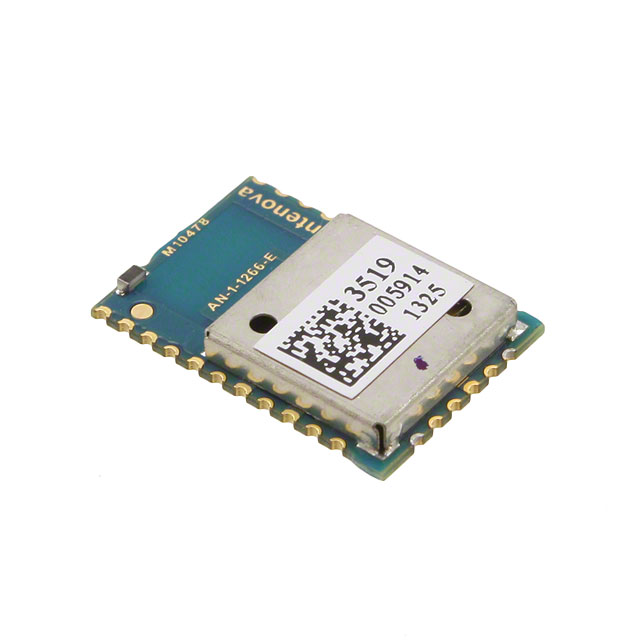
\includegraphics[height=5cm]{M10478-A1.eps}
    \end{column}%
  \end{columns}

  \note[item]{The main component of a GPS watch is of course the GPS module}
  \note[item]{We chose a module with integrated antenna from Antenova, to simplify the design and reduce the risk}
  \note[item]{Because designing a specific on-board antenna can be tricky}
  \note[item]{And we are not RF experts}

\end{frame}

%------------ FRAME --------------------------------------------------
\begin{frame}{Components selection}

  \begin{columns}[T] % align columns
    \begin{column}{.48\textwidth}

      Altimeter module \\
      (pressure sensor)
      \vskip 6mm
      \begin{itemize}
      \item Measurement Specialties
      \item 6.4 x 4 x 2.8mm
      \item Water-resistant
      \item Includes a thermometer
      \end{itemize}

    \end{column}
    \hfill%
    \begin{column}{.48\textwidth}
      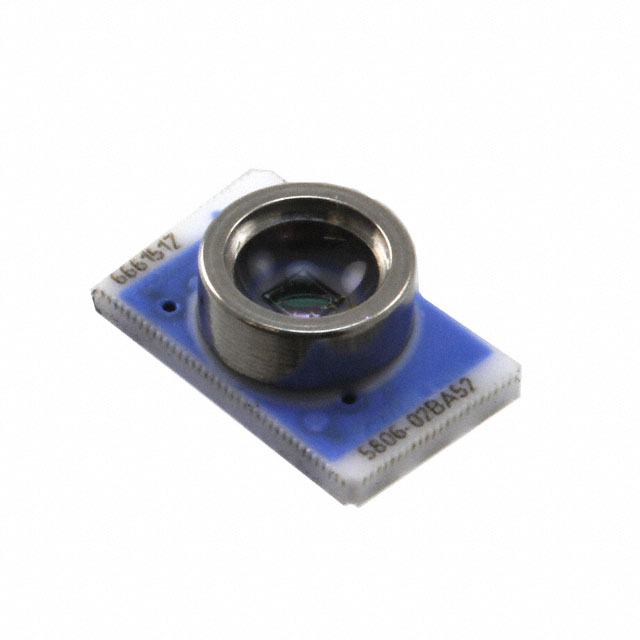
\includegraphics[height=4.5cm]{MS5806-02BA52-51.eps}
    \end{column}%
  \end{columns}

  \note[item]{Another important component is the pressure sensor}
  \note[item]{Because we wanted this watch to be a hiking and mountaineering watch}
  \note[item]{So we needed a good pressure sensor to calculate the altitude precisely}
  \note[item]{Because the GPS is quite inaccurate for the altitude}
  \note[item]{And also the pressure sensor can be used to give a basic weather forecast}
  \note[item]{We chose a very good pressure sensor}
  \note[item]{It is water-resistant, it's important because it has to be exposed to the outside of the case}
  \note[item]{And it includes a thermometer}
  \note[item]{Of course, the temperature is not very accurate when you have the watch on you wrist}

\end{frame}

%------------ FRAME --------------------------------------------------
\begin{frame}{Components selection}

  \begin{columns}[T] % align columns
    \begin{column}{.48\textwidth}

      Memory LCD display
      \vskip 6mm
      \begin{itemize}
      \item Sharp
      \item 128 x 128 pixels
      \item 1.28 inches
      \item Ultra low current
      \end{itemize}

    \end{column}
    \hfill%
    \begin{column}{.48\textwidth}
      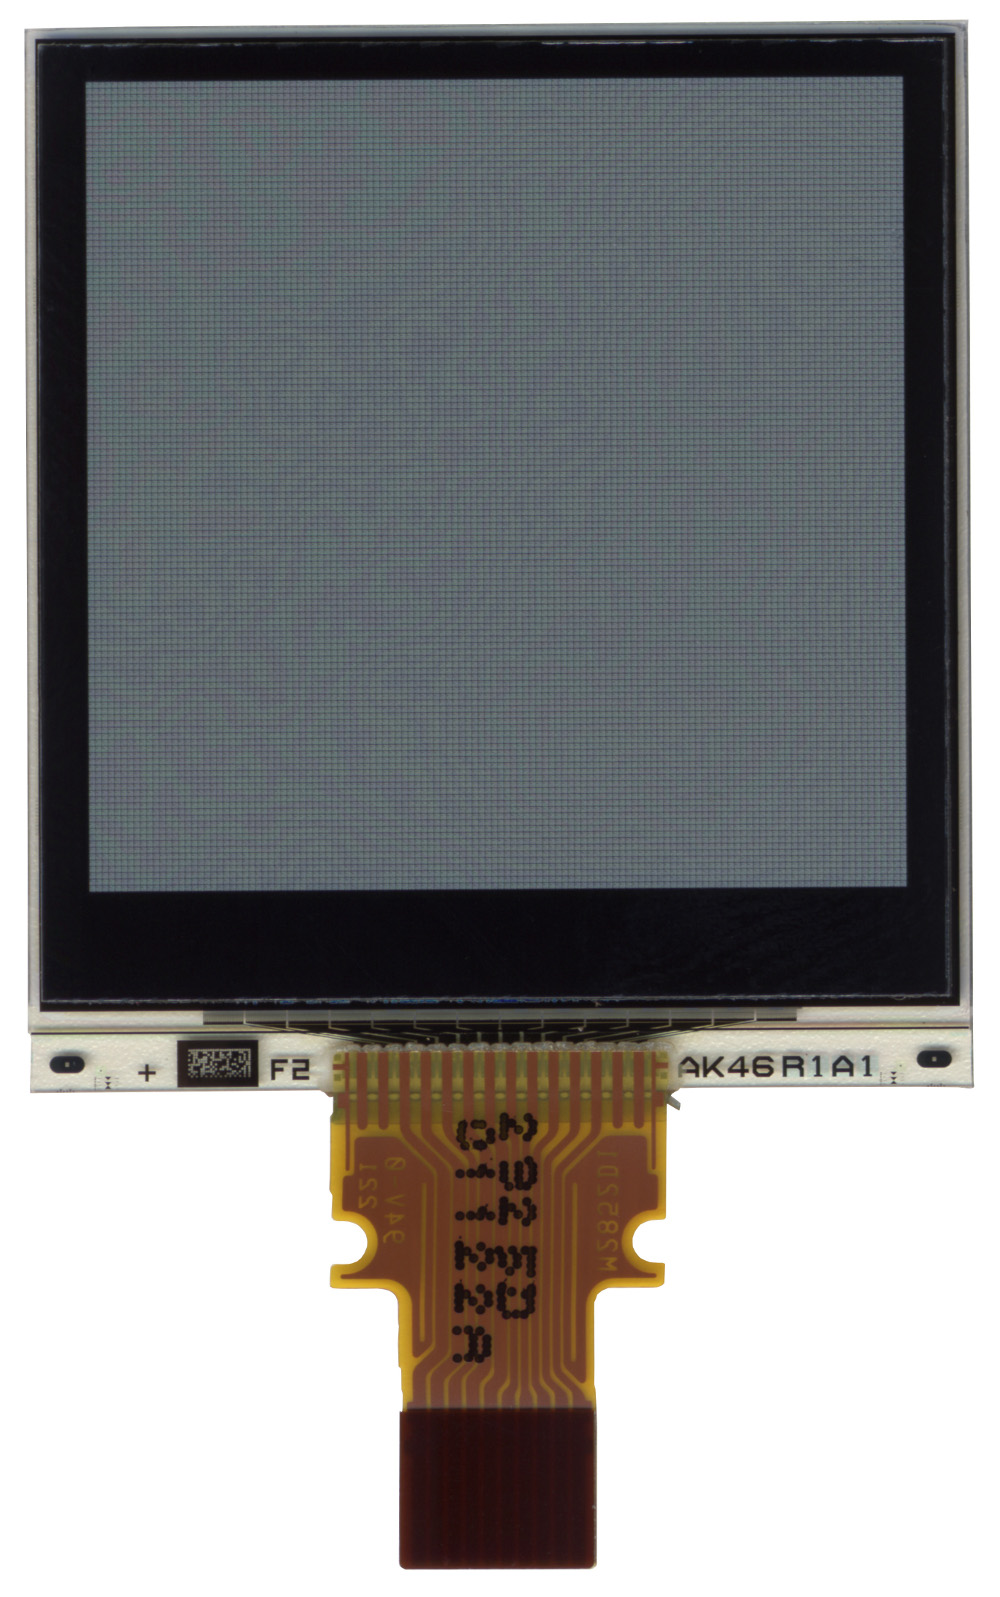
\includegraphics[height=4.5cm]{LCD.eps}
      %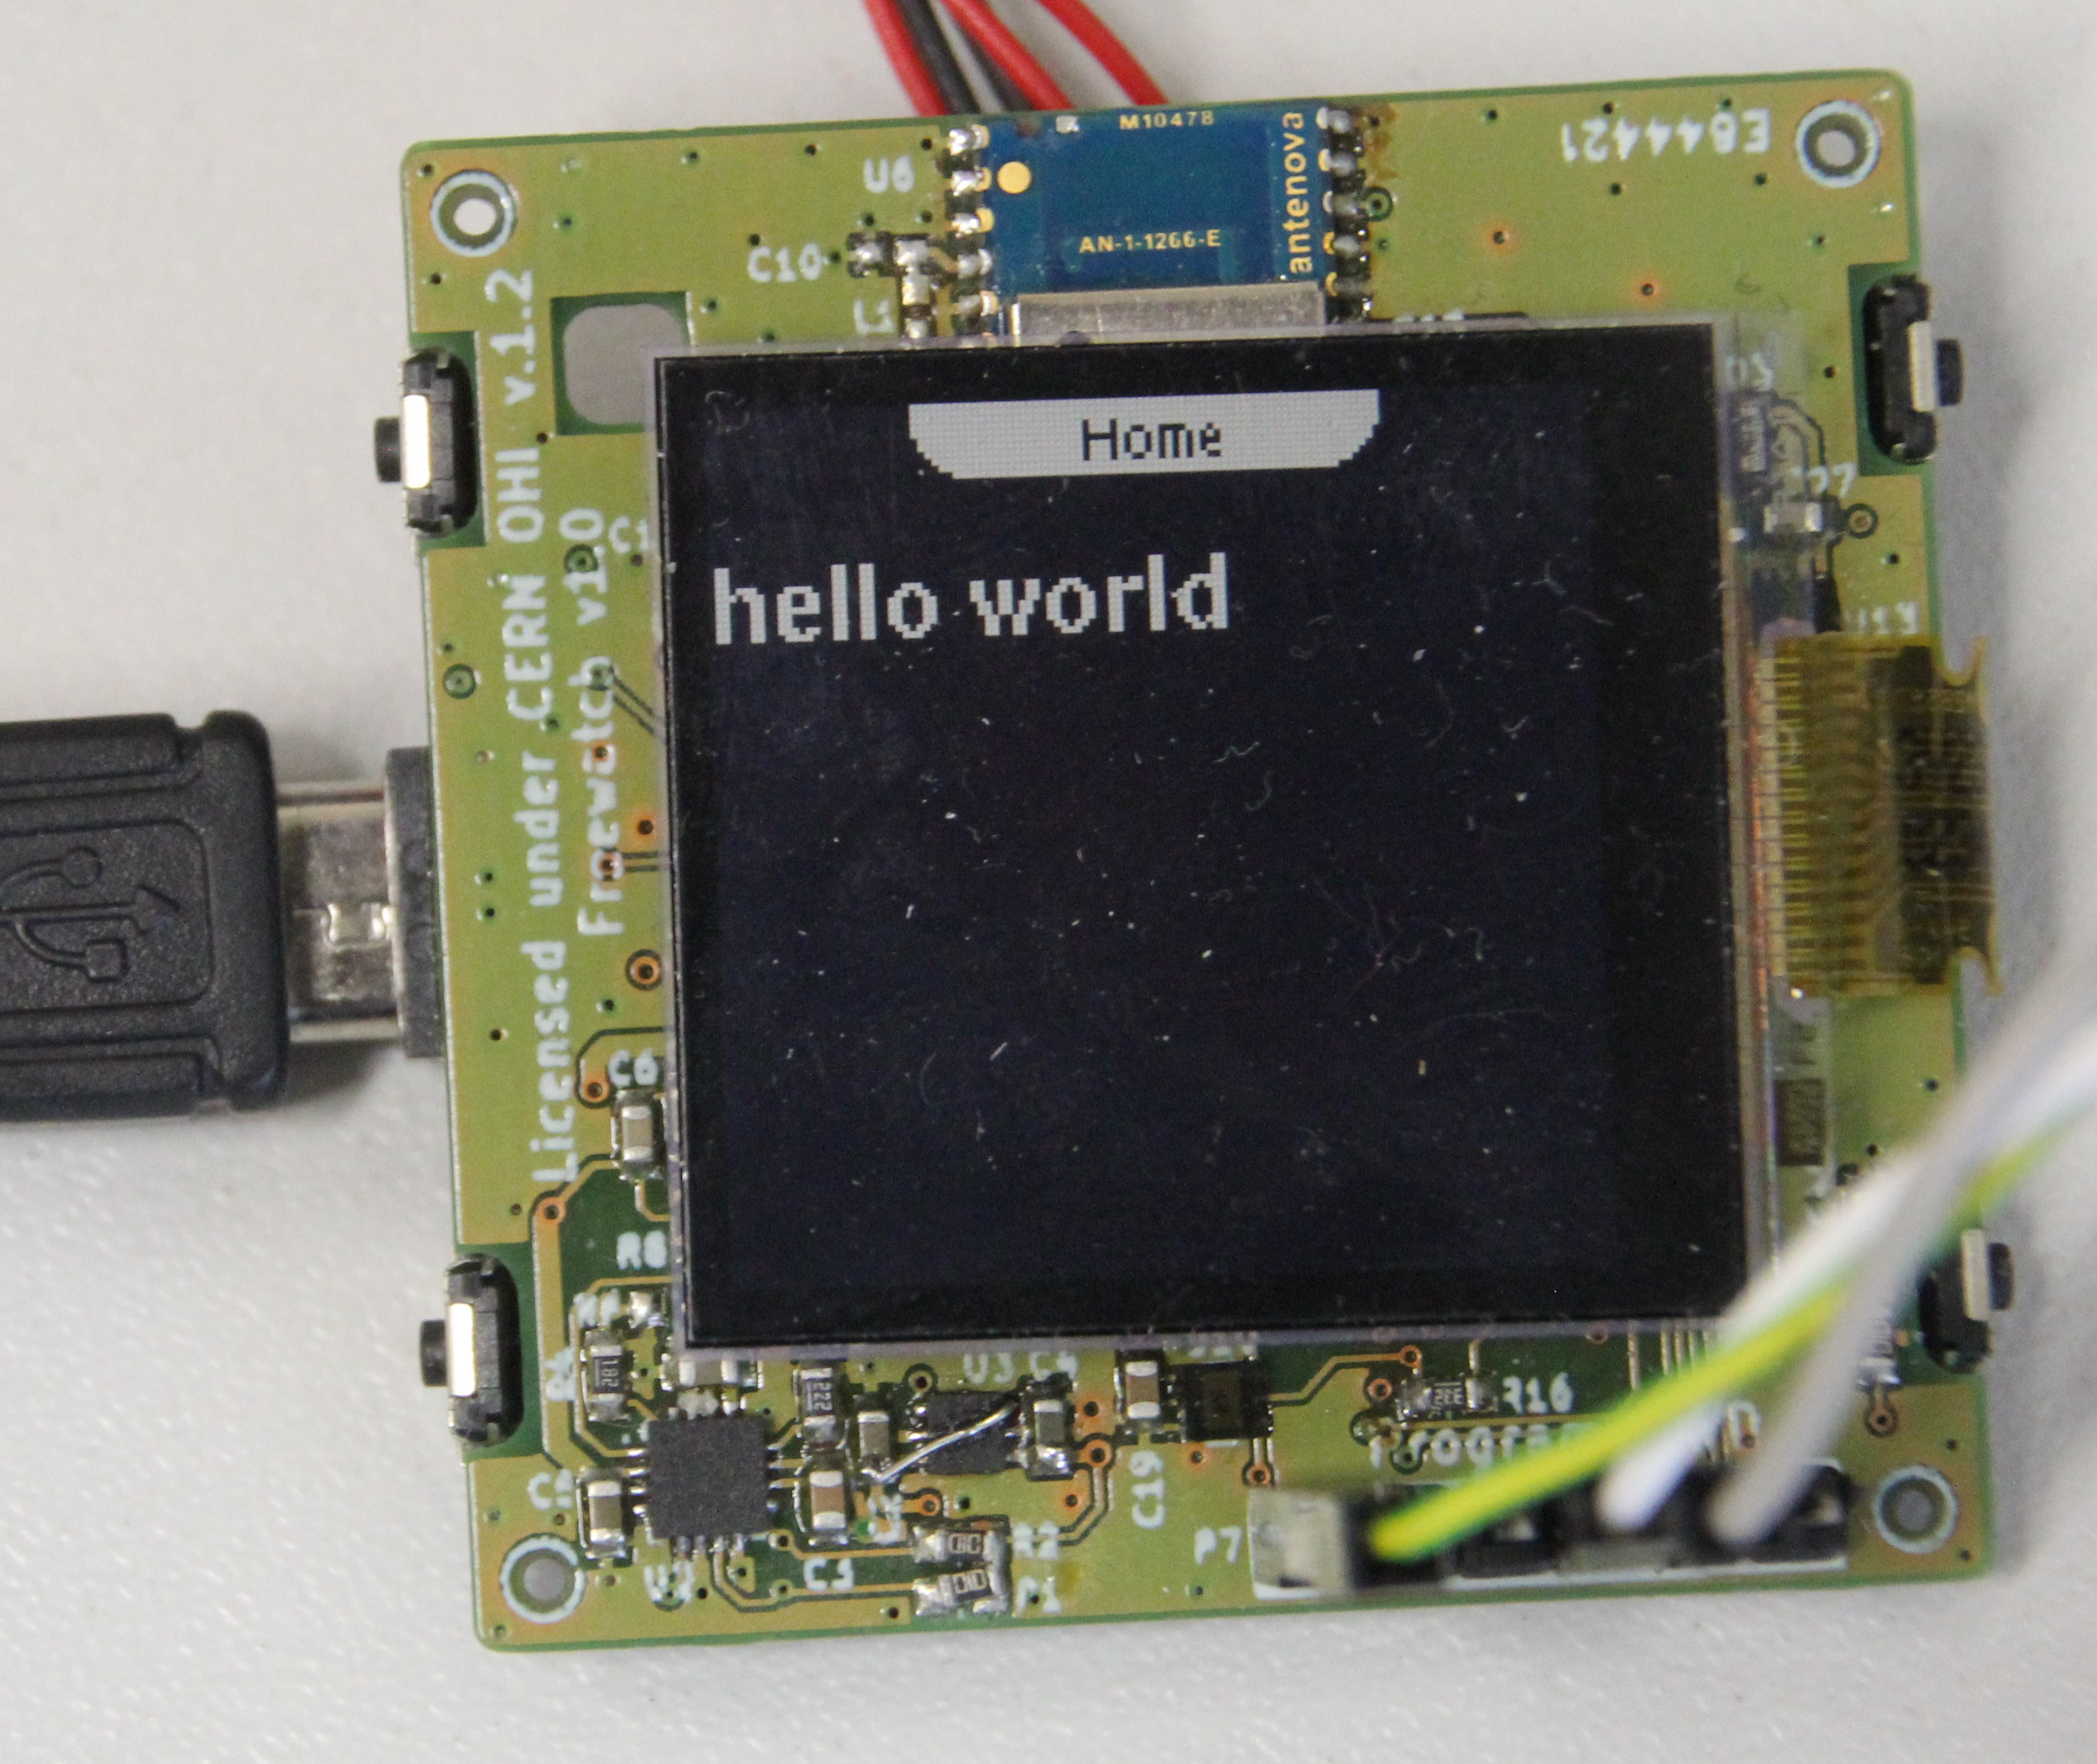
\includegraphics[height=4.5cm]{sw_hello_world.eps}
    \end{column}%
  \end{columns}

  %\note[item]{Replace by hello world picture??}
  \note[item]{For the display, we chose a memory LCD from Sharp}
  \note[item]{It's 128 by 128 pixel, for 1.28 inches (~3cm)}
  \note[item]{This LCD requires a very low current to keep the image, because it has a memory in each pixel}
  \note[item]{It is readable in sunlight}
  \note[item]{A backlight is useful only to read it in the dark, we'll come to this later}

\end{frame}

%------------ FRAME --------------------------------------------------
\begin{frame}{Components selection}

  \begin{columns}[T] % align columns
    \begin{column}{.48\textwidth}

      Battery
      \vskip 6mm
      \begin{itemize}
      \item Adafruit
      \item Li-ion 500mAh
      \item Big capacity
      \item Lightweight
      \item Rechargeable
      \end{itemize}

    \end{column}
    \hfill%
    \begin{column}{.48\textwidth}
      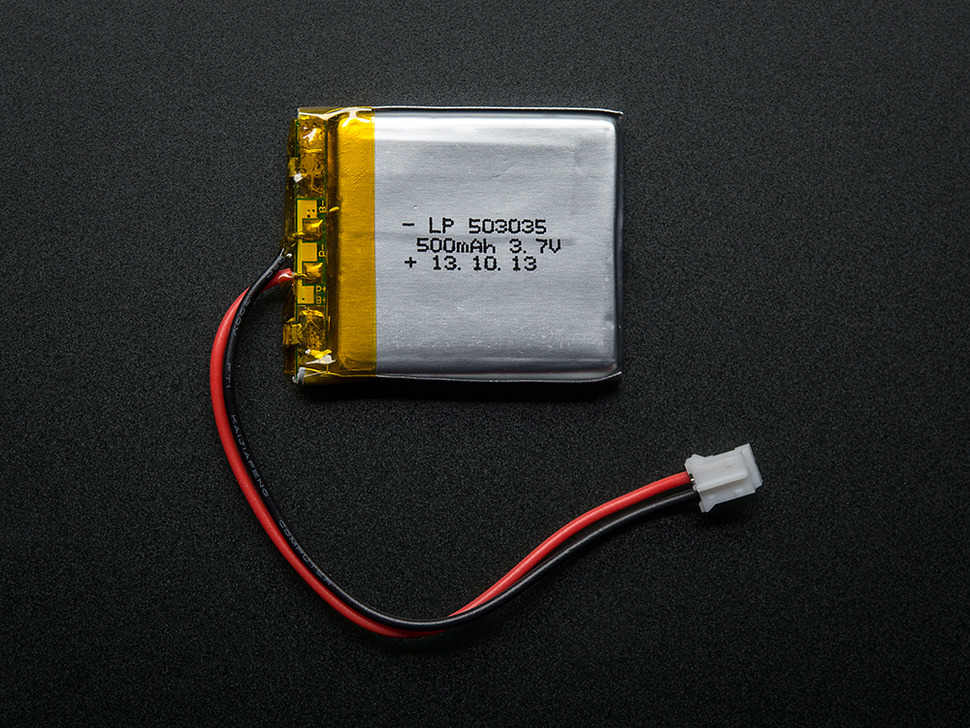
\includegraphics[height=4.5cm]{battery.eps}
    \end{column}%
  \end{columns}

  \note[item]{The battery we chose is a 500mAh Lithium ion bought via Adafruit}
  \note[item]{It has a big capacity, because the GPS module consumes quite a lot}
  \note[item]{It is very light}
  \note[item]{And it is of course rechargeable}

\end{frame}

%------------ FRAME --------------------------------------------------
\begin{frame}{Components selection}

  Other features
  \begin{itemize}
  \item 3-axis accelerometer + compass
  \item Ambient light sensor
  \item micro-SD card slot
  \item Battery charger + fuel gauge
  \item micro-USB connector
  \item Buzzer
  \item Vibrating motor
  \end{itemize}

  \vskip 5mm
  Foreseen improvements
  \begin{itemize}
  \item Bluetooth LE
  \item Low noise amplifier for the GPS antenna
  \item Power management
  \end{itemize}

  \begin{center}
    %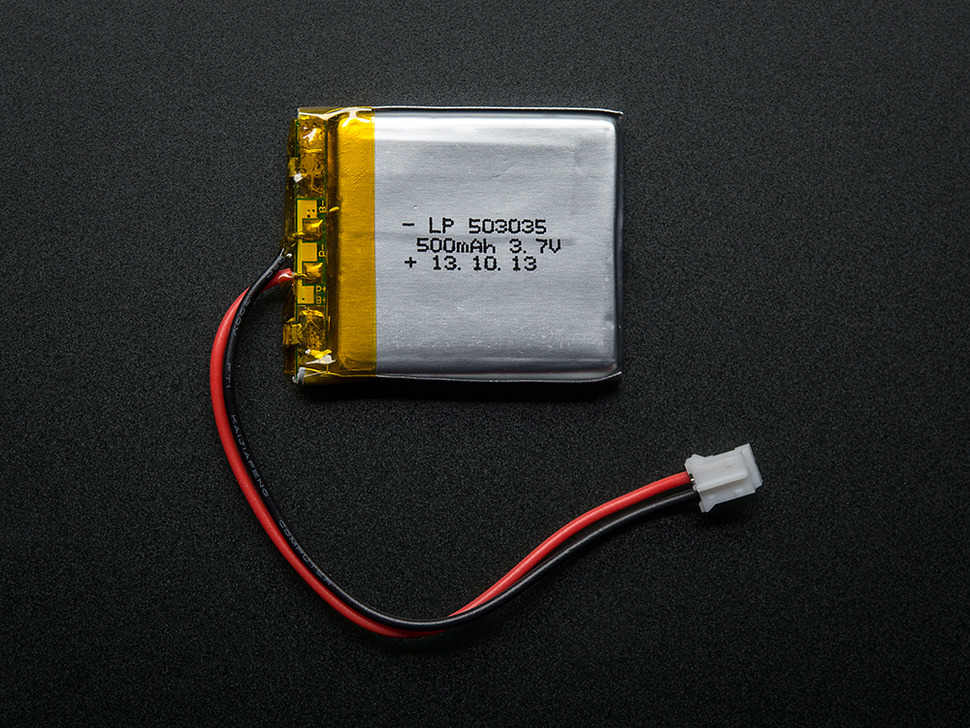
\includegraphics[height=5cm]{battery.eps}
  \end{center}

  \note[item]{micro-SD card to store for example GPS tracks}
  \note[item]{USB is used for battery charging, firmware upload, data transfer}
  \note[item]{It also includes a buzzer and a vibrating motor to notify the user}
  \note[item]{Bluetooth for wireless sensors $\rightarrow$ heart-rate monitor, ...}
  \note[item]{Low noise amplifier to improve GPS sensitivity}
  \note[item]{Improve power management $\rightarrow$ save battery}

\end{frame}

%------------ FRAME --------------------------------------------------
\begin{frame}{PCB design}

  %EDA tool choice

  \begin{center}
    
\includegraphics[height=1cm]{kicad_logo.eps}
  \end{center}

  \begin{itemize}
  \item CERN is contributing
  \item Developers in the team (help, bugfix, feedback)
  \item New features making routing easier (e.g push\&shove)
  \item Script to generate placement pdf
  \end{itemize}

  \vskip 6mm
  Interested in knowing more about KiCad developments?
  \begin{itemize}
  \item Visit the EDA dev room (AW1.124) tomorrow
  \end{itemize}

  %\note[item]{make advert. for contribution??}
  \note[item]{I will now talk about the PCB design}
  \note[item]{To design the pcb, we chose kicad}
  \note[item]{The choice was pretty straight forward, as cern is contributing to the project}
  %\note[item]{The reason cern is contributing is to improve open source design sharing}
  %\note[item]{The goal is to make it comparable to the mid-end commercial tools}
  \note[item]{Also we had kicad developers in the team}
  \note[item]{This was very useful to get quick help and bugfixes}
  \note[item]{On the other hand, the watch project allowed to systematically list all the points to be improved}
  \note[item]{When we started the pcb design, kicad just included the push\&shove function, it really made the routing easier}
  \note[item]{We also wrote a script to generate component placement pdf $\rightarrow$ for hand assembly}
  \note[item]{If you want to know more about kicad, it's feature and the future plans I invite you to visit the EDA dev room tomorrow}

\end{frame}

%------------ FRAME --------------------------------------------------
\begin{frame}{PCB design}

  Characteristics

  \begin{itemize}
  \item 4 x 4 cm
  \item 4 layers
  \item Components on both sides
  %\item Manufactured by Eurocircuits
  \item Licensed under CERN OHL v1.2
  \end{itemize}

  \begin{center}
    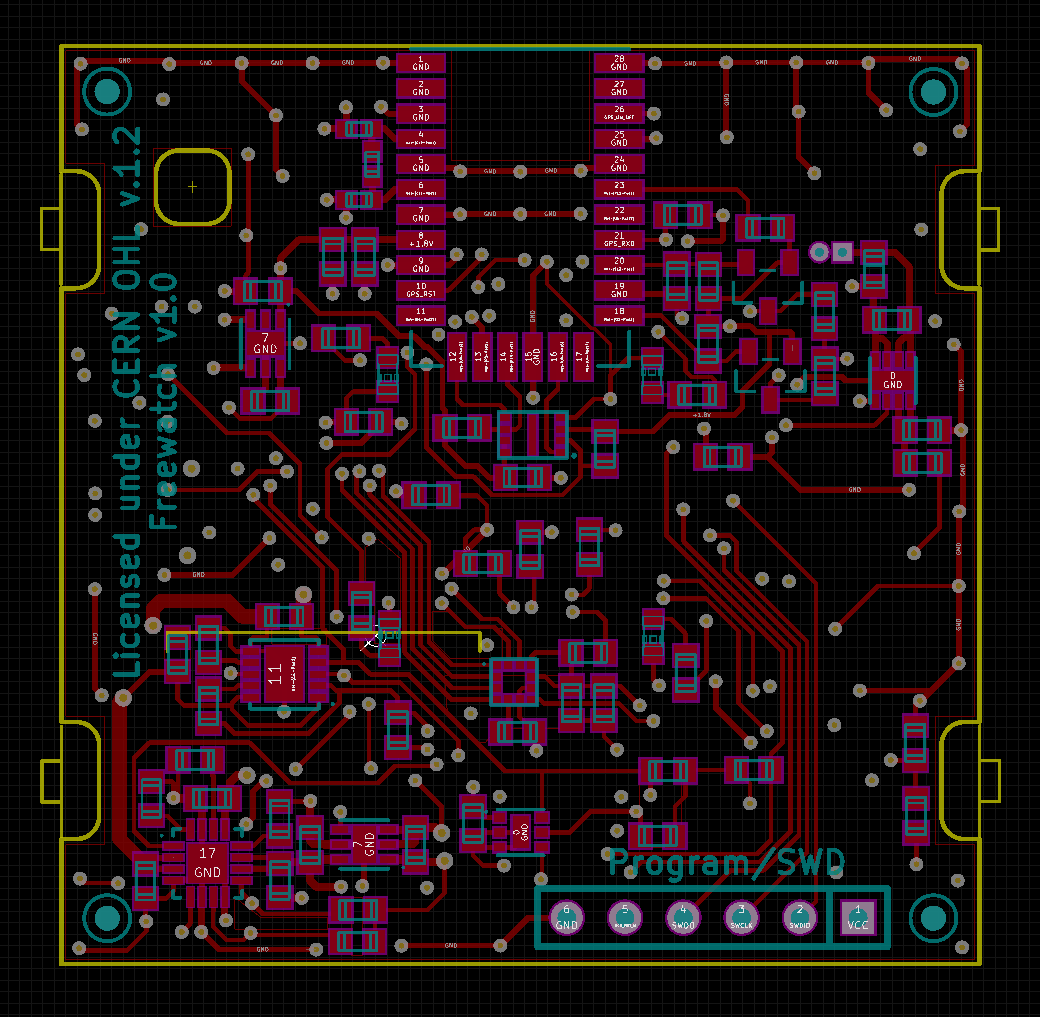
\includegraphics[height=4cm]{pcb_top.eps}~
    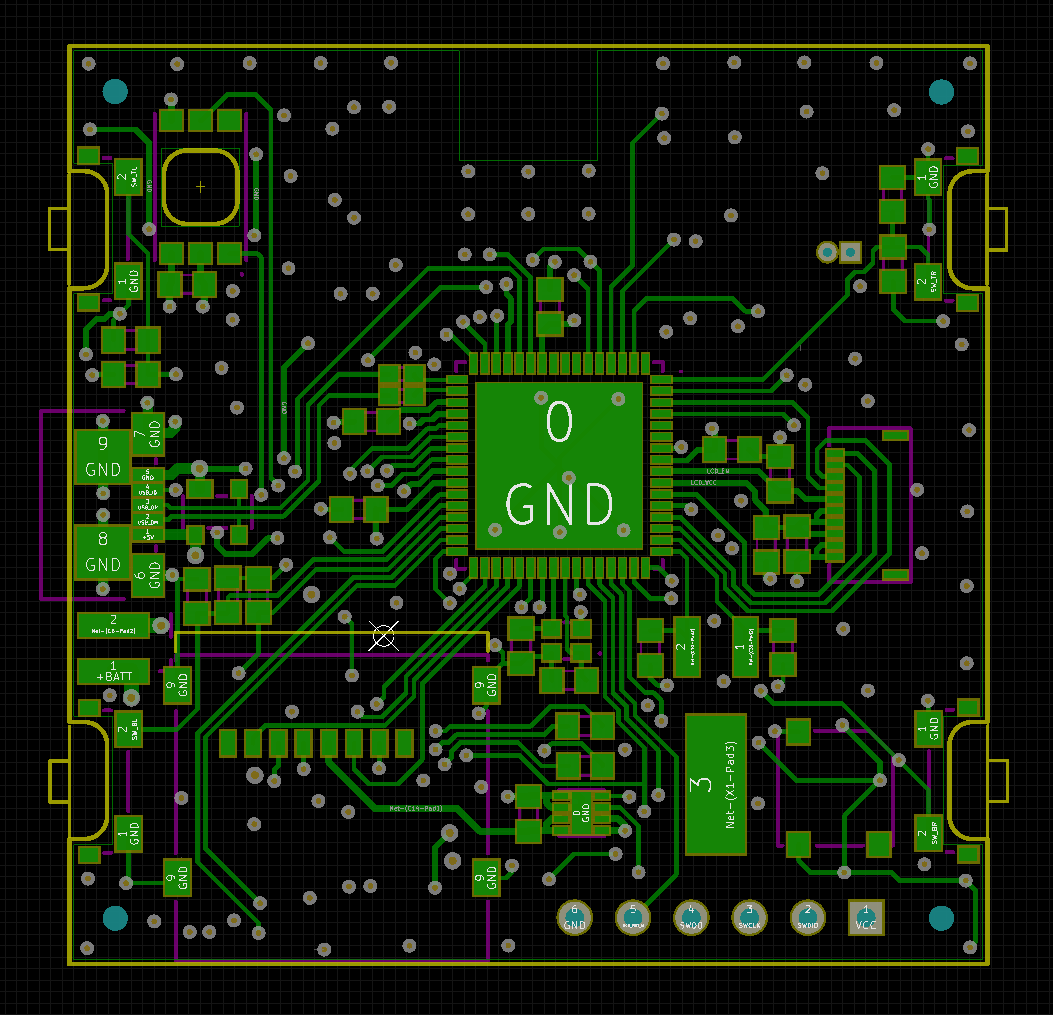
\includegraphics[height=4cm]{pcb_bottom.eps}
  \end{center}

  \note[item]{The goal was to fix every thing in a 4 by 4 cm board}
  \note[item]{There is two thing in opposition here}
  \note[item]{On one side the GPS reception is better with a big board}
  \note[item]{On the other side, it should fix in a watch}
  \note[item]{}
  \note[item]{there is still free space (without components)}
  \note[item]{Size could be reduced}
  \note[item]{Might need additional layers = extra cost}

\end{frame}

%------------ FRAME --------------------------------------------------
\begin{frame}{PCB assembly \& validation}

  Prototypes assembled by hand
  \vskip 5mm
  Fully working, except two minor bugs

  \begin{itemize}
  \item Error in a datasheet
    %\begin{itemize}
    %\item Voltage regulator output wrongly set
    %\end{itemize}
  \item MCU interrupt scheme
    %\begin{itemize}
    %\item Not all MCU pins as IRQ source
    %\item Polling drains the battery quickly
    %\end{itemize}
  \end{itemize}

  $\rightarrow$ Fixed with few cuts and wires!

  \begin{center}
    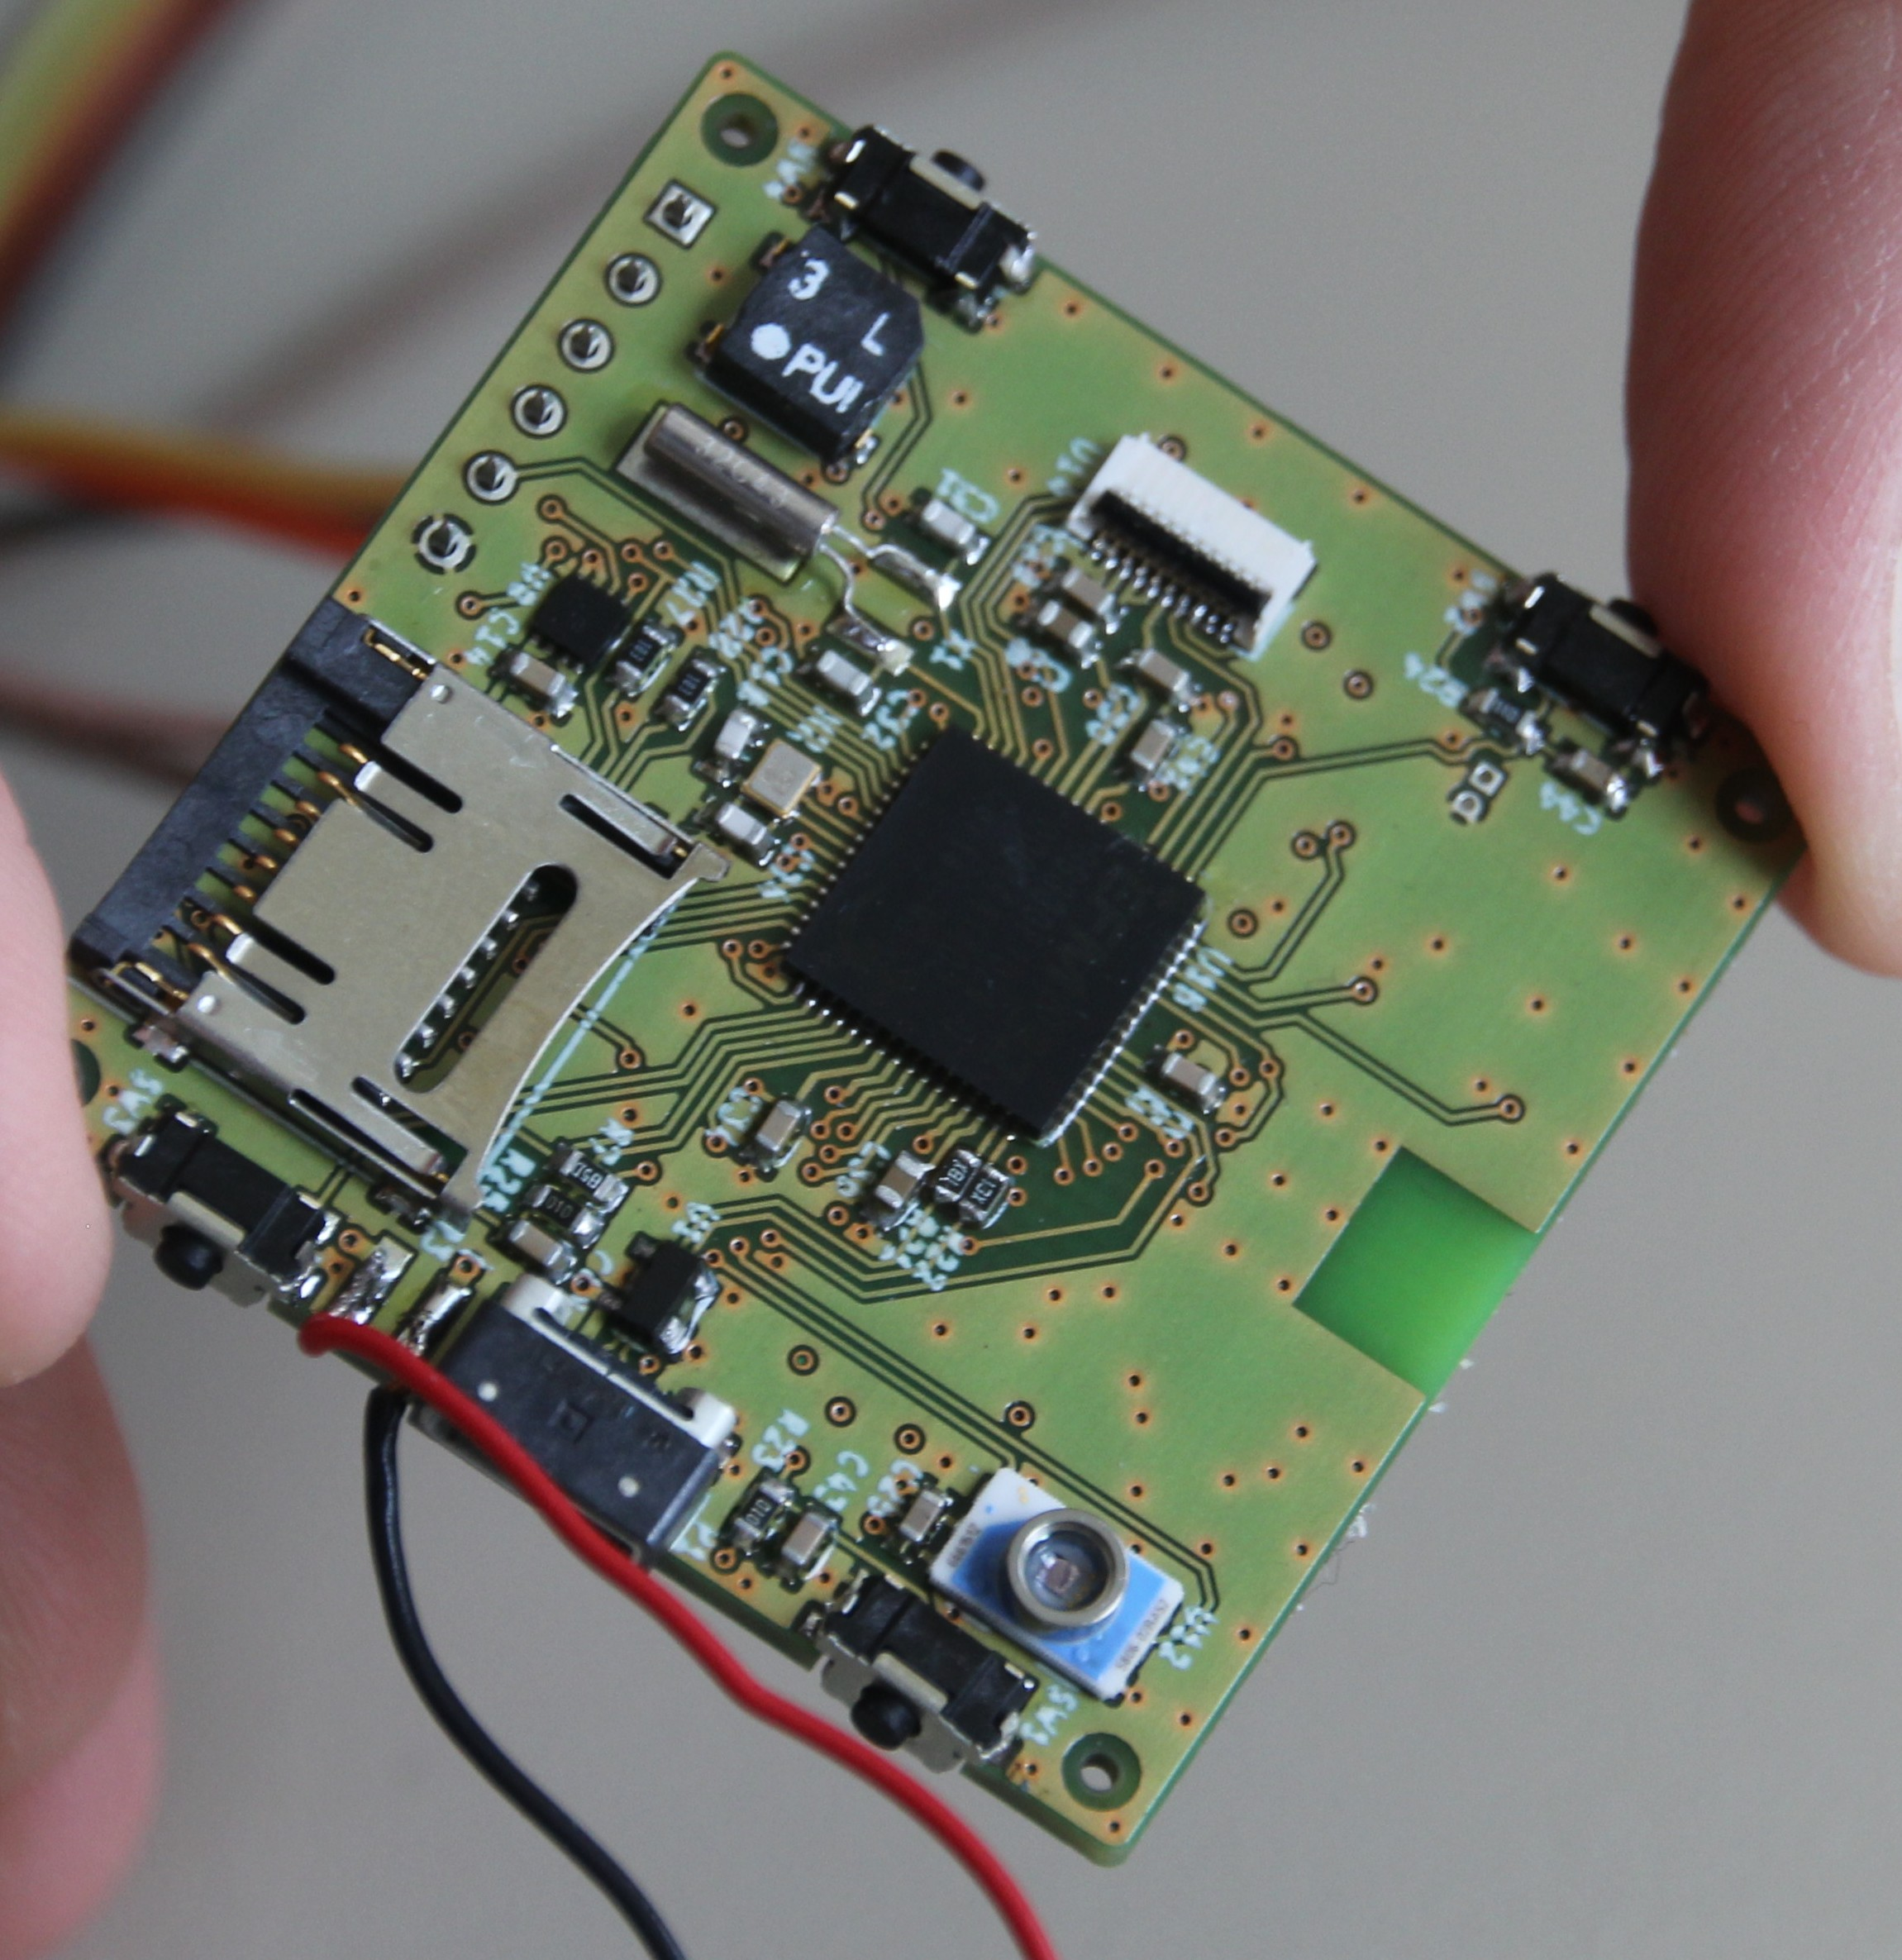
\includegraphics[height=3cm]{pcb_mounted_bottom.eps}~
    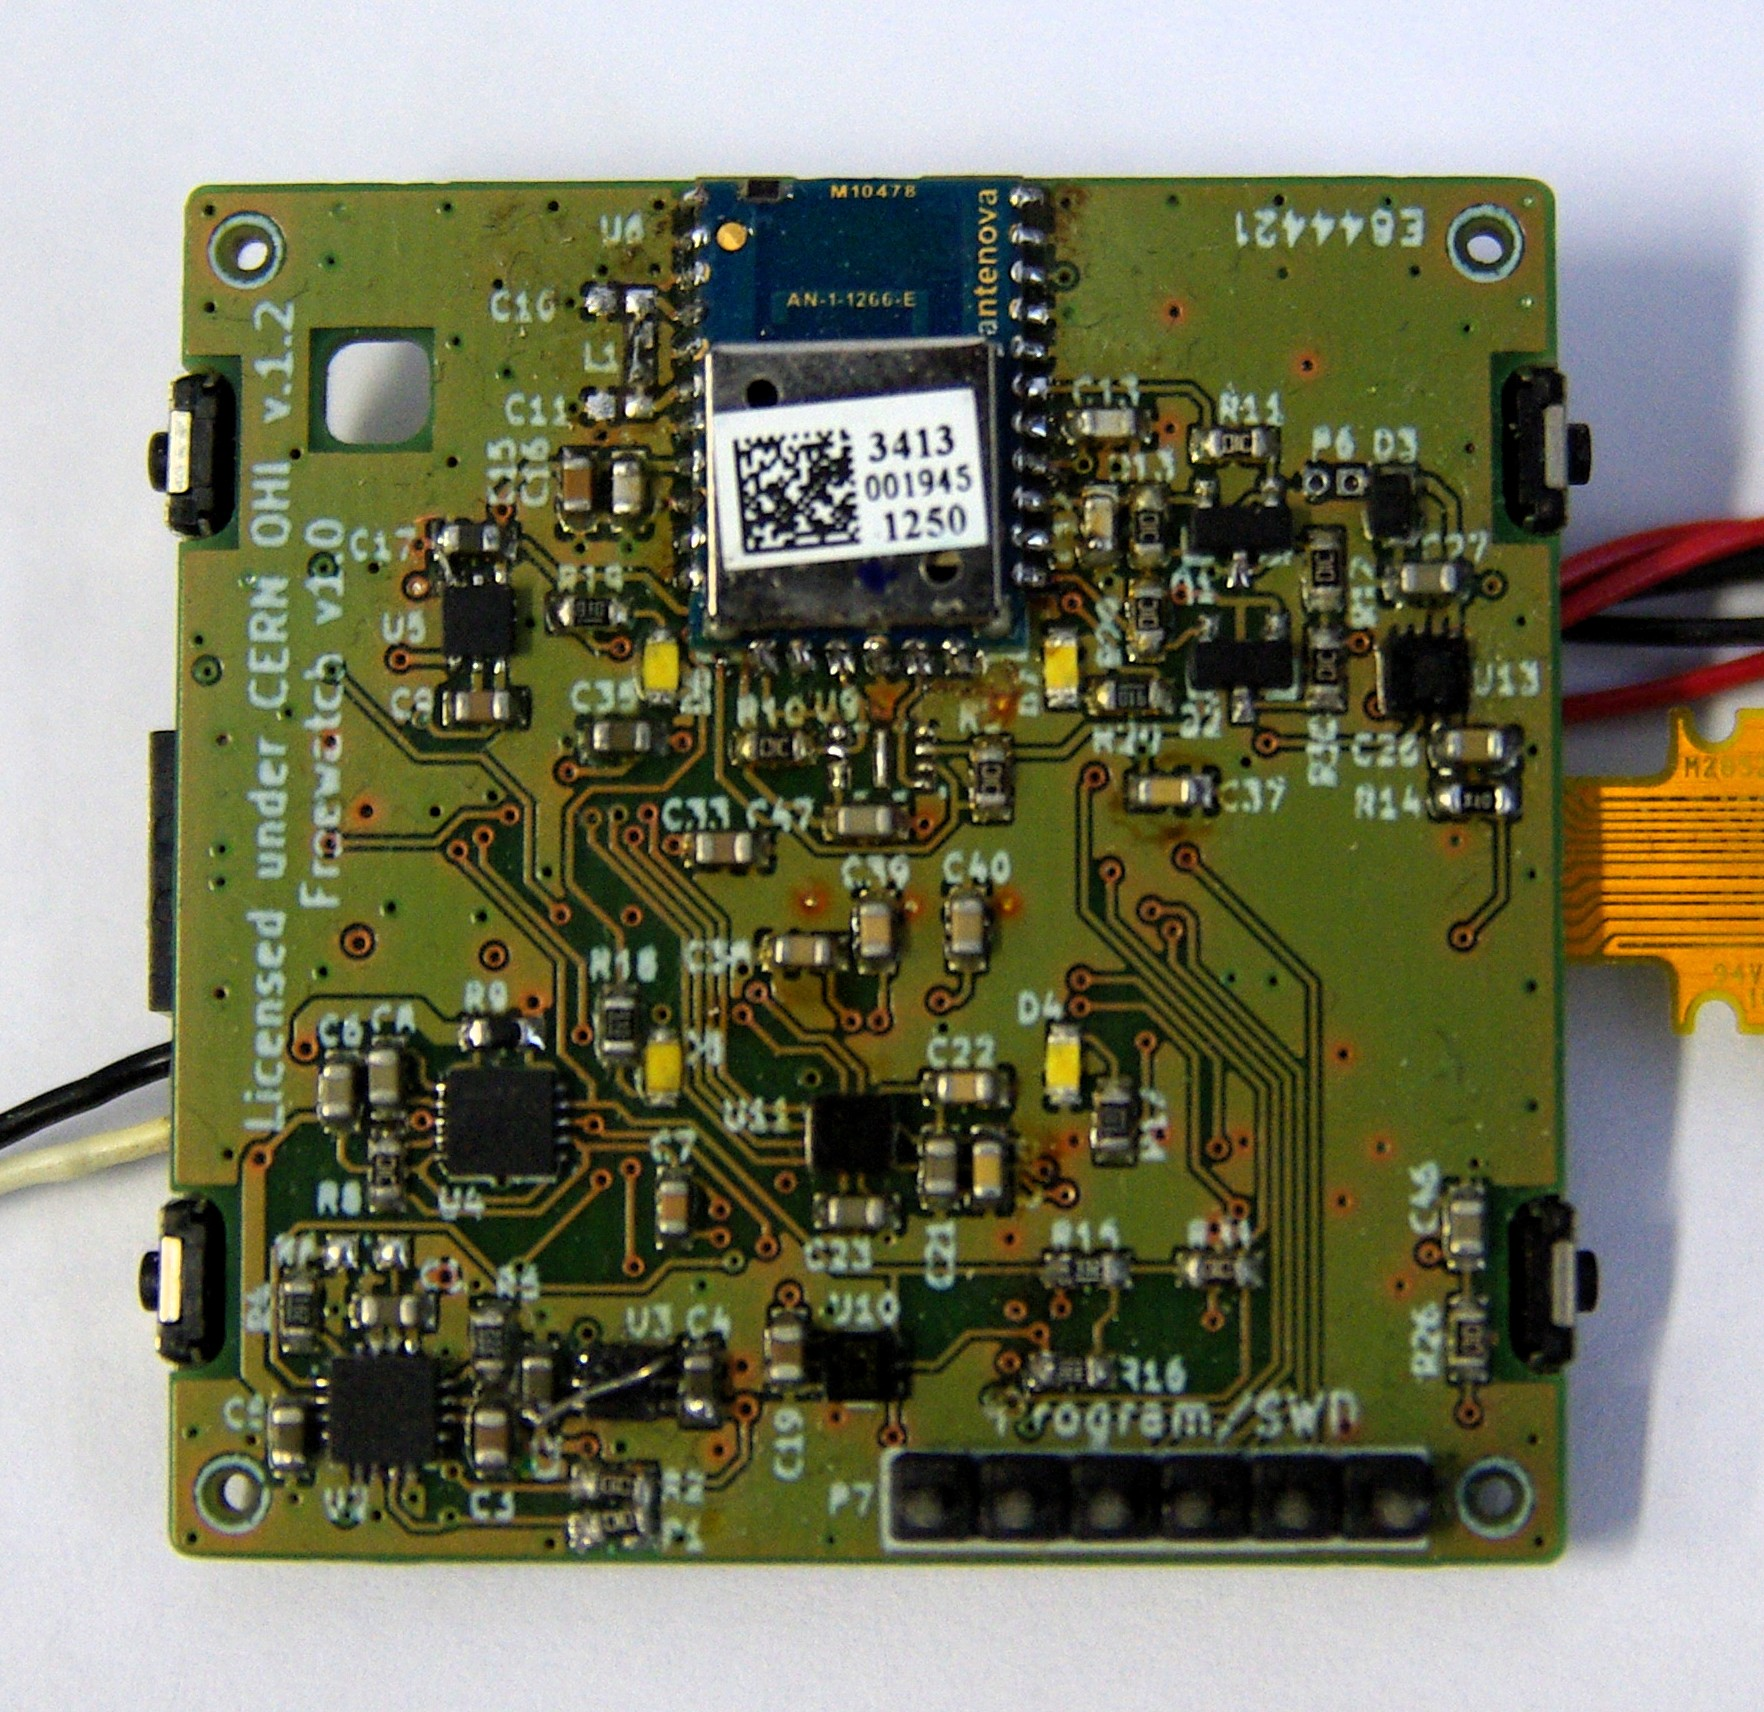
\includegraphics[height=3cm]{pcb_mounted_top.eps}
  \end{center}

  \note[item]{After routing the pcb, we order a few board that we assembled by hand}
  \note[item]{There were only one error that preveted the circuit to work properly}
  \note[item]{The voltage regulator setting pins was badly connected}
  \note[item]{This was due to a error in the datasheet it was easily fixed by cutting a trace and soldering a little wire}
  \note[item]{Also, we didn't carefully check how the interrupt work with this MCU and in order to use interrupt from the battery gauge and accelerometer, we had to solder a few exra wires}
  \note[item]{Because without interrupt we had to poll to check if the charger was plugged and it was draining the battery quickly.}

\end{frame}

%------------ FRAME --------------------------------------------------
\begin{frame}{Backlight}

  A long story...

  \note[item]{Another challenge was the backlight of the LCD display}
  \note[item]{As aI said, the LCD is perfectly readable during day, even under sunlight}
  \note[item]{But not in the dark or during the night}
  \note[item]{This is why we need a backlight}

\end{frame}

%------------ FRAME --------------------------------------------------
\begin{frame}{Backlight}

  First try: LEDs + opaque Plexiglas

  \begin{center}
    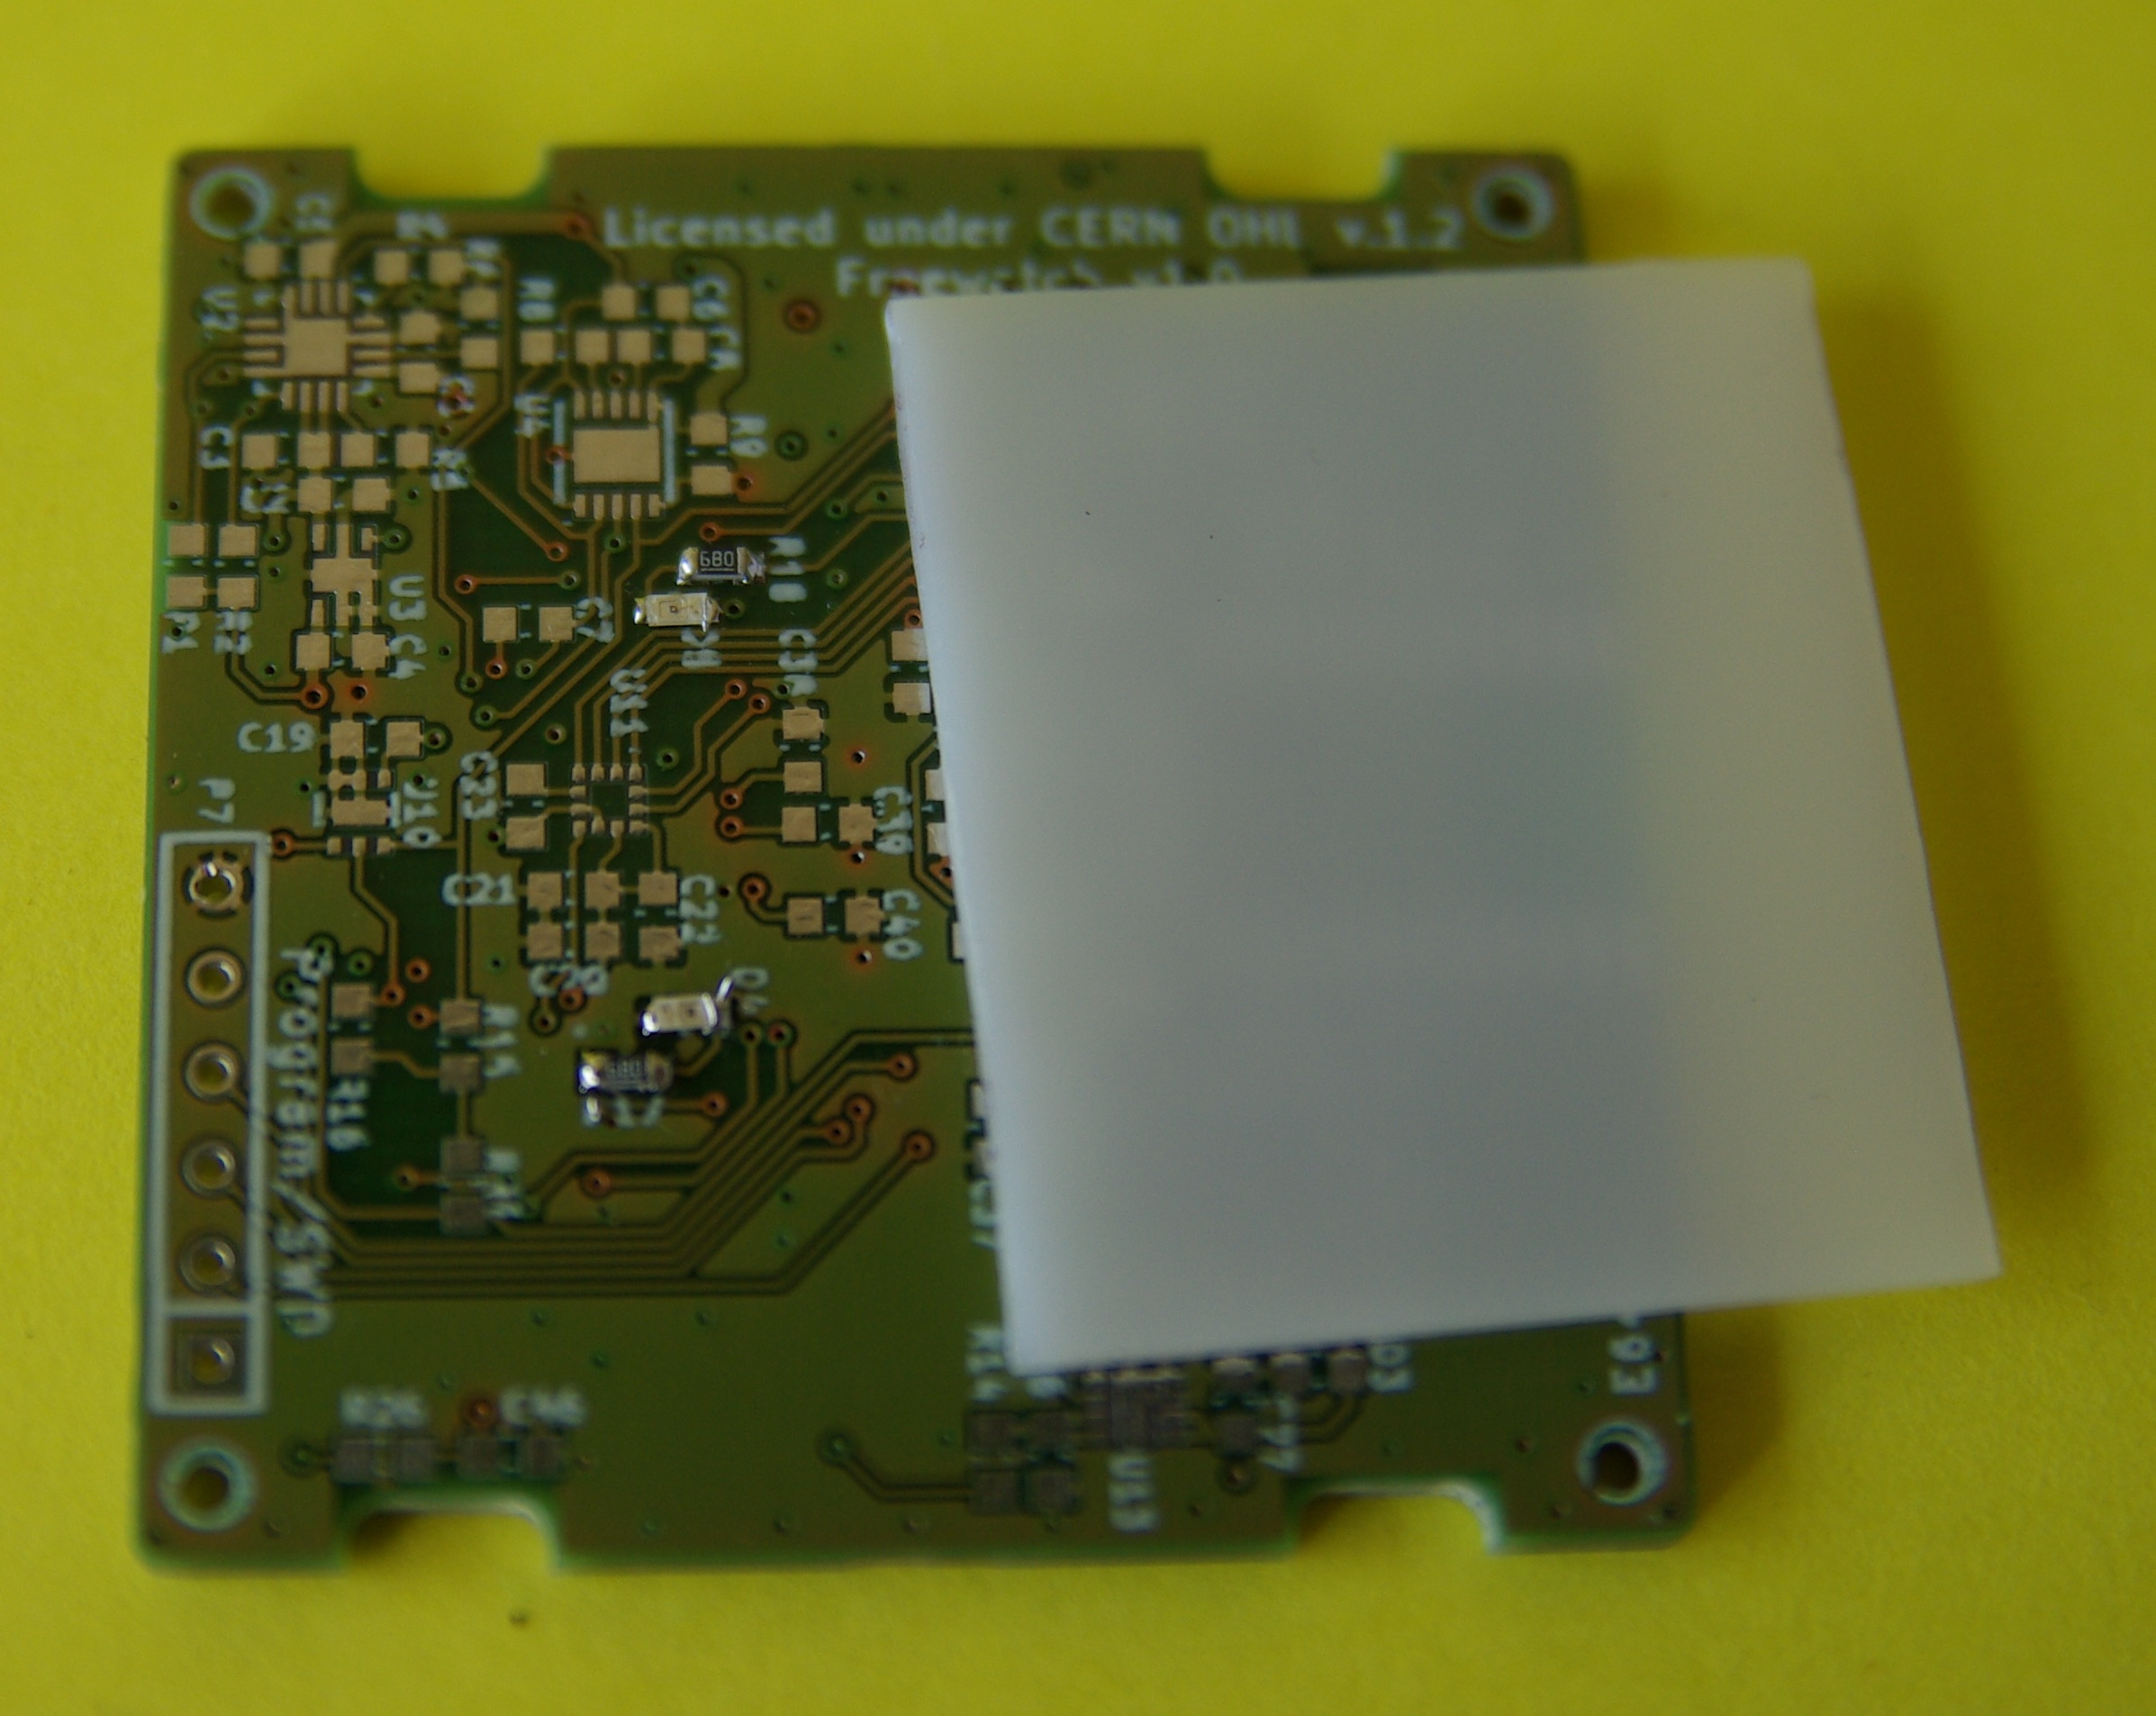
\includegraphics[height=4.5cm]{bl_led_off.eps}~
    \pause
    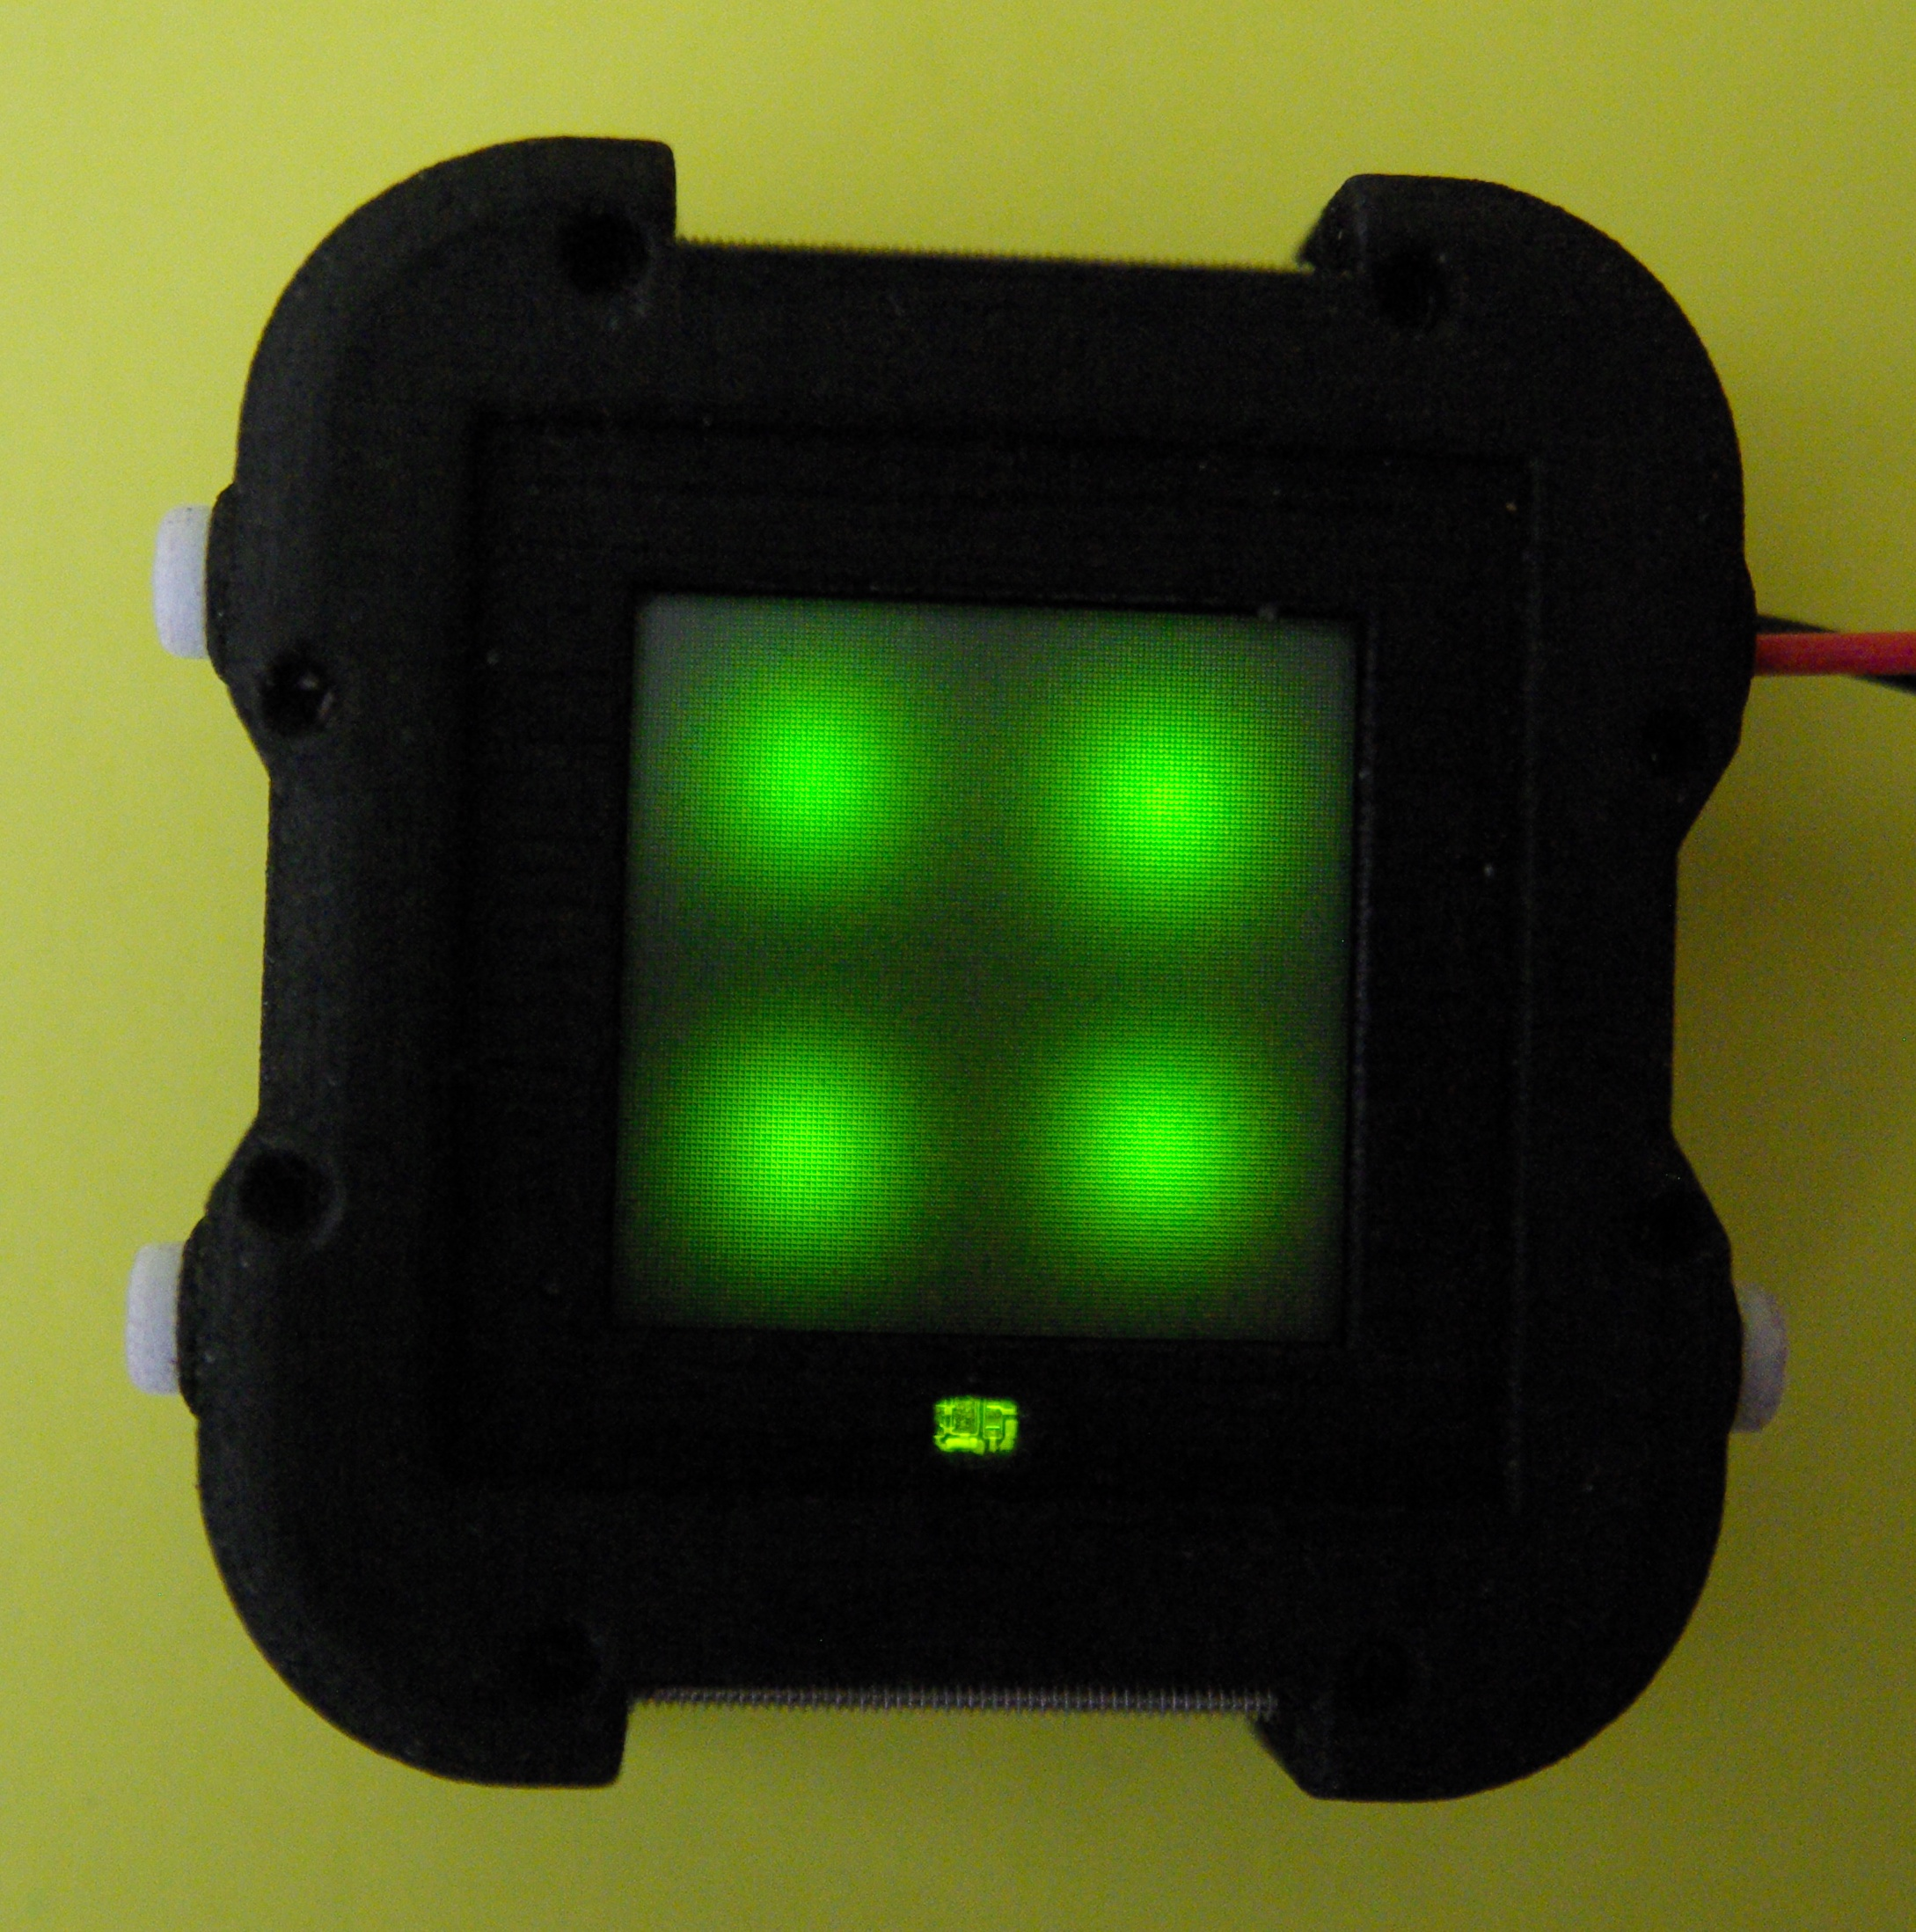
\includegraphics[height=4.5cm]{bl_led_on.eps}
  \end{center}

  \textbf{Not good!}

  \note[item]{We first though of putting a few LED on the top of the PCB}
  \note[item]{And a opaque piece of Plexiglas (~1mm) to diffuse the light}
  \note[item]{But as you can see on the picture, the light distribution is not uniform}

\end{frame}

%------------ FRAME --------------------------------------------------
\begin{frame}{Backlight}

  Second try: Recycled smartphone backlight

  \begin{center}
    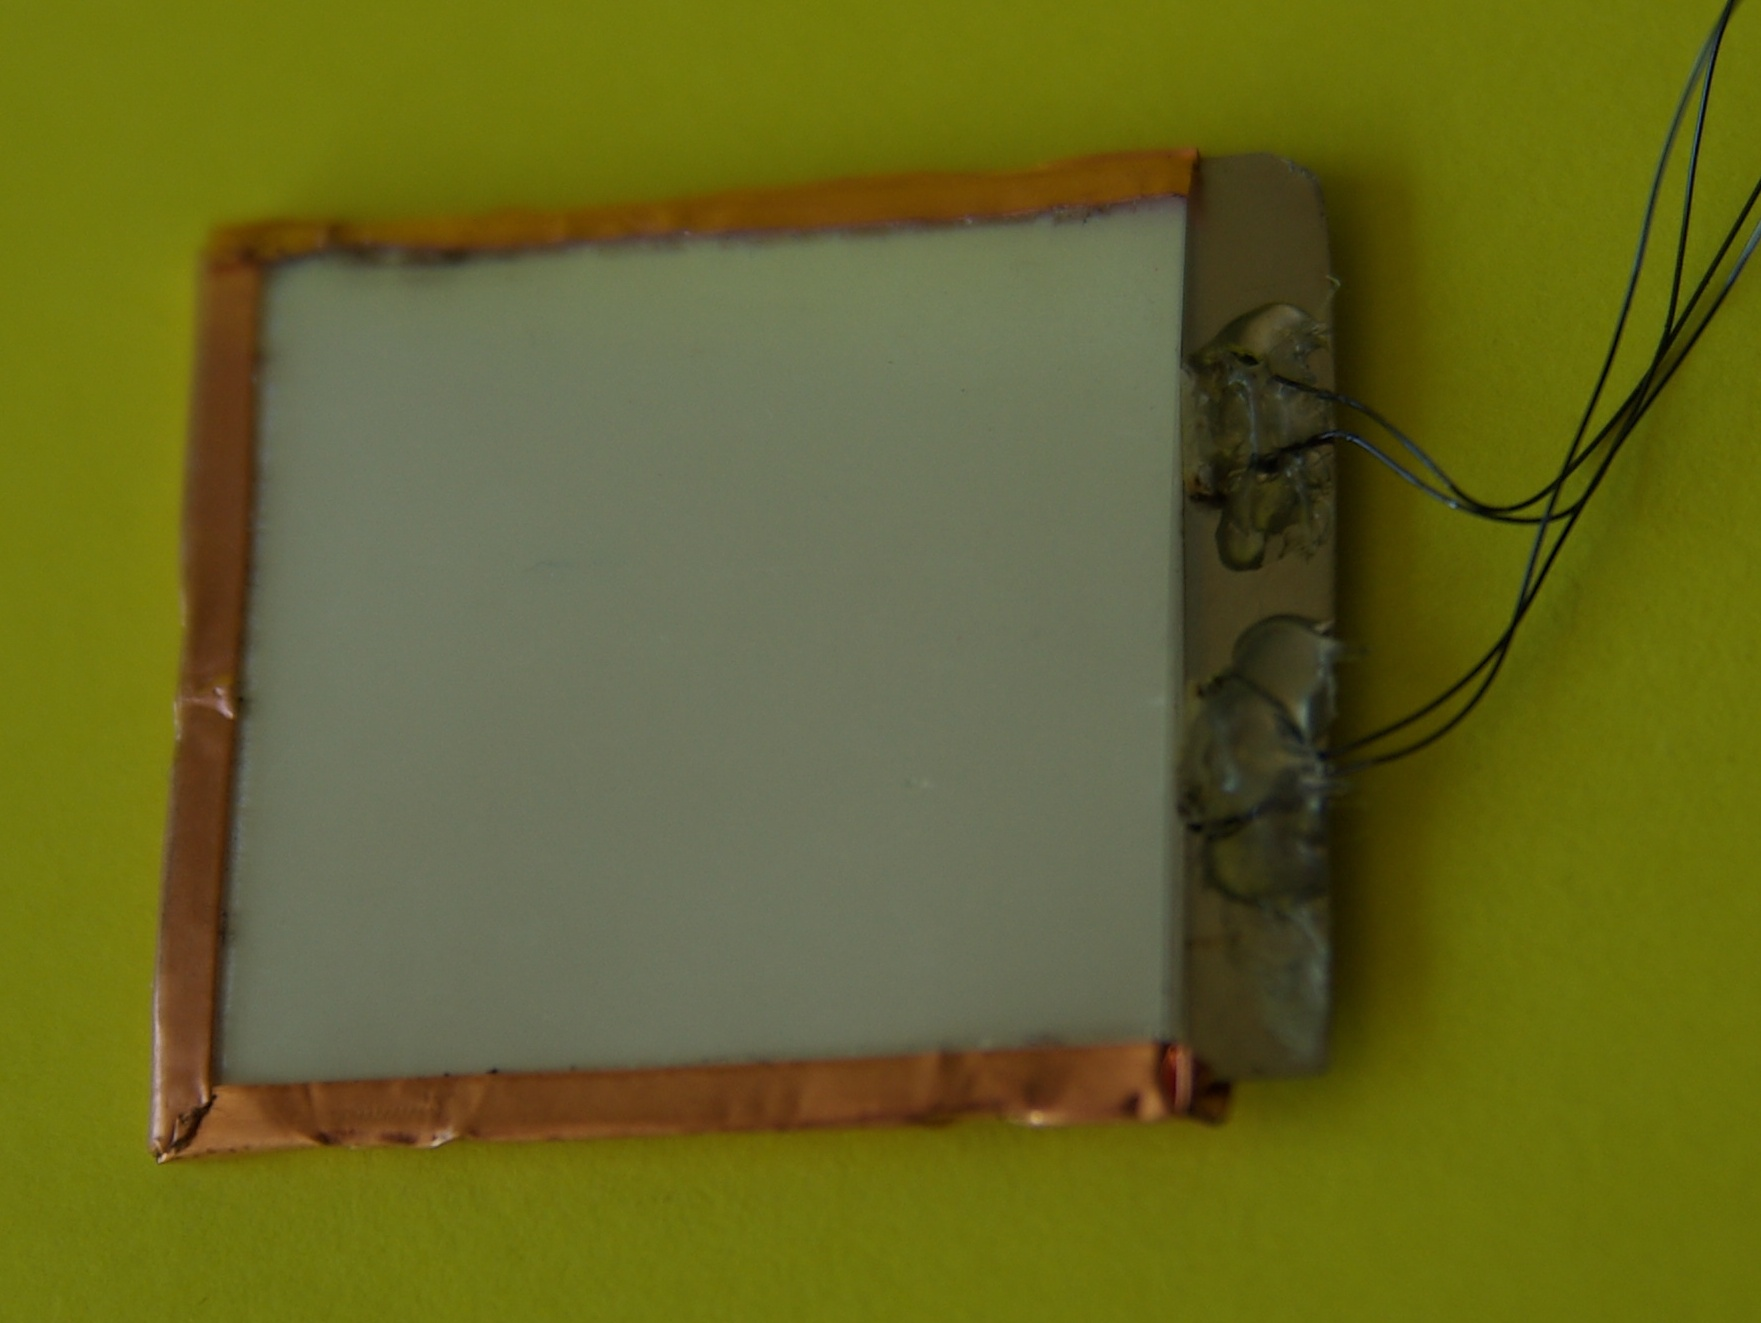
\includegraphics[height=4.5cm]{bl_smartphone_off.eps}~
    \pause
    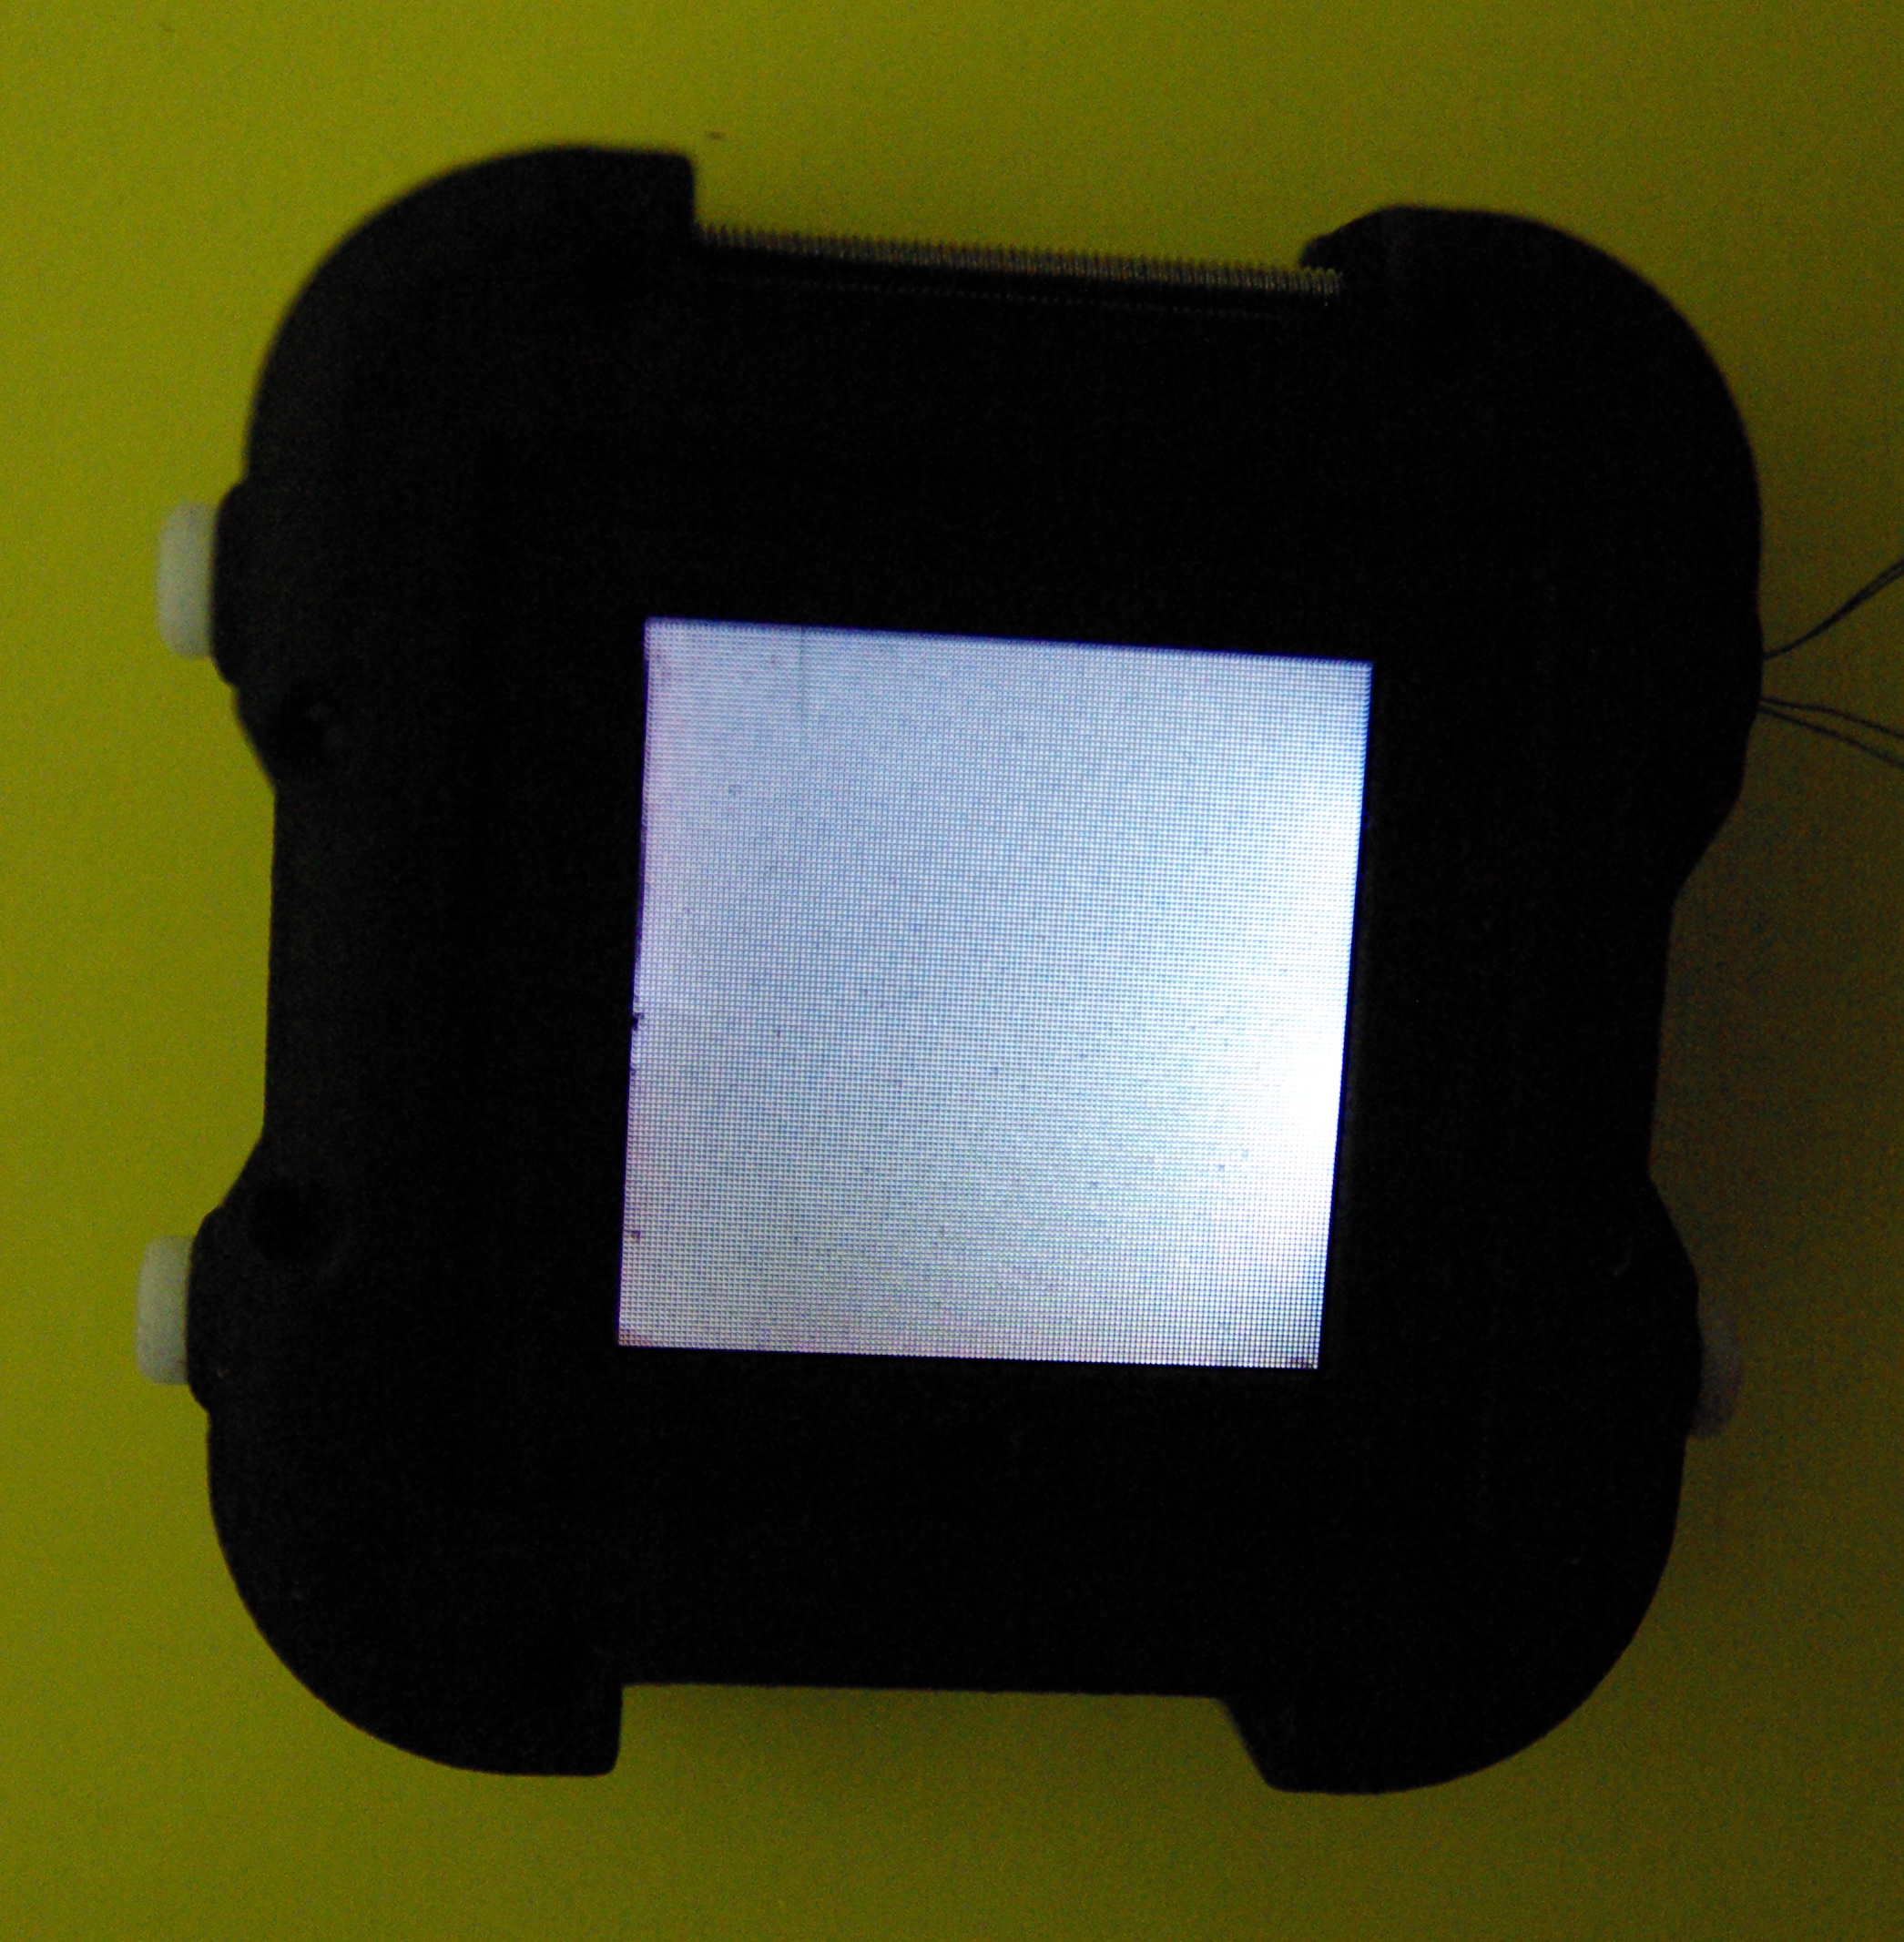
\includegraphics[height=4.5cm]{bl_smartphone_on.eps}
  \end{center}

  \textbf{Better, but...}

  \note[item]{Then we took the backlight of a broken smartphone screen and cut it to the right dimensions}
  \note[item]{As you can see, it work nicely, but...}
  \note[item]{It is not very suitable for production in series or to sell in a kit}

\end{frame}

%------------ FRAME --------------------------------------------------
\begin{frame}{Backlight}

  Current try: Custom-made module

  \begin{center}
    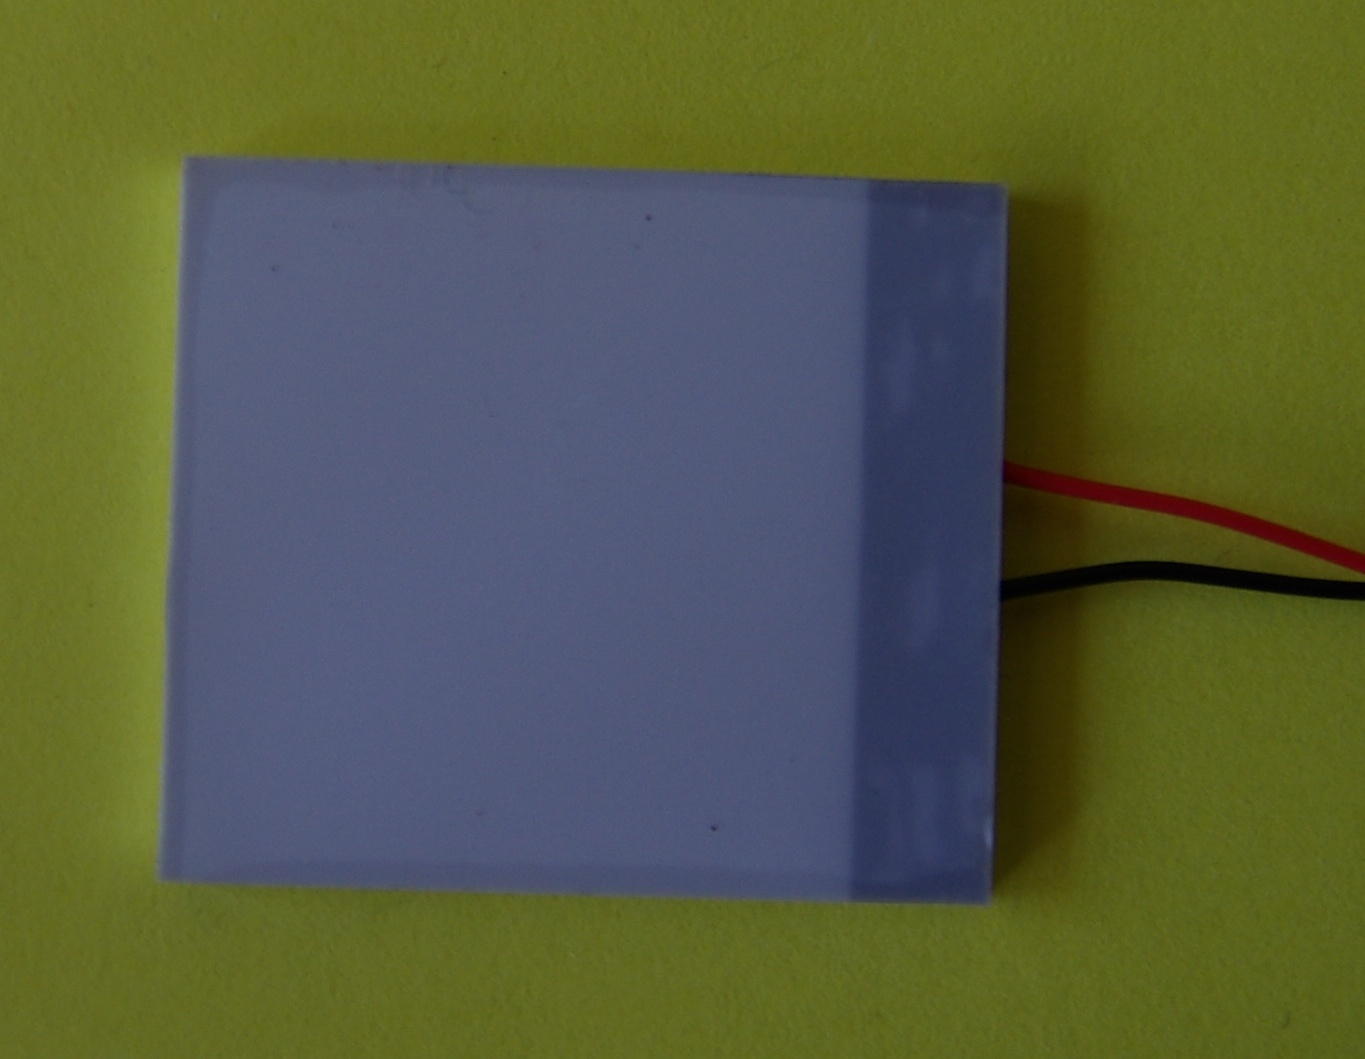
\includegraphics[height=4.5cm]{bl_custom_off.eps}~
    \pause
    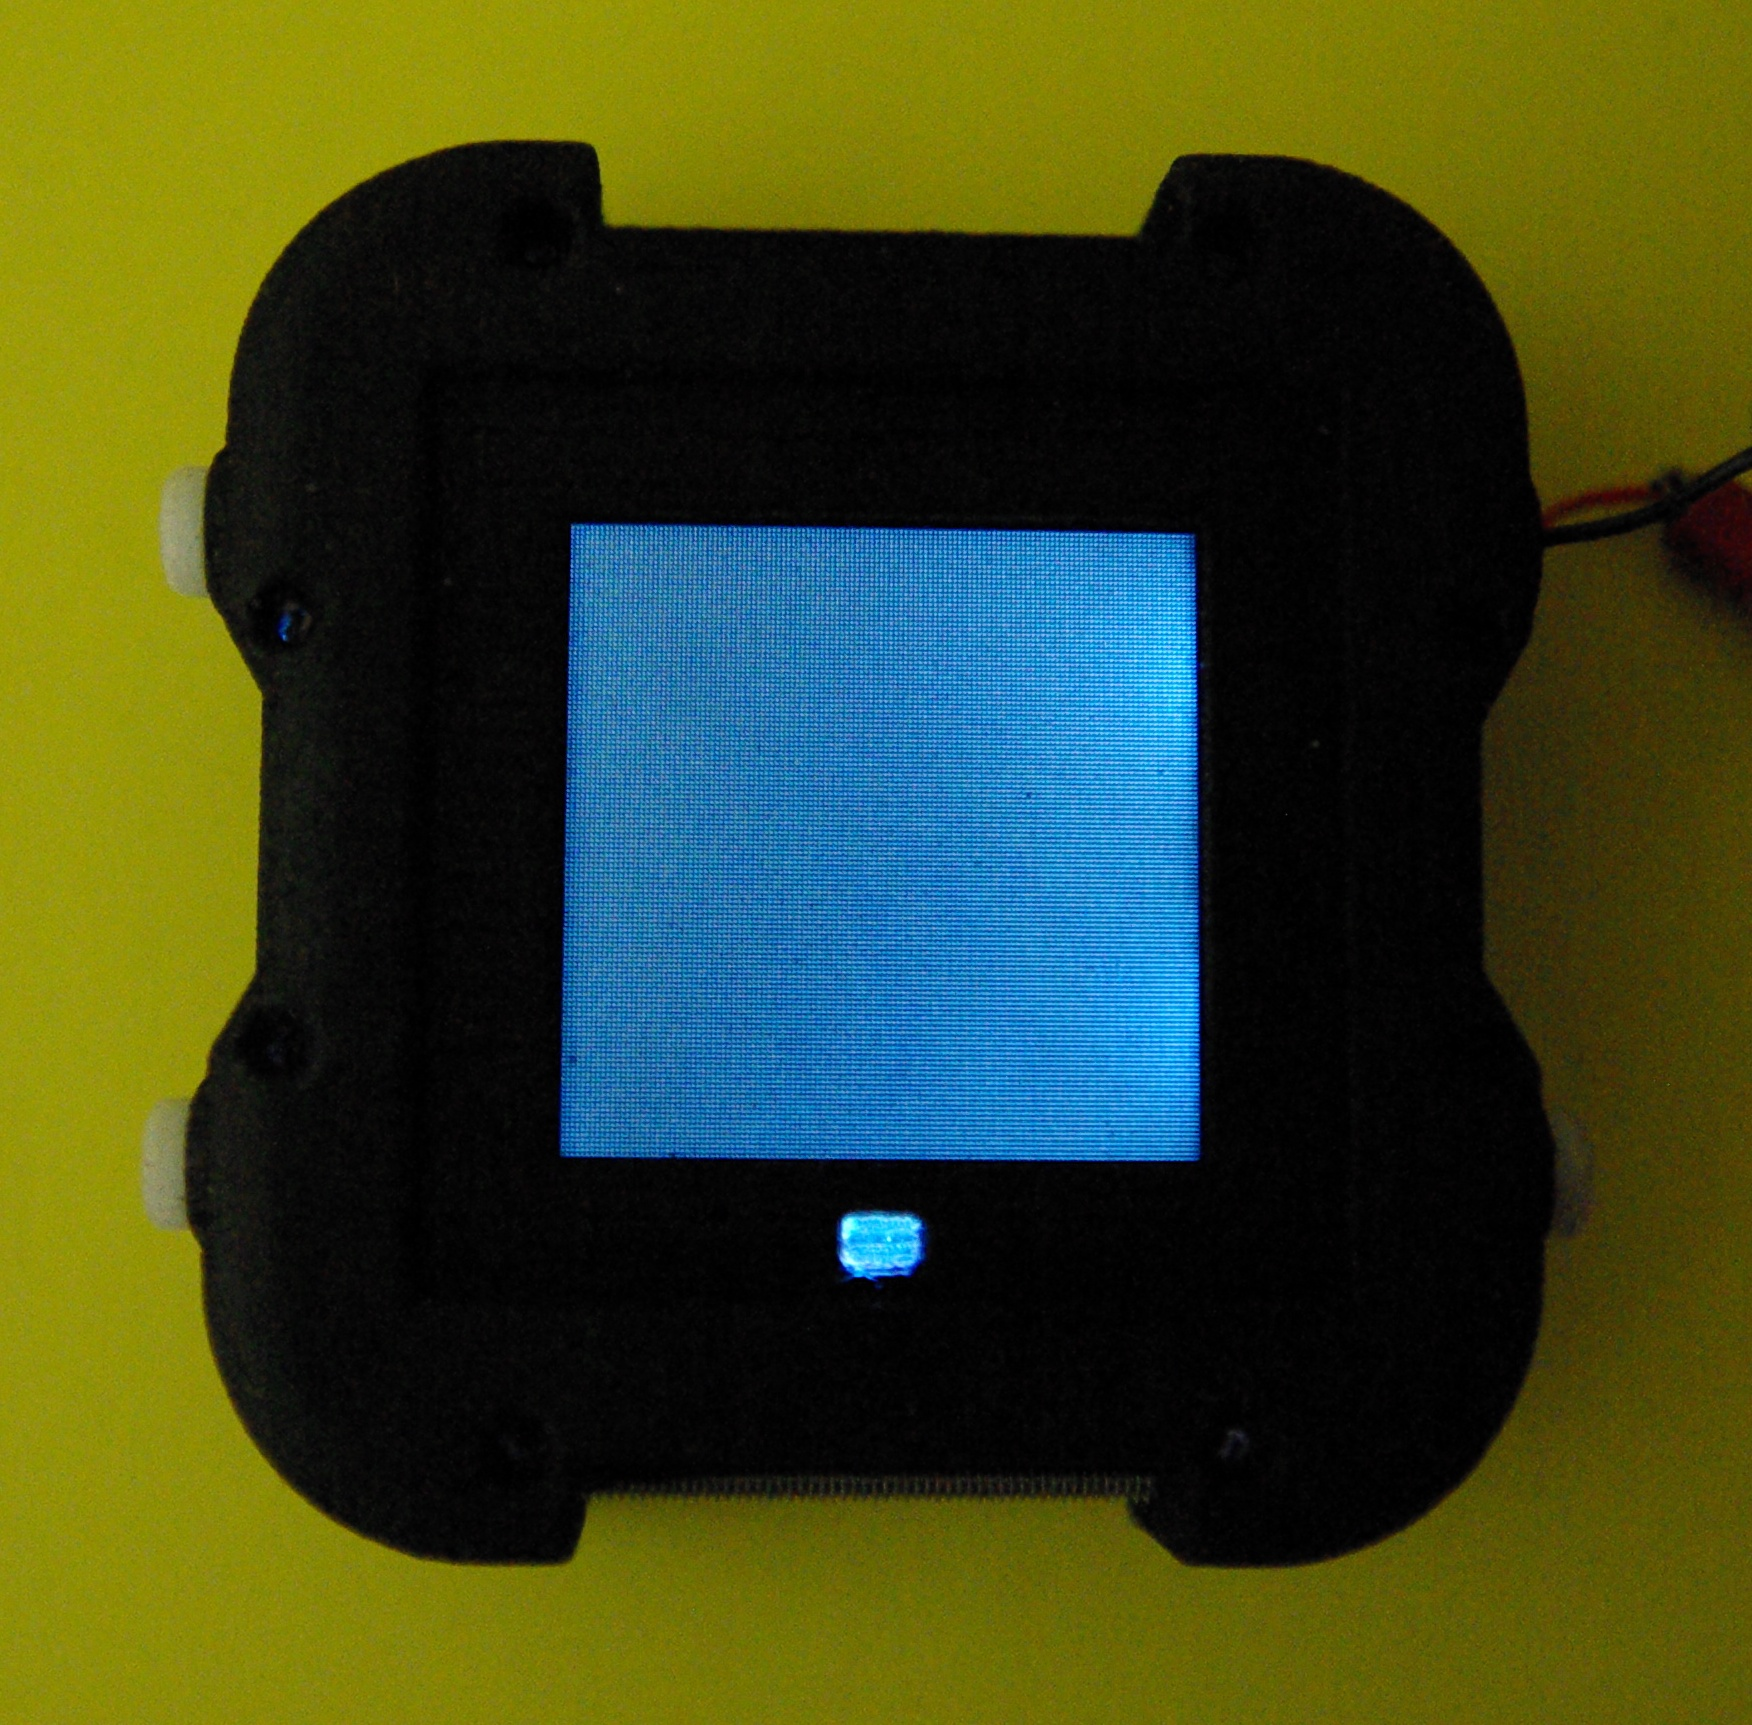
\includegraphics[height=4.5cm]{bl_custom_on.eps}
  \end{center}

  \textbf{The solution}

  \note[item]{We finally contacted many companies}
  \note[item]{And we found one with no Minimum Order Quantity of several thousands}
  \note[item]{You see here the first samples}
  \note[item]{There are surprisingly cheap, even for small quantity and have a good luminosity}
  \note[item]{(negative point, a bit thick compared to high-tech smartphones)}

\end{frame}

%------------ FRAME --------------------------------------------------
\begin{frame}{Mechanical design}

  CAD tool selection

  \begin{itemize}
  \item No mechanical engineer
  \item No experience in 3d design/printing
  \item Evaluate existing free CAD tools \\
    Freecad, OpenSCAD, Open CASCADE, ...
  \end{itemize}

  \pause
  Criteria

  \begin{itemize}
  \item Documentation, support
  \item User-friendliness, learning curve
  \end{itemize}

  \pause
  \begin{itemize}
  \item Decided to use \textbf{FreeCAD}
  \end{itemize}

  \begin{center}
    
\includegraphics[height=2cm]{freecad_logo.eps}
  \end{center}

  \note[item]{The biggest challenge in this project was probably the mechanical design of the case}
  \note[item]{Because we had no mechanical engineer in the team}
  \note[item]{And also no experience with 3d design and 3d printing}
  \note[item]{We evaluated the exiting free CAD tools [NEXT], based on:}
  \note[item]{The documentation, the support (forum)}
  \note[item]{Also the user-friendliness and the learning curve [NEXT]}
  \note[item]{In the end, we decided to use FreeCAD}

\end{frame}

%------------ FRAME --------------------------------------------------
\begin{frame}{Mechanical design}

  Full of new challenges
  \vskip 5mm

  \begin{itemize}
  \item Learning Freecad from scratch
  \item Design a watch case
  \item 3D printing
  \end{itemize}

  \pause
  \vskip 9mm
  \begin{center}
    It's time for a live demo!
  \end{center}

  \note[item]{We started to learn FreeCAD}
  \note[item]{A lot of online ressources (tutorial, forums, ...)}
  \note[item]{After leanring the basics, we had to design a watch case}
  \note[item]{And then learn about 3D printing}
  \note[item]{First looked for local companies}
  \note[item]{Then ear about online services like: Sculpteo, Shapeways}
  \note[item]{..[NEXT] time for a little live demo}
  %\note[item]{Learn Freecad from scratch = no mech engineer in the team, lots of online tutorials}
  %\note[item]{3D printing = didn't knew the domain, studied the main 3d printing services}
  %\note[item]{3D printing = every order was exiting, to see the result}
  %\note[item]{OR live demo at the end of mechanics section??}

\end{frame}


\begin{comment}

%------------ FRAME --------------------------------------------------
\begin{frame}{Mechanical design}

  \begin{itemize}
  \item Water-resistance (dropped for proto)
  \item Wrist-strap
  \end{itemize}

  \note[item]{Water-resistance = show, explain grove and rubber join idea}
  \note[item]{Wrist-strap = easy to get "nato" type wrist-strap, bought online}
  \note[item]{Might remove this slide?}

\end{frame}

\end{comment}


%------------ FRAME --------------------------------------------------
\begin{frame}{3D model}

  \begin{center}
    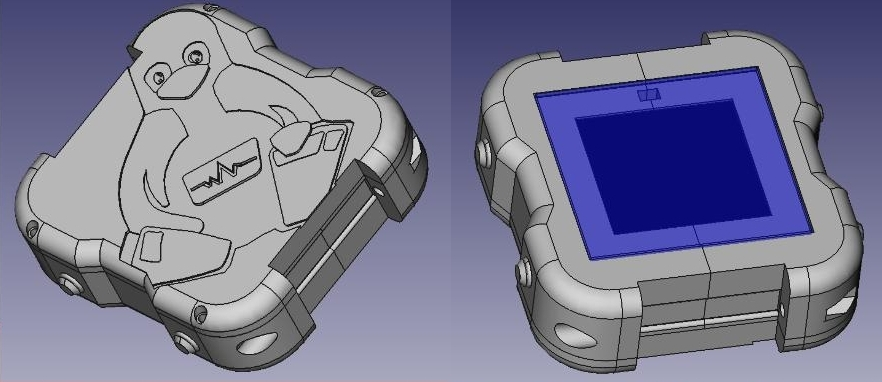
\includegraphics[height=4.8cm]{case-design-model.eps}
  \end{center}

  Making of movie (6 hours summarised in 5 minutes)
  \url{http://www.ohwr.org/projects/f-watch/wiki/Movies}

  \note[item]{This was just a quick example}
  \note[item]{You can imagine that drawing the watch case took lot more time}
  \note[item]{You can see here the final result}
  \note[item]{If you are interested, a 5 min movie is available on our website}

\end{frame}

%------------ FRAME --------------------------------------------------
\begin{frame}{First 3D print}

  \begin{itemize}
  \item Fused plastic material - Low cost 3D printer
  \end{itemize}

  \begin{center}
    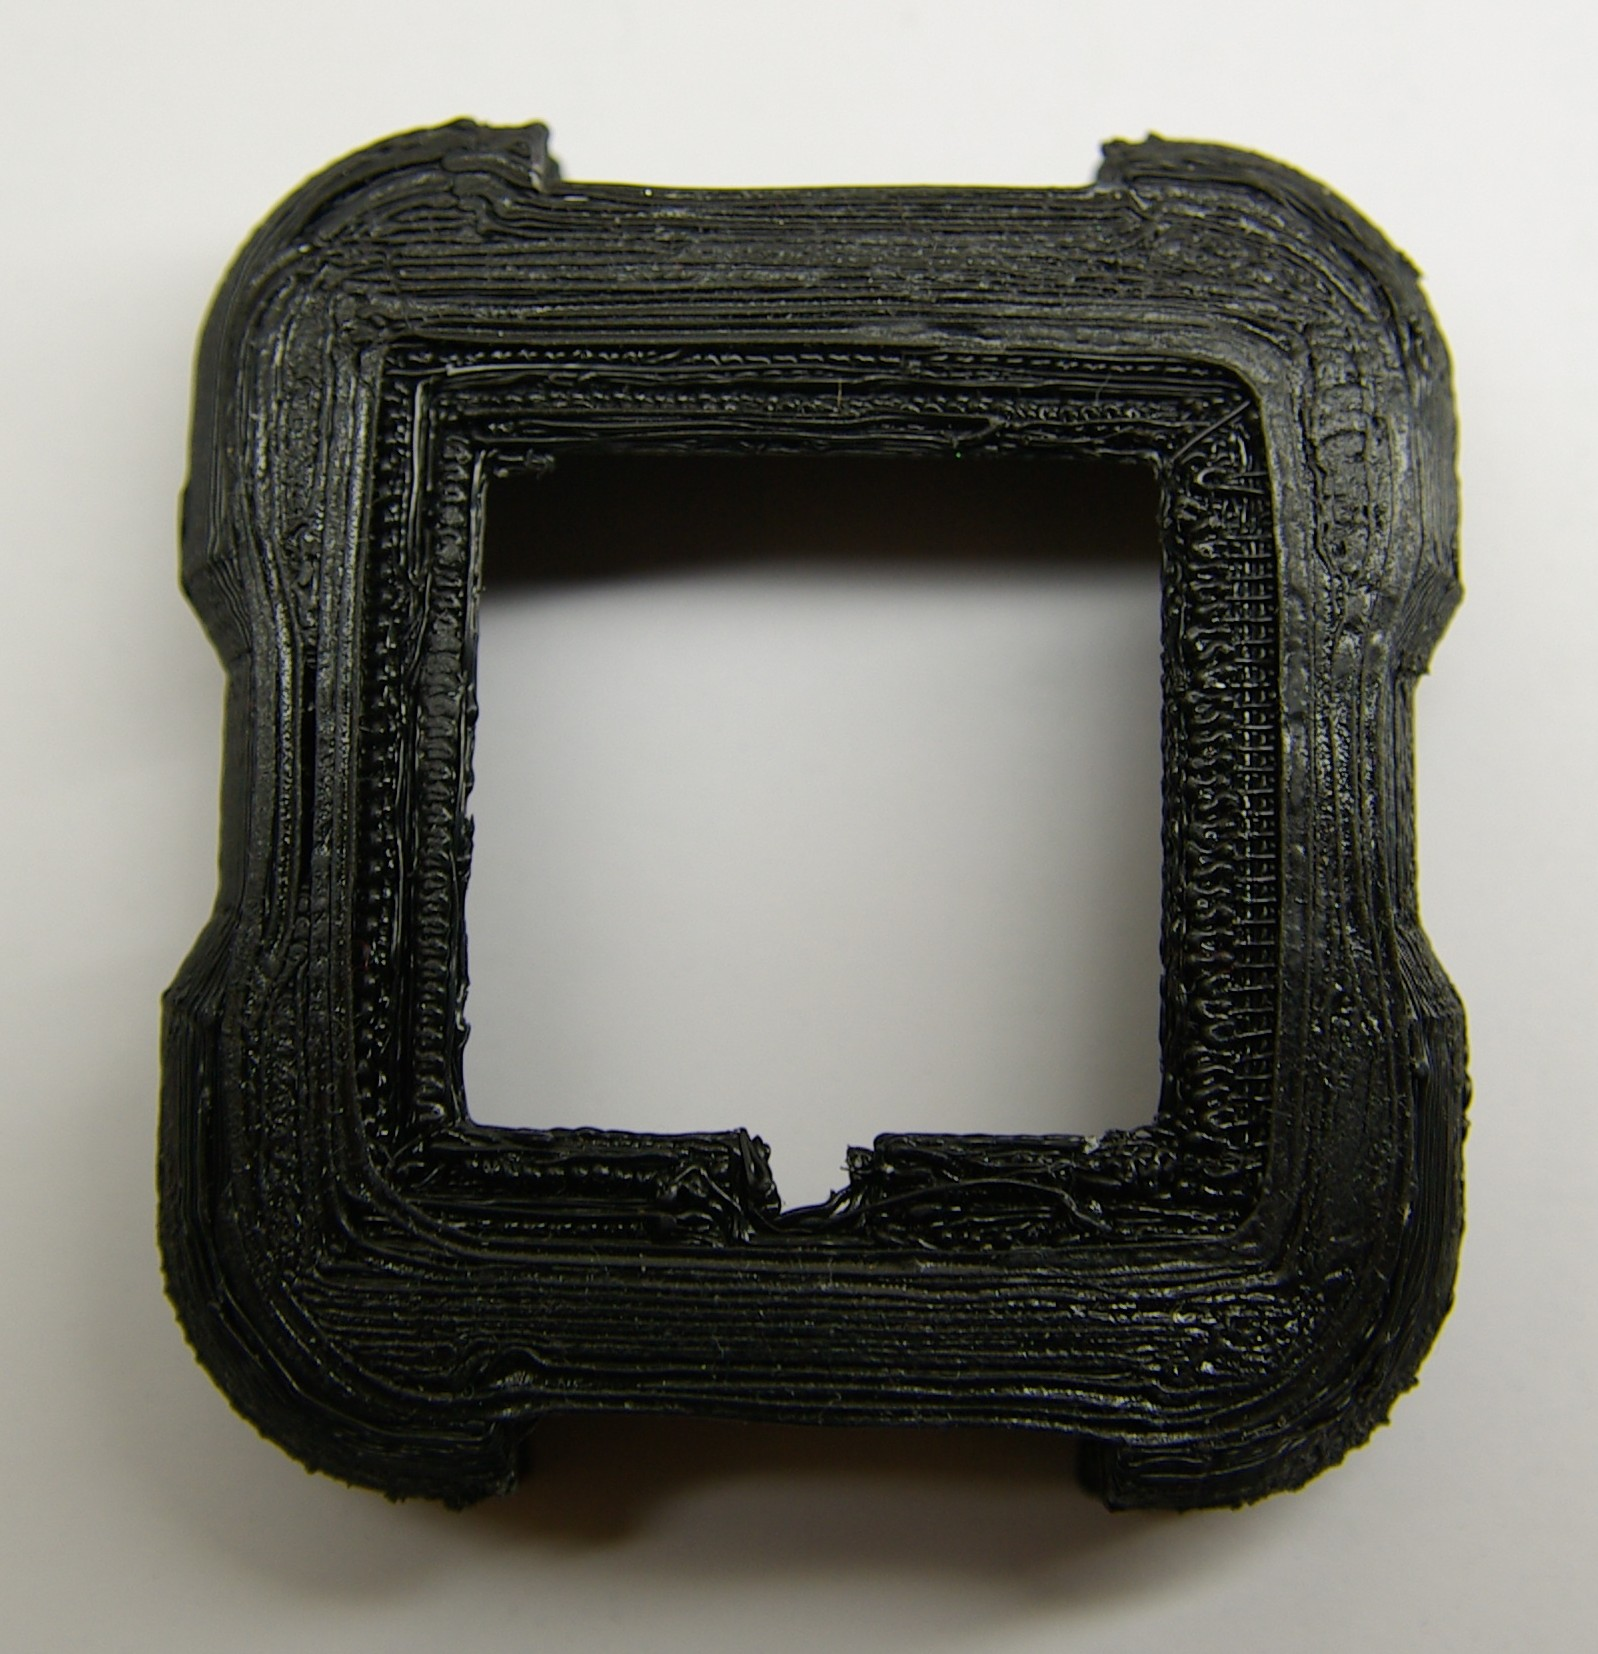
\includegraphics[height=5cm]{case-design-print-v1.eps}~
    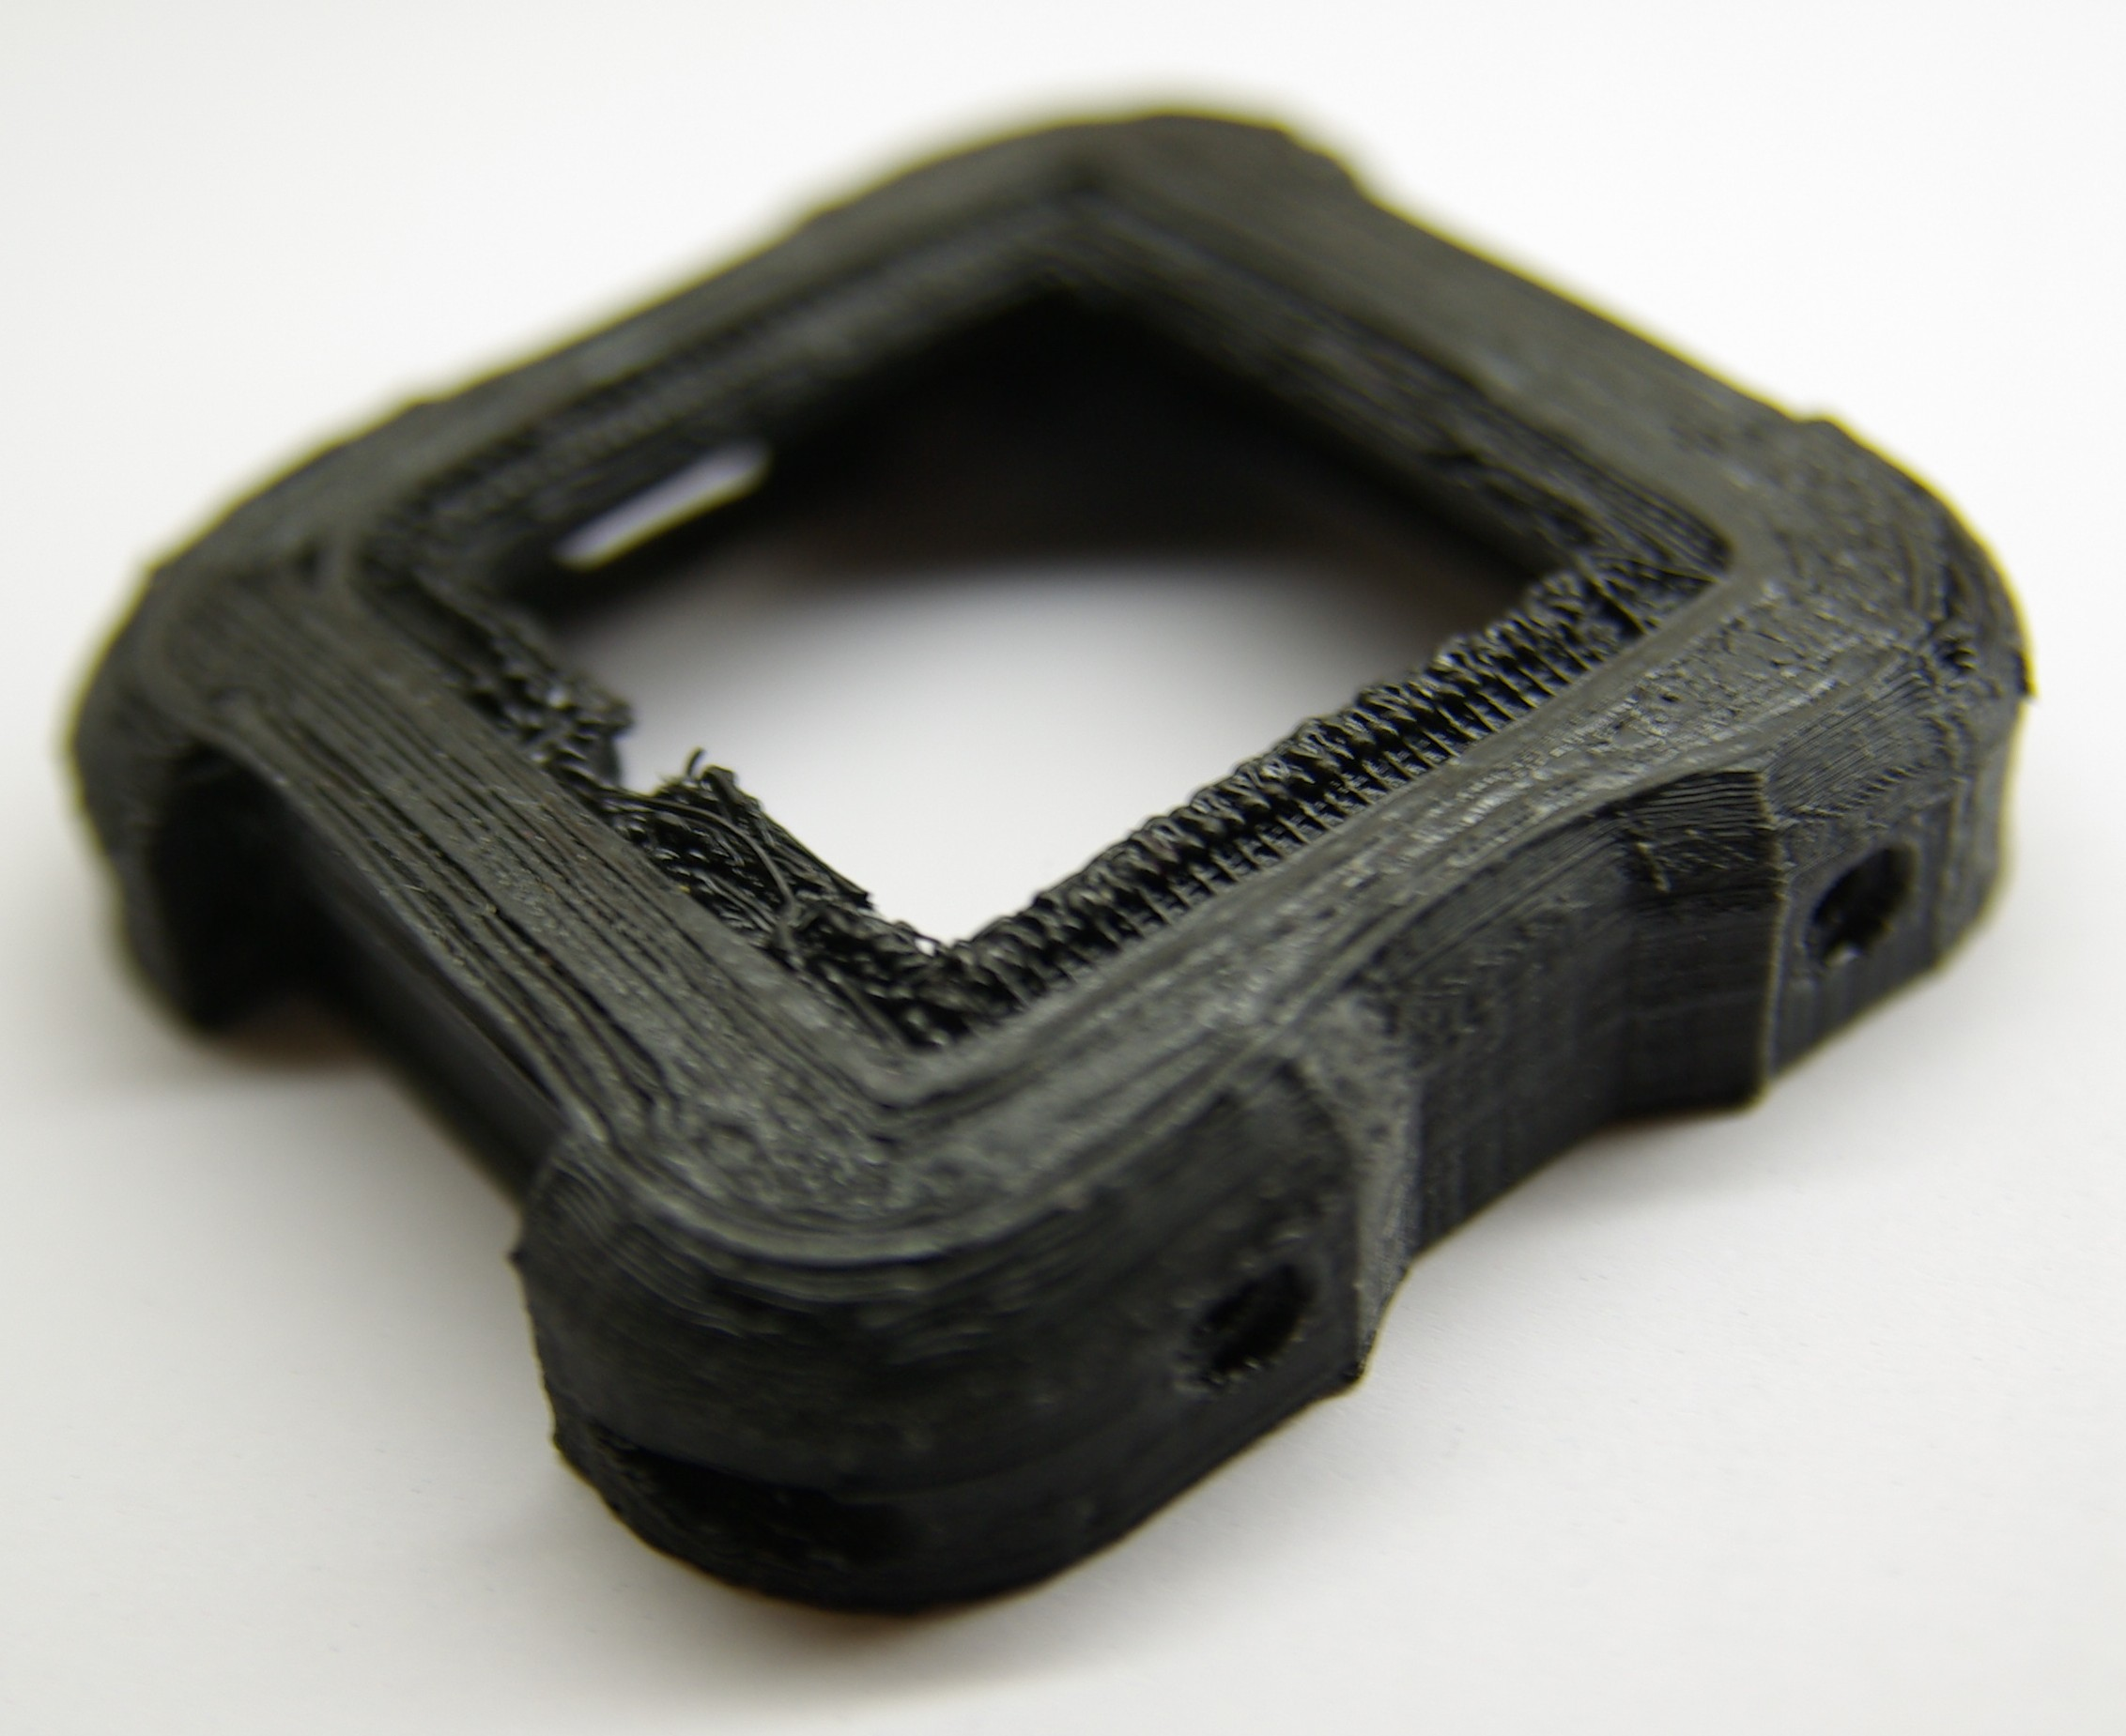
\includegraphics[height=5cm]{case-design-print-v1-2.eps}
  \end{center}

  %\note[item]{FDM = Fused deposition modeling}
  \note[item]{Very first print, done with a cheap 3D printer}
  \note[item]{Poor quality}
  \note[item]{Too low resolution}

\end{frame}

%------------ FRAME --------------------------------------------------
\begin{frame}{Second 3D print}

  \begin{itemize}
  \item Plastic material (powder)
  \end{itemize}

  \begin{center}
    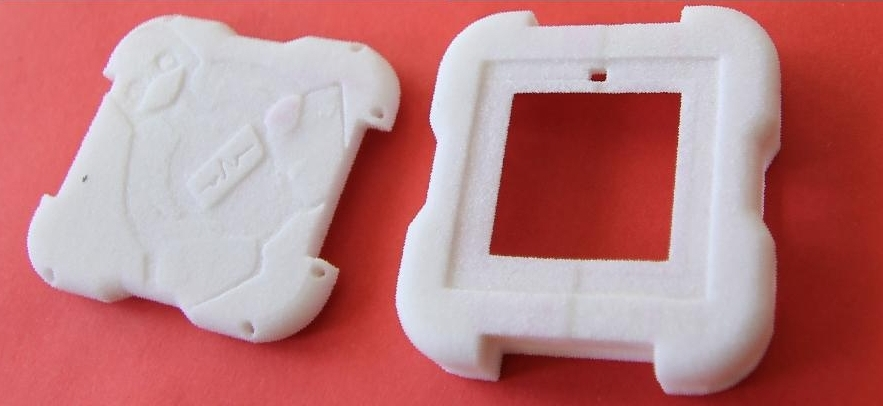
\includegraphics[height=5cm]{case-design-print-v2.eps}
  \end{center}

  \note[item]{The second was better}
  \note[item]{The resolution was good}
  \note[item]{But not smooth}
  \note[item]{And not water-tight}

\end{frame}

%------------ FRAME --------------------------------------------------
\begin{frame}{Third 3D print}

  \begin{itemize}
  \item Resin material
  \end{itemize}

  \begin{center}
    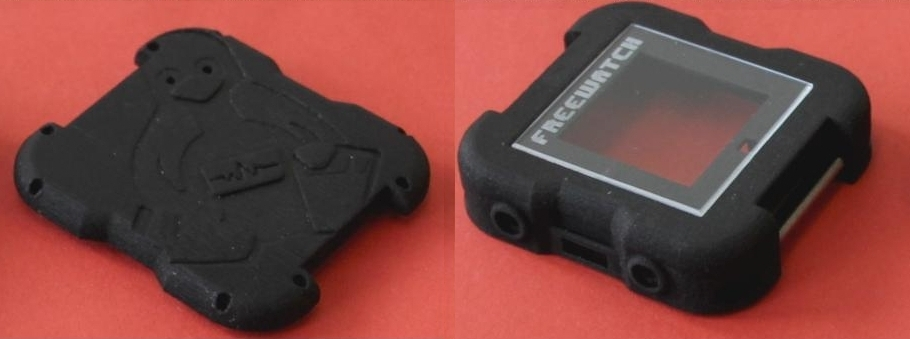
\includegraphics[height=4.1cm]{case-design-print-v3.eps}
  \end{center}

  \note[item]{Then we tried another material, a resin}
  \note[item]{Supposed to be water-resistant}
  \note[item]{Smooth surface}
  \note[item]{We realised that the screw supposed to hold the two parts of the case together were not holding well!}

\end{frame}

%------------ FRAME --------------------------------------------------
\begin{frame}{Forth 3D print}

  \begin{itemize}
  \item Resin material
  \item Improved case parts fastening
  \end{itemize}

  \begin{center}
    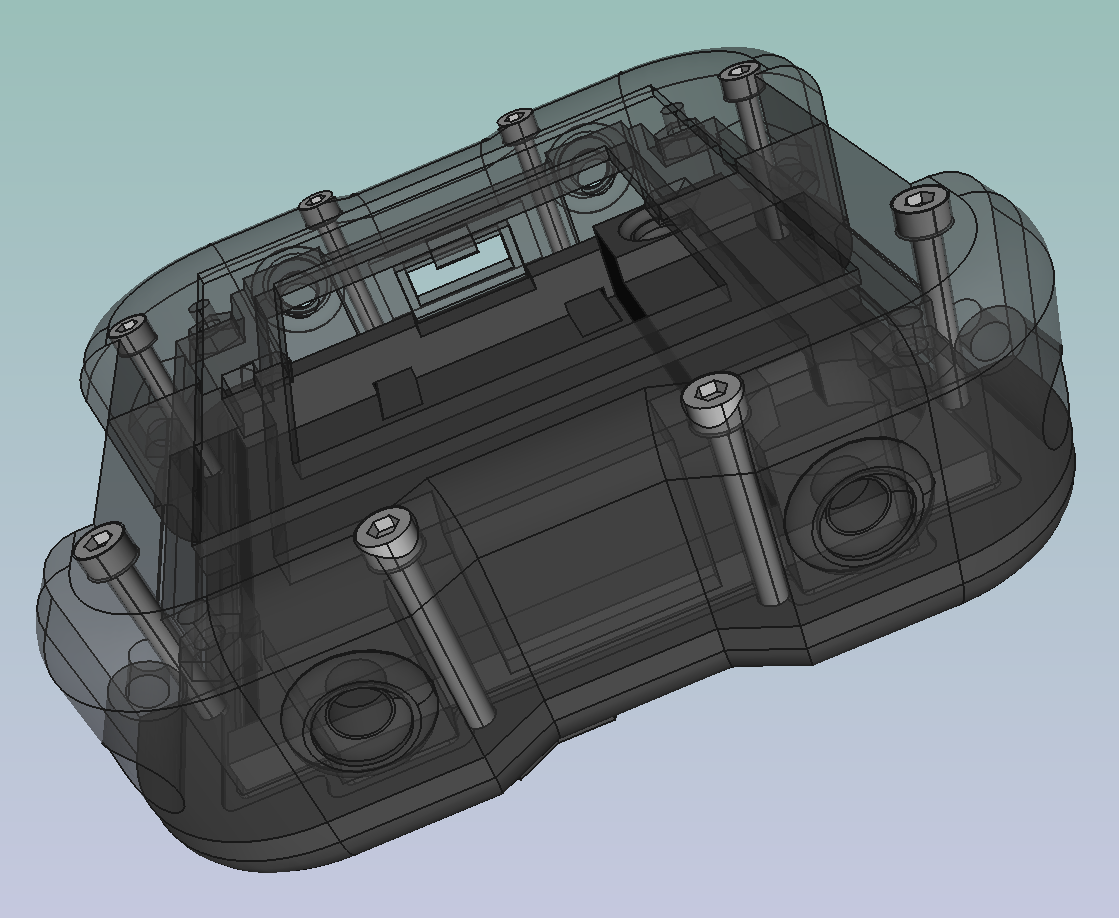
\includegraphics[height=4.5cm]{case_new_screws-2.eps}~
    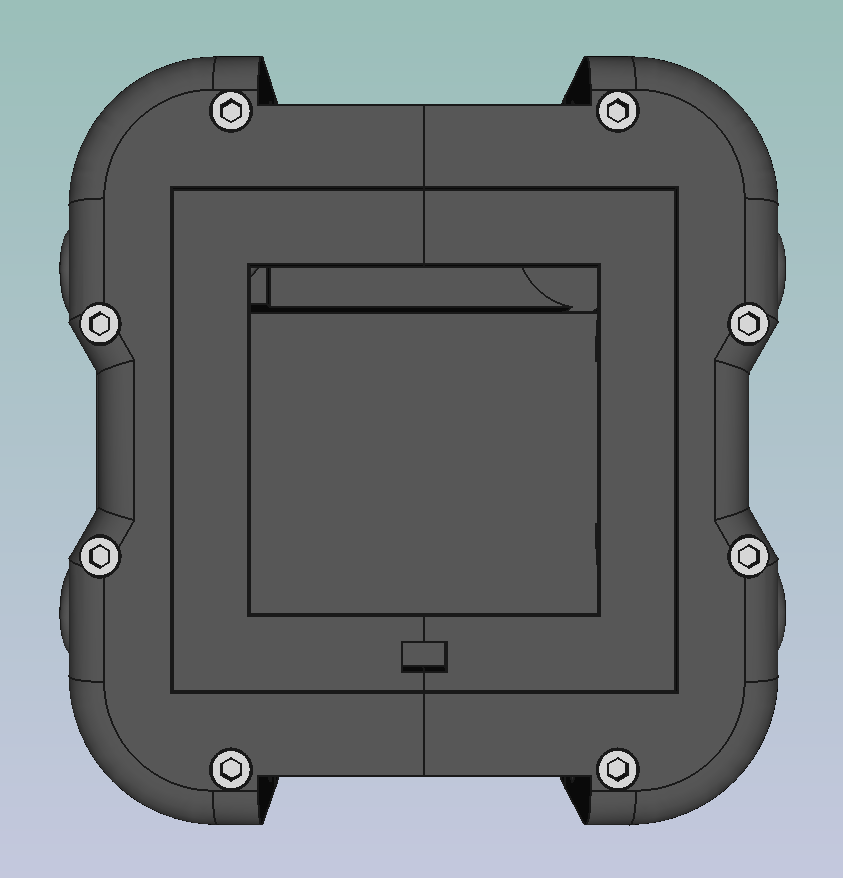
\includegraphics[height=4.5cm]{case_new_screws-3.eps}
  \end{center}

 % \note{Talk about improvements to be done?? Water-resistance}
  \note[item]{So we modified the model and put the screws through the top of the case}
  \note[item]{And we have some nuts in the bottom part}
  \note[item]{This way, the case parts are really holding well}

\end{frame}

%------------ FRAME --------------------------------------------------
\begin{frame}{Mechanical design}

  The buttons

  \begin{center}
    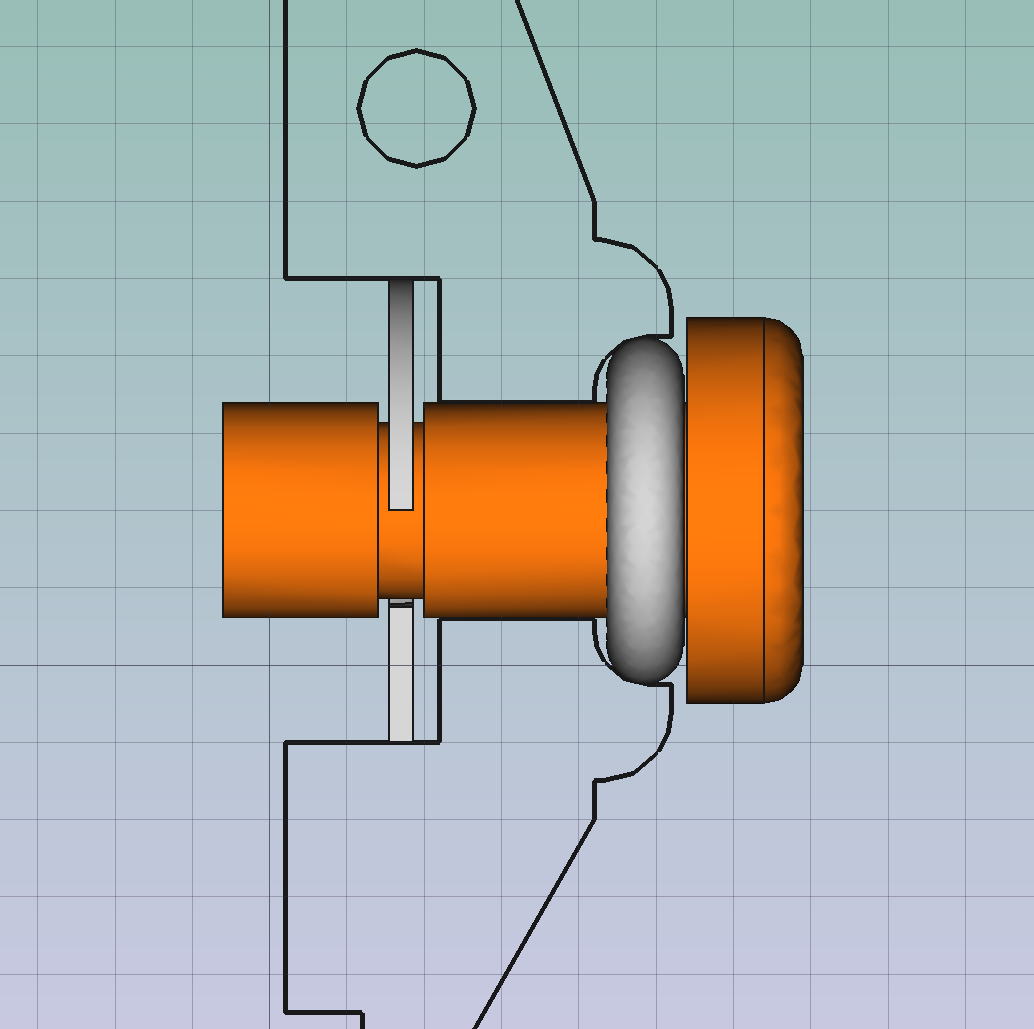
\includegraphics[height=4.5cm]{button_cross-section.eps}~
    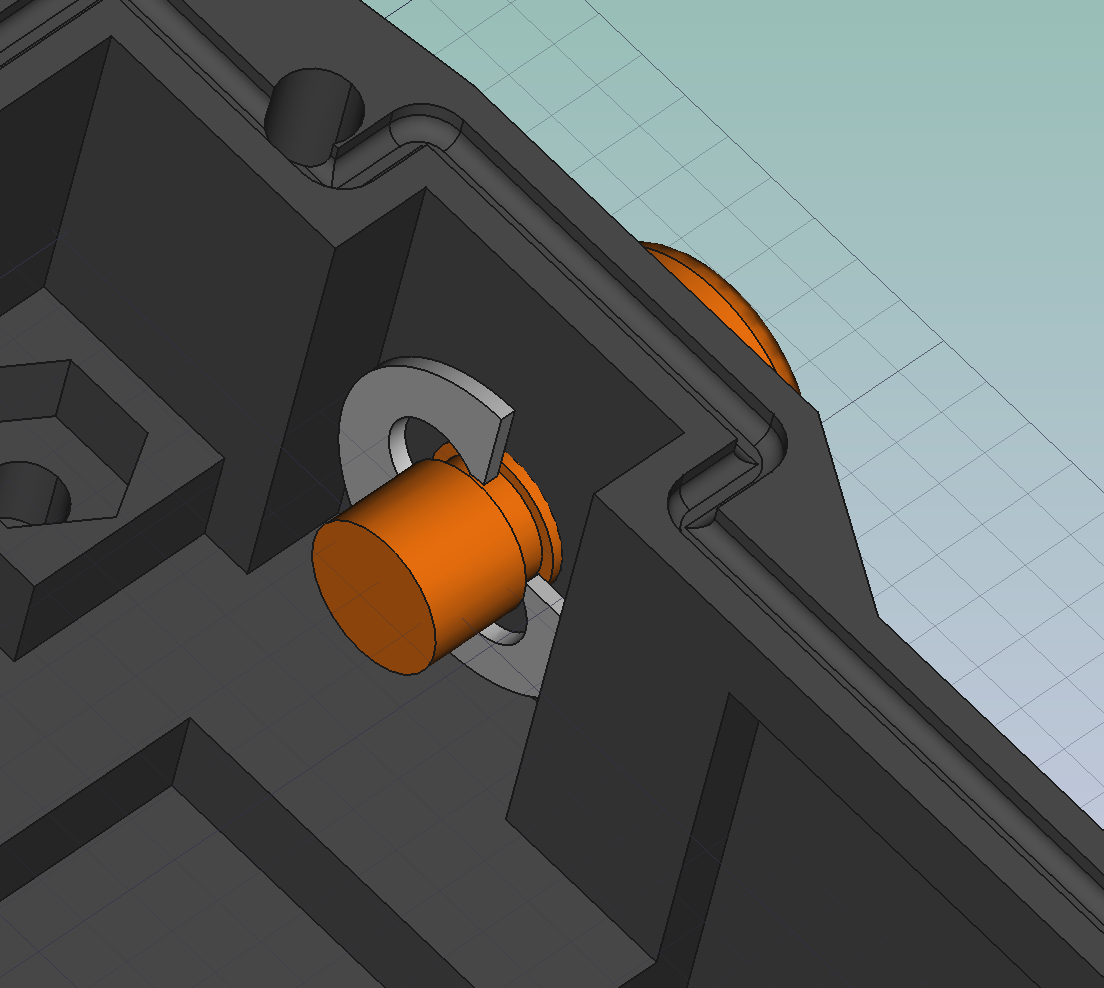
\includegraphics[height=4.5cm]{button_circlip.eps}
  \end{center}

  %\note[item]{maybe some hand drawing of our ideas?}
  \note[item]{Another challenge was the buttons}
  \note[item]{First we though of using small springs to push the button back, but to complex in the end.}
  \note[item]{Did some tests with the switch $\rightarrow$ the button is going back in place}
  \note[item]{Oring for water-resistance}
  \note[item]{Circlip to hold the button in place}

\end{frame}



%#####################################################################
%############ SECTION ################################################
\section{Building a watch}

\subsection*{} % dummy subsection to display dots

%------------ FRAME --------------------------------------------------
\begin{frame}{Building the watch}

  %Components procurement \& tools

  \begin{itemize}
  \item Buy electronics/mechanical components
  \item Download circuit Gerber files and order PCB
  \item Assemble the board
  \item Download case/button models and order 3D print
  \item Buy/build a programmer (bootloader)
  %\item Soldering paste
  %\item Hot-air station or oven
  %\item Soldering iron (finish/re-work)
  \item Optional: Milling machine (Plexiglas)
  \end{itemize}

  \begin{center}
    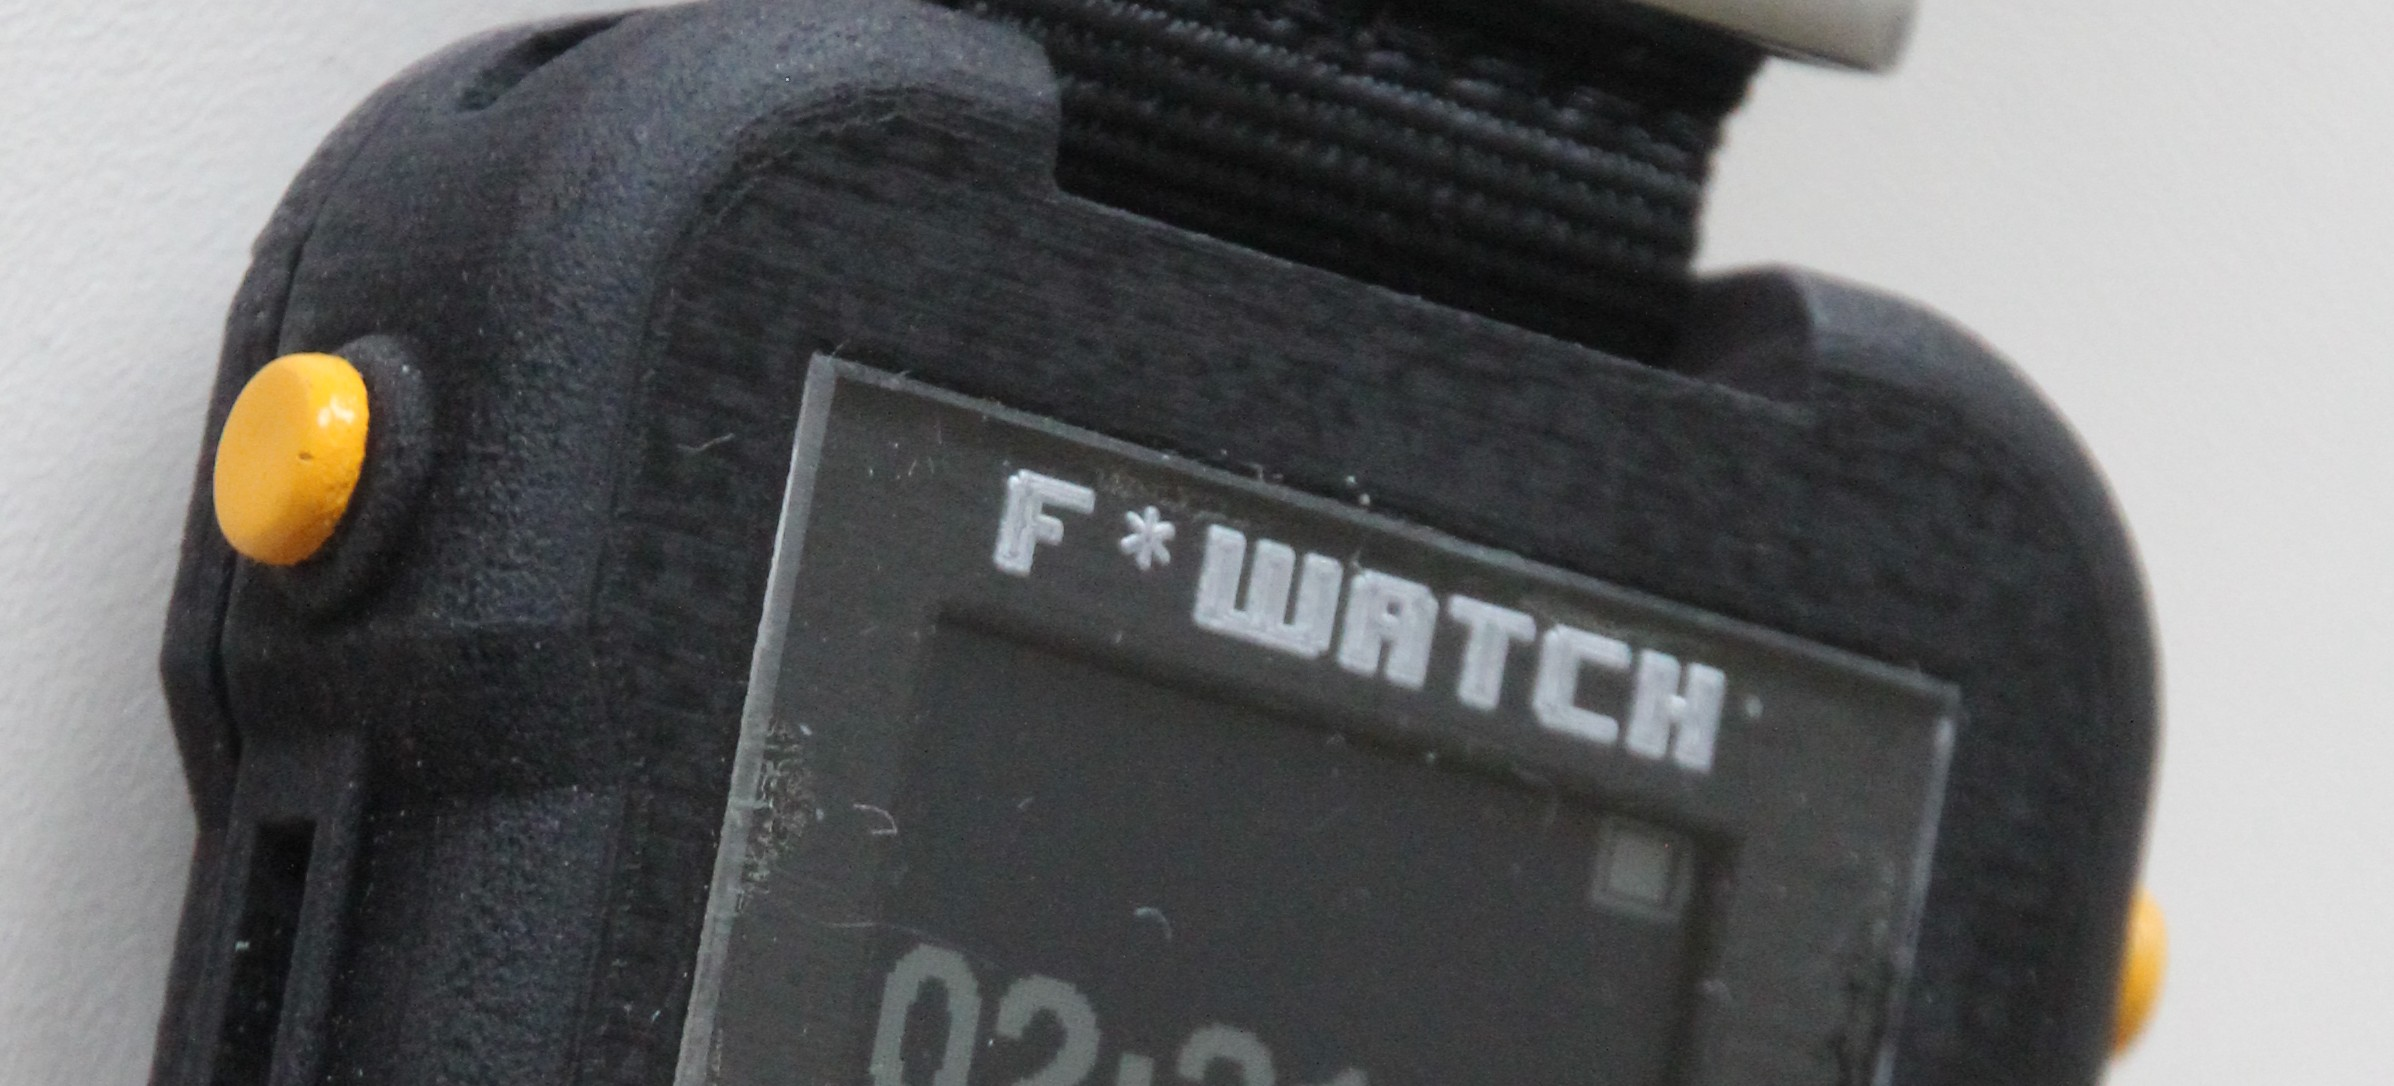
\includegraphics[height=2cm]{plexiglass.eps}
  \end{center}

  %\note[item]{I want to build this watch, what should I do?}
  \note[item]{Components available from main suppliers}
  \note[item]{Programmer to write the bootloader}
  \note[item]{}
  %\note[item]{Talk about BGA soldering on the next slide!}

\end{frame}


\begin{comment}
%------------ FRAME --------------------------------------------------
\begin{frame}{Building the watch}

  PCB assembly

  \begin{itemize}
  \item Stencils (ordered with PCB)
  \item Soldering paste
  \item Components placed by hand
  \item Script to generate placement pdf
  \item Soldered with hot-air station
  \end{itemize}

  \begin{center}
    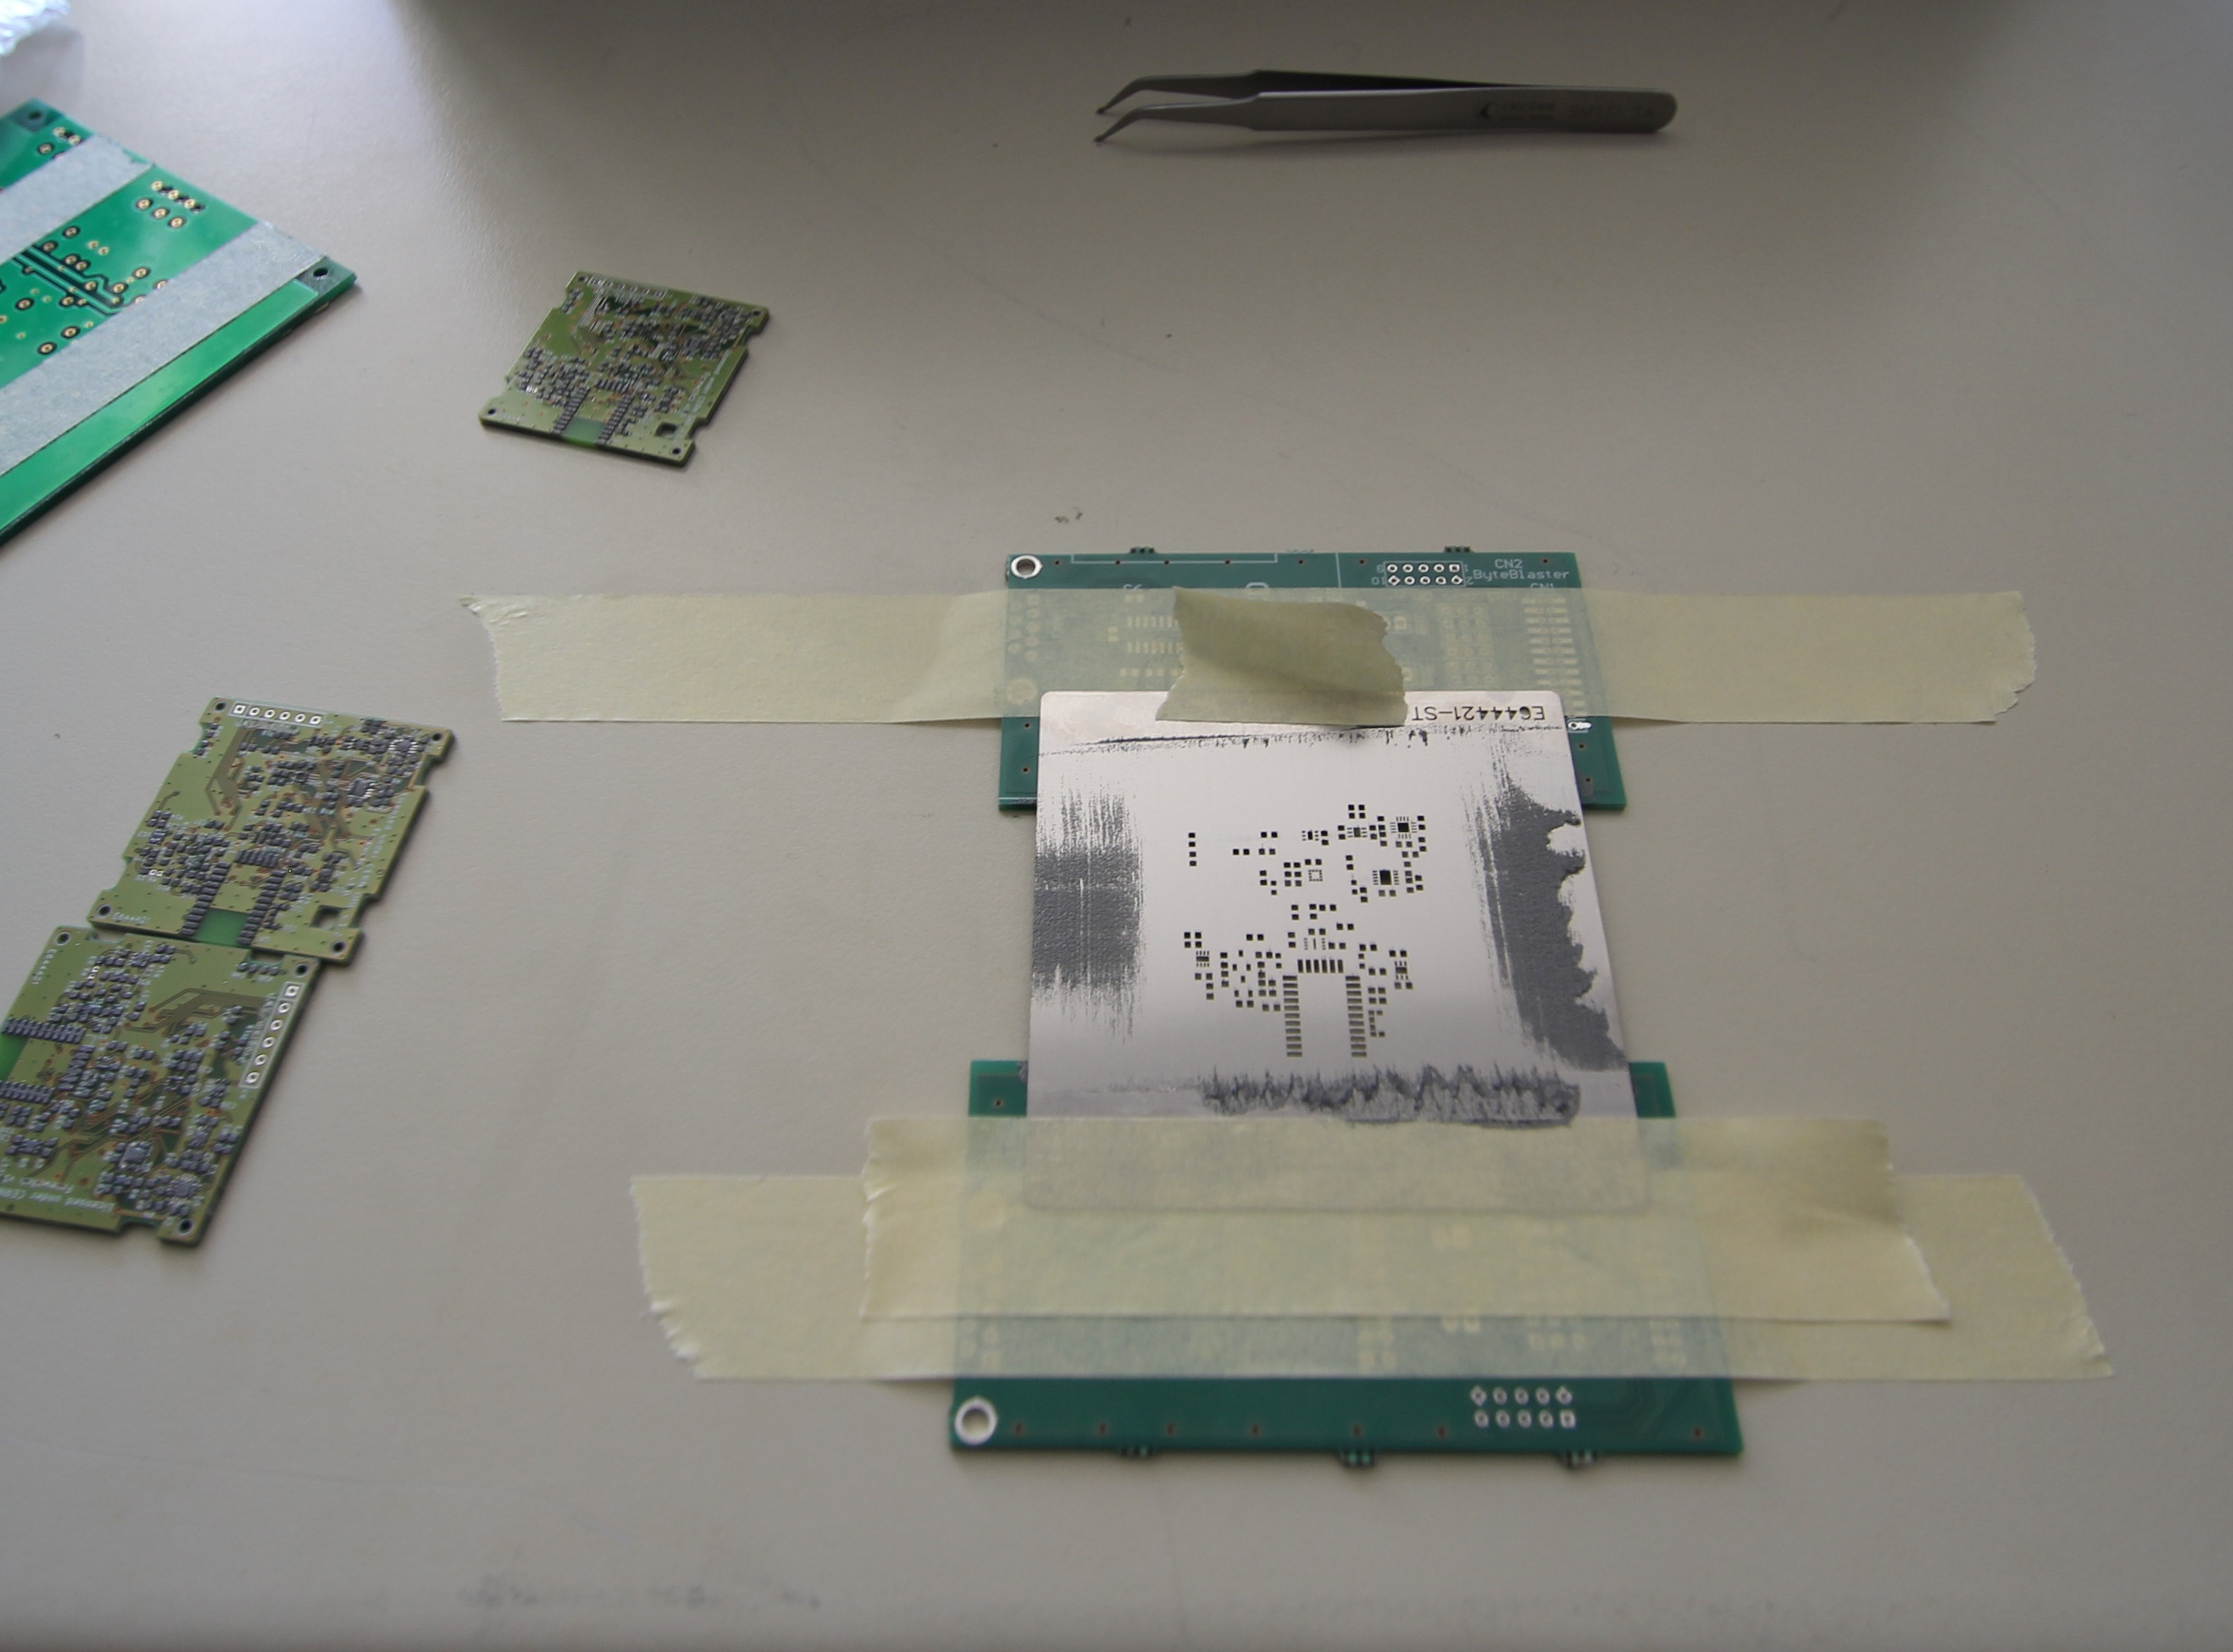
\includegraphics[height=2.5cm]{pcb_stencil_paste.eps}~
    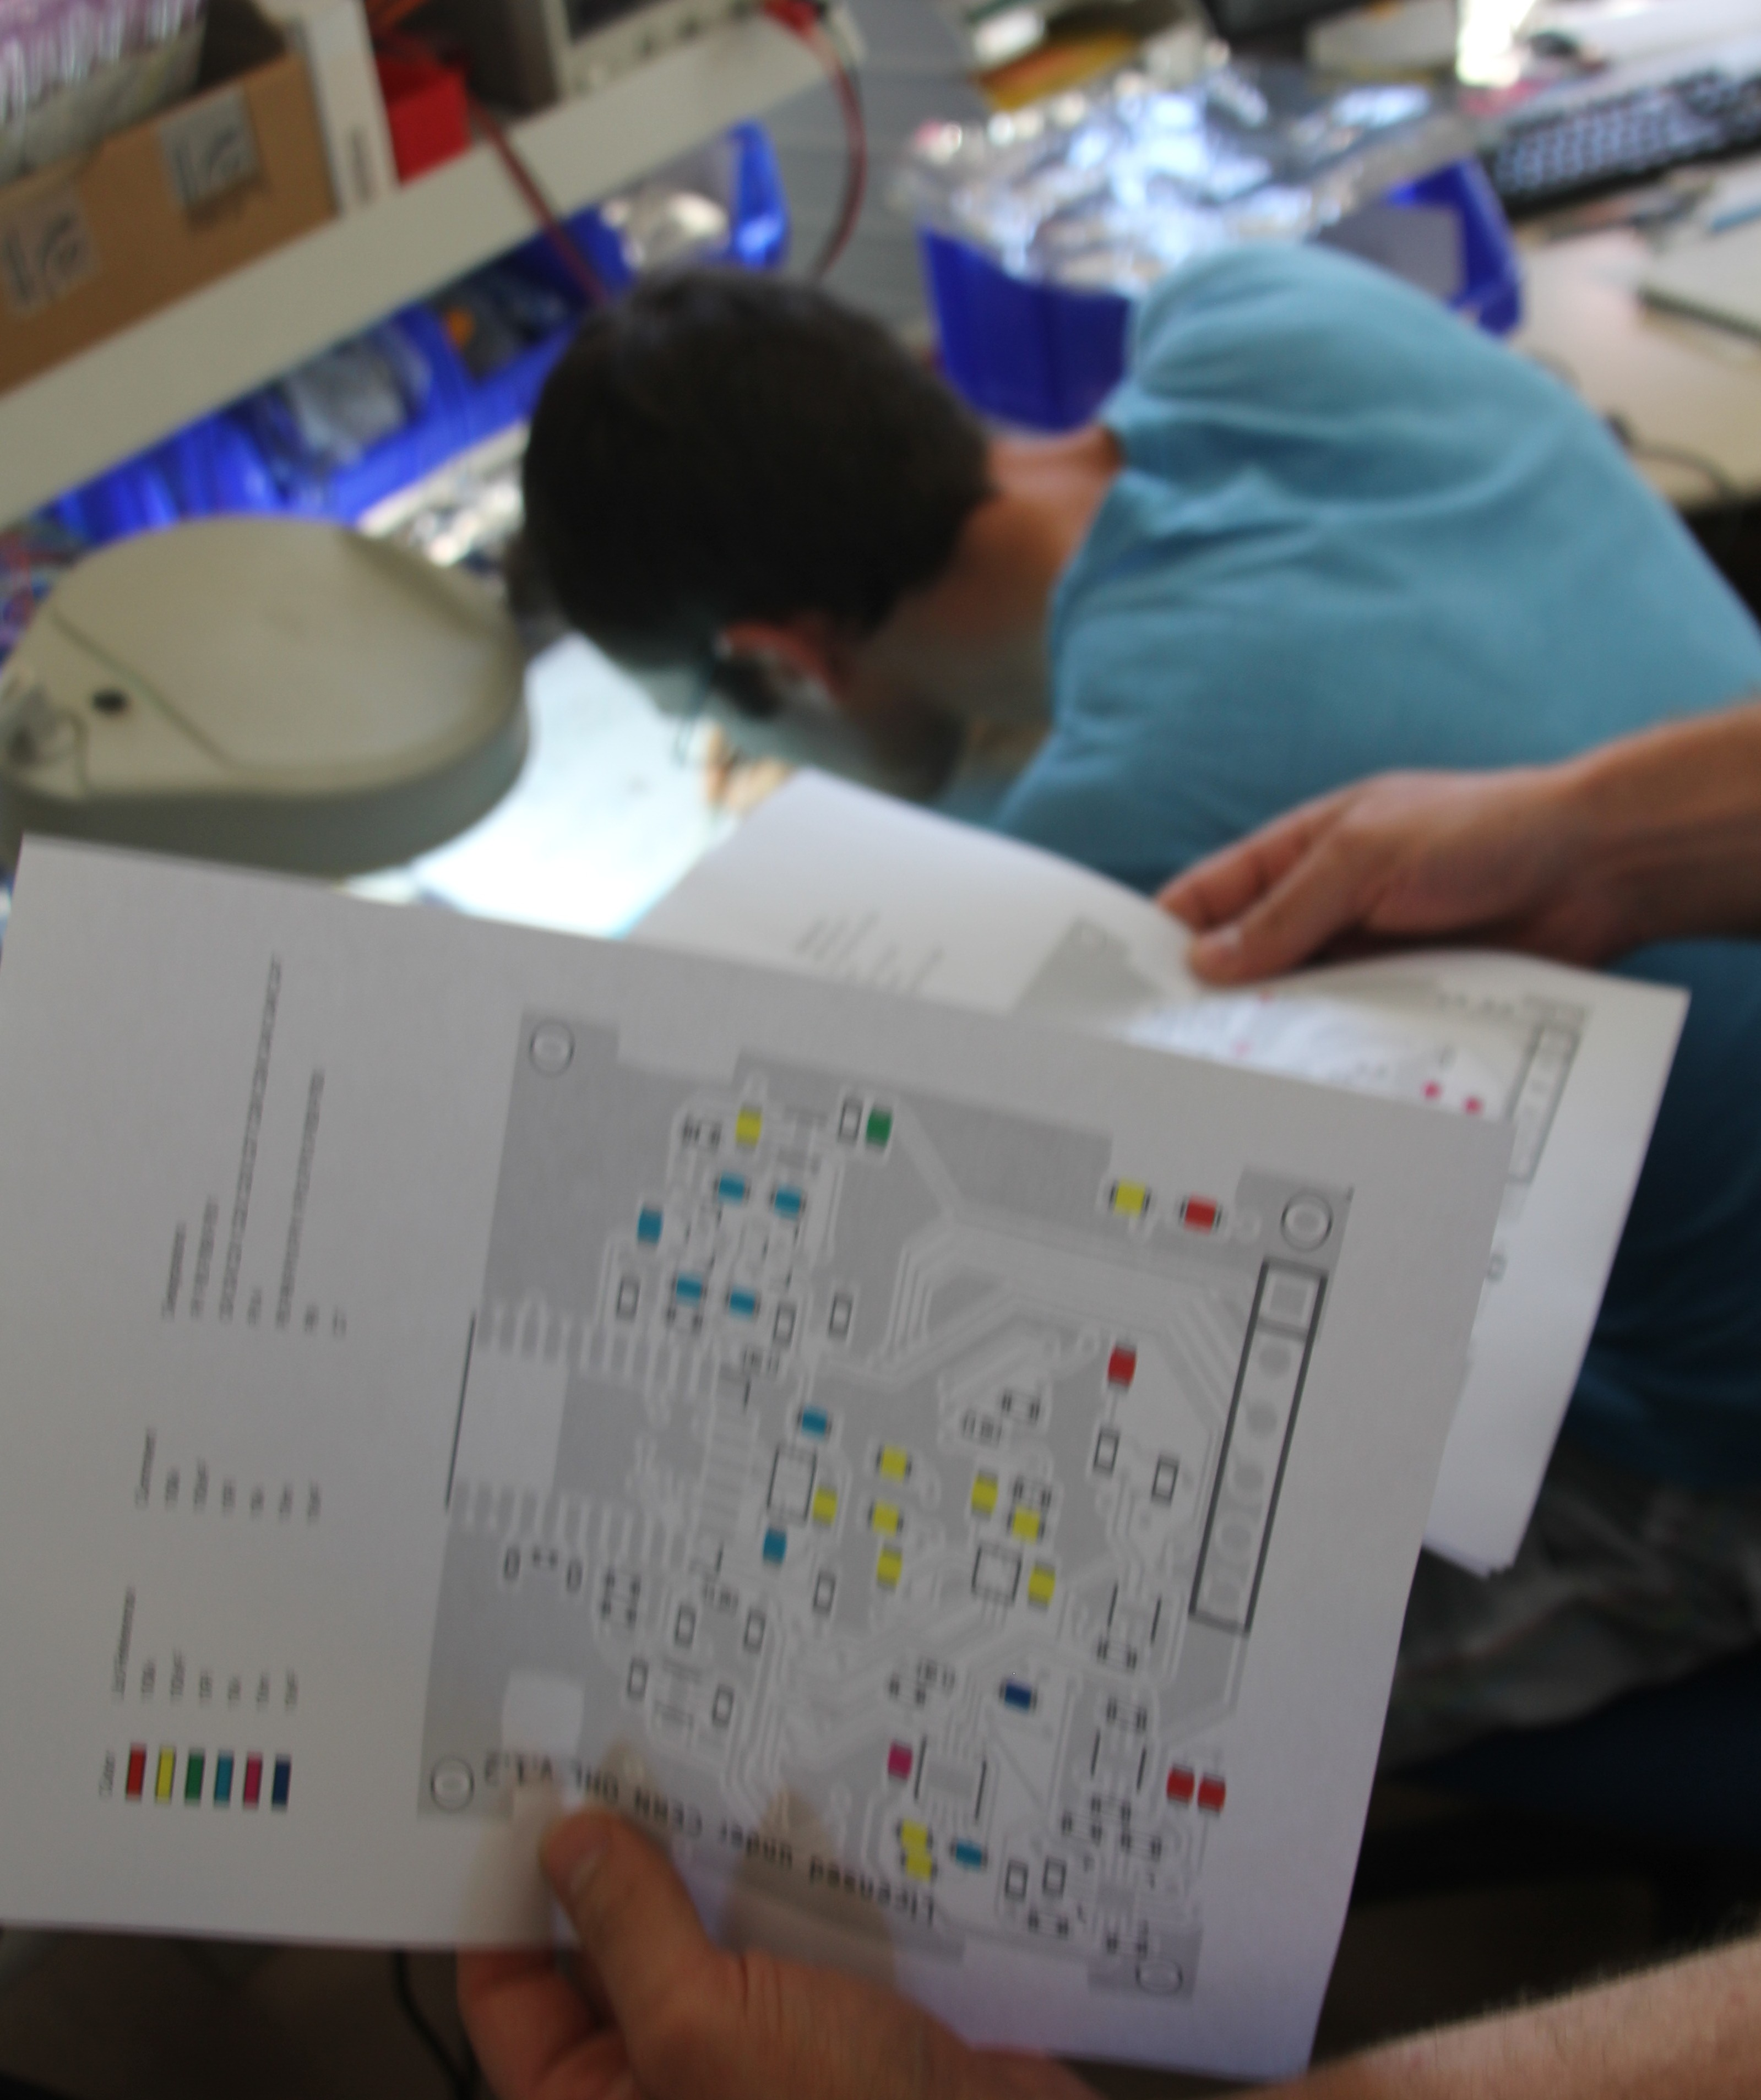
\includegraphics[height=2.5cm]{pcb_assembly_diagram.eps}~
    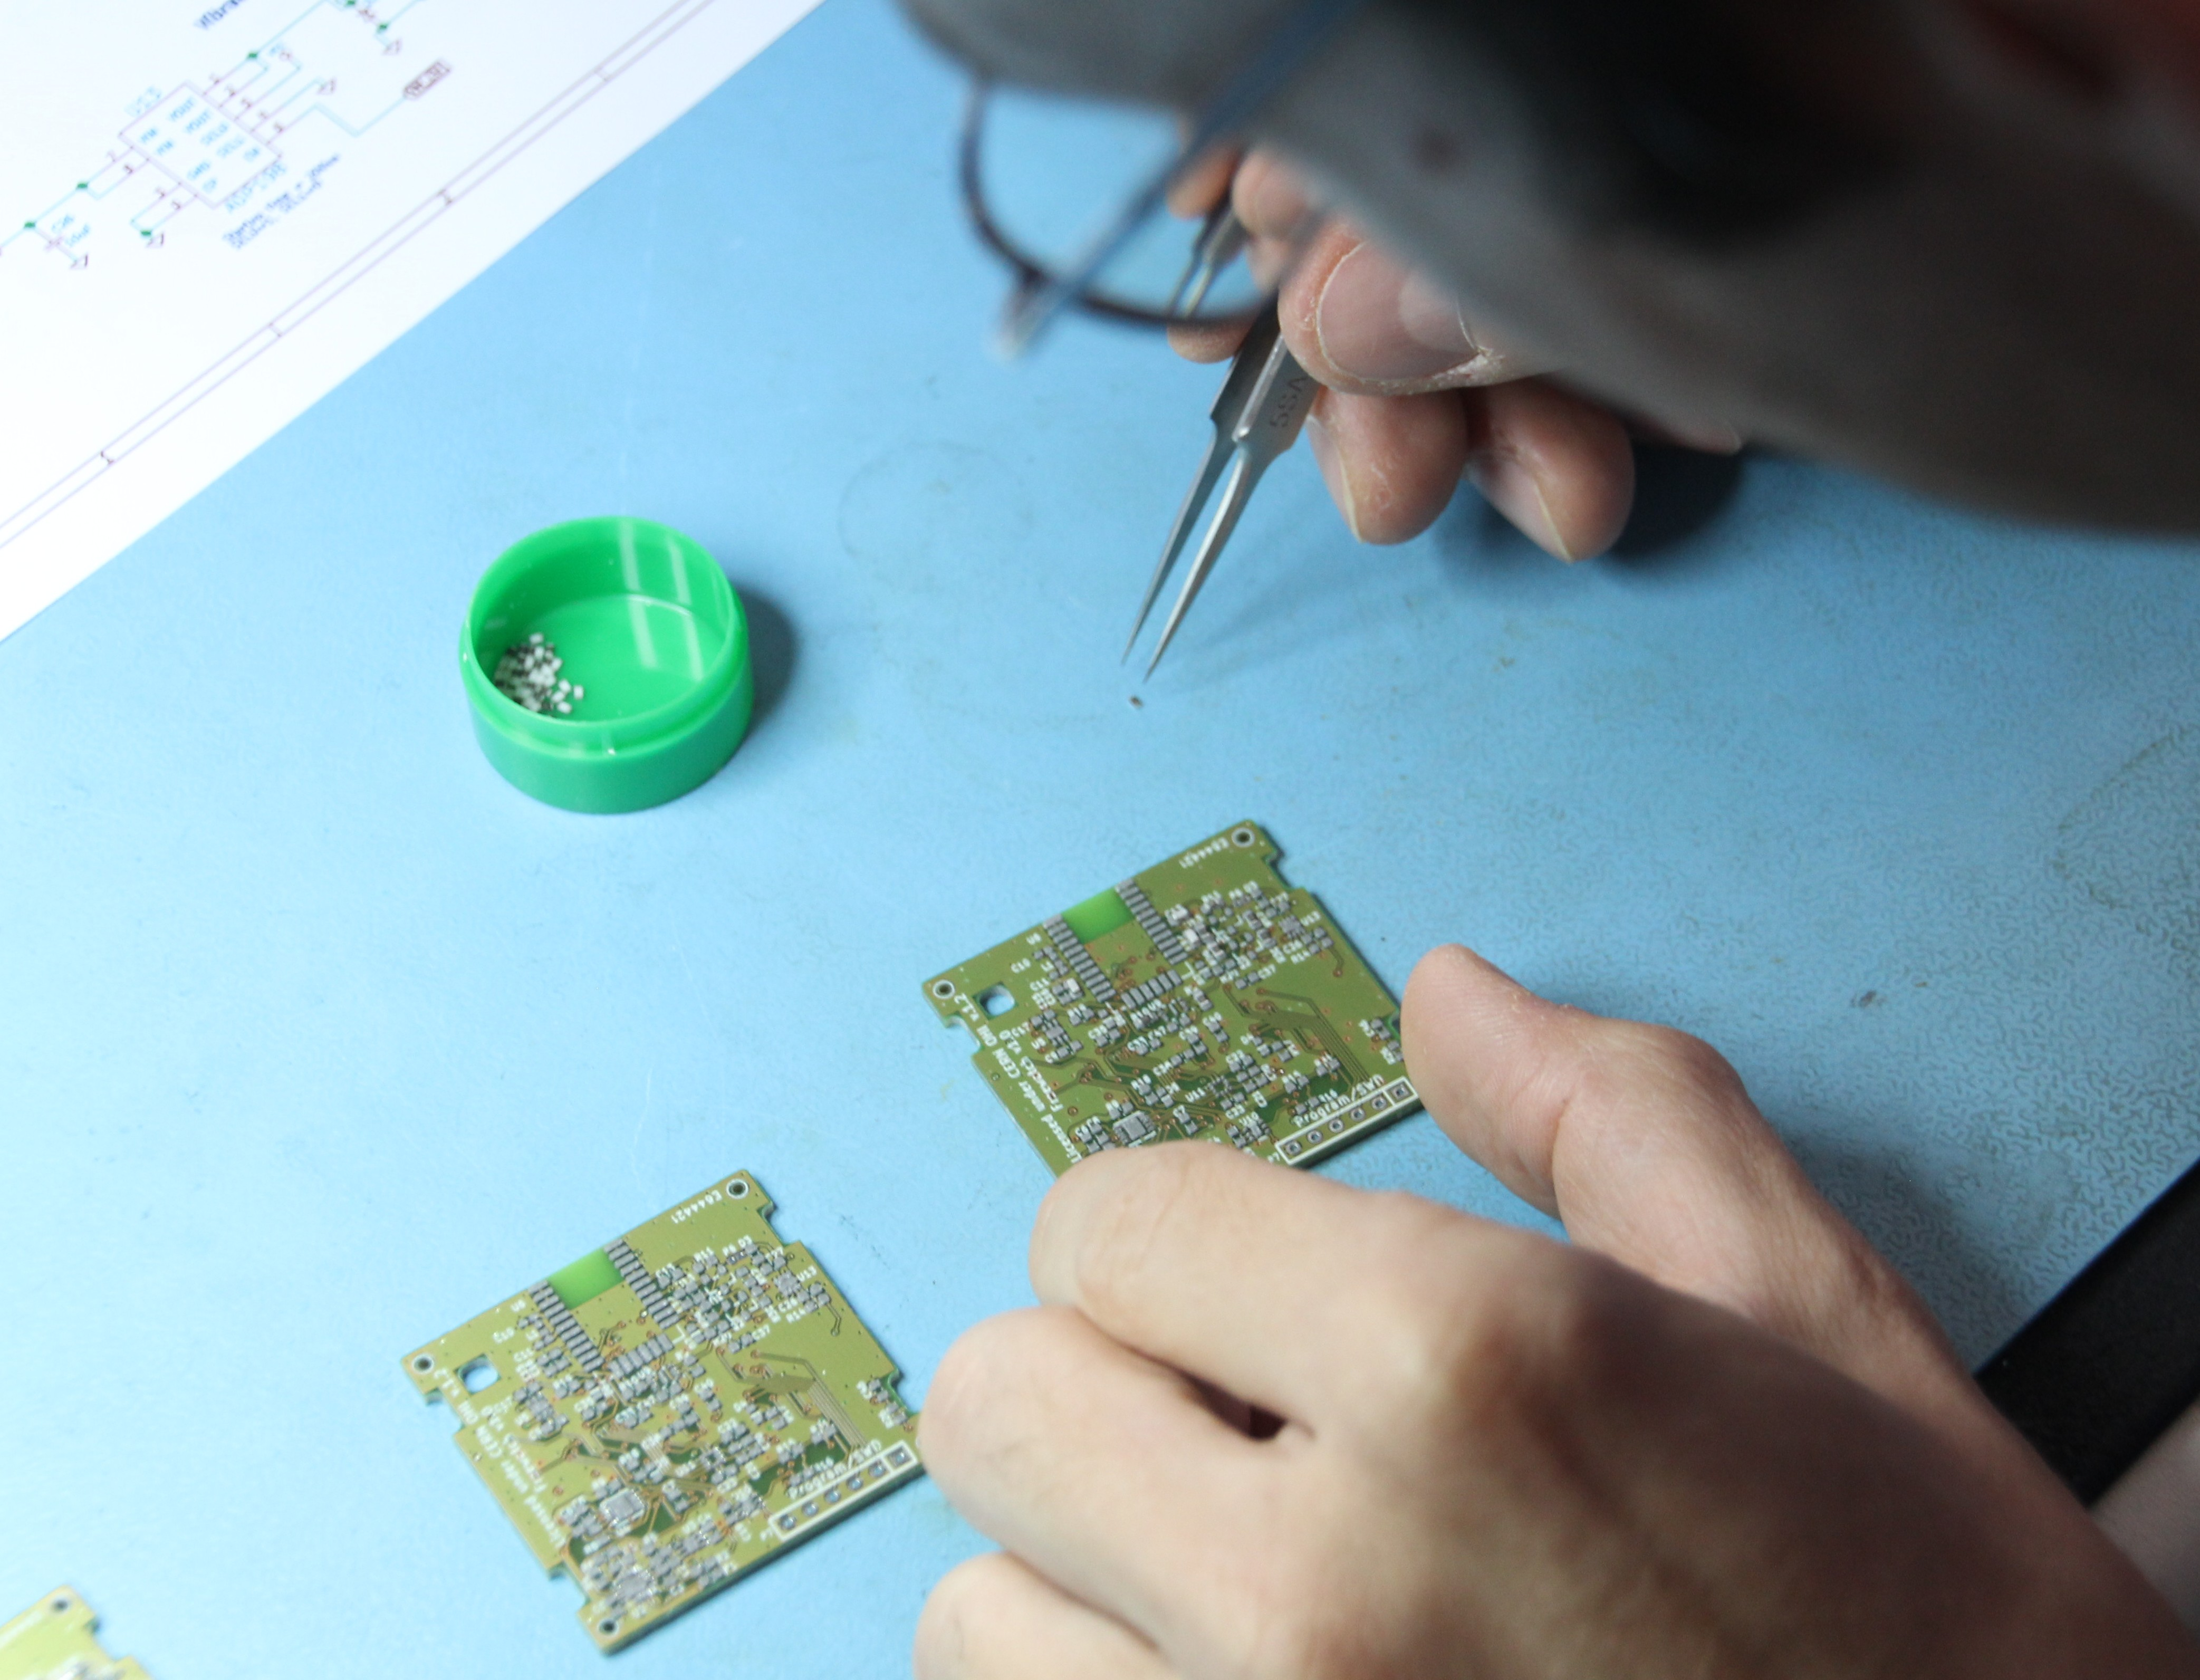
\includegraphics[height=2.5cm]{pcb_component_placement.eps}
  \end{center}

  \note[item]{How we assembled the PCB}
  \note[item]{Stencil needed to solder BGA/QFN components (pins are underneath and not accessible with a soldering iron)}
  \note[item]{Script to generate placement pdf very useful, don't need to go from schematics to layout all the time}
  \note[item]{We don't have an oven for soldering, so we used a hot-air station, which is quite tricky}

\end{frame}

\end{comment}


%------------ FRAME --------------------------------------------------
\begin{frame}{Building the watch}

  Software

  \begin{itemize}
  \item Download sources from the GIT repo
  %\item Find your way through the sources (not nicely bundled, yet)
  \item No binary releases (yet)
  \item Compile bootloader and flash it (using a programmer)
  \item Compile application sw and flash it (using the bootloader)
  \item Modify, re-flash, test, etc...
  \end{itemize}

  \vskip 8mm

  \begin{center}
    \url{git://ohwr.org/f-watch.git}
  \end{center}

  \note[item]{On the software side, it is pretty standard}
  \note[item]{You download the sources from the GIT repository}
  \note[item]{We don't have binary release yet}
  \note[item]{So you will have to compile the bootloader and flash it to the micro-controller using the programmer}
  \note[item]{Then compile the application software and flash it using the bootloader}
  \note[item]{Then you can modify, write your own applications, etc...}
  \note[item]{..[NEXT] cost summary}

\end{frame}

%------------ FRAME --------------------------------------------------
\begin{frame}{How much does it costs?}

  \begin{center}
    \begin{table}[h]
      \begin{tabular}{l|r|r|r|l}
        \cline{2-4}
        & \multicolumn{3}{c|}{Number of watches}                                     &  \\ \cline{2-4}
        & \multicolumn{1}{c|}{1} & \multicolumn{1}{c|}{10} & \multicolumn{1}{c|}{50} &  \\ \cline{1-4}
        \multicolumn{1}{|l|}{Pcb + components}         & 175 \texteuro               & 94 \texteuro                  & 81 \texteuro                  &  \\ \cline{1-4}
        \multicolumn{1}{|l|}{Pcb assembly}             & -                           & 118 \texteuro                 & 67 \texteuro                  &  \\ \cline{1-4}
        \multicolumn{1}{|l|}{Case + buttons + screws}  & 68 \texteuro                & 67 \texteuro                  & 61 \texteuro                  &  \\ \cline{1-4}
        \multicolumn{1}{|l|}{\textbf{TOTAL per watch}} & \textbf{243 \texteuro}      & \textbf{278 \texteuro}        & \textbf{209 \texteuro}        &  \\ \cline{1-4}
        \multicolumn{1}{|l|}{\textbf{TOTAL}}           & \textbf{243 \texteuro}      & \textbf{2'784 \texteuro}      & \textbf{10'455 \texteuro}     &  \\ \cline{1-4}
      \end{tabular}
      \caption{Estimated cost for small series (without shipping)}
    \end{table}
  \end{center}

  %\note[item]{The price in euro are converted from swiss franc with the exchange rate of last week}
  %\note[item]{So it might not be up to date ;)}
  %\note[item]{Review table style to fit Federico's}
  \note[item]{}
  \note[item]{}
  \note[item]{..[NEXT] Federico slide on software}

\end{frame}



\begin{comment}

%#####################################################################
%############ SECTION ################################################
\section{What's next?}

\subsection*{} % dummy subsection to display dots

%------------ FRAME --------------------------------------------------
\begin{frame}{What's next?}

  \begin{block}{Improvements}
    \begin{itemize}
    \item Bluetooth LE
    \item Water-resistance
    \item LCD backlight
    \item Reduce PCB/housing size
    \item 
    \end{itemize}
  \end{block}

  \begin{block}{Software}
    \begin{itemize}
    \item Firmware loader
    \item Data transfer (to/from SD card)
    \item Emulator
    \item Application "ecosystem"
      \begin{itemize}
      \item GPS route following
      \item Atmosheric pressure history
      \item Altitude based on atmospheric pressure
      \item ...
      \end{itemize}
    \end{itemize}
  \end{block}

  \note[item]{}

\end{frame}

%------------ FRAME --------------------------------------------------
\begin{frame}{What's next?}

  \begin{block}{Build a community}
    \begin{itemize}
    \item 
    \item 
    \end{itemize}
  \end{block}
  \note[item]{}

\end{frame}

%------------ FRAME --------------------------------------------------
\begin{frame}{What's next?}

  \begin{block}{Make a kit}
    \begin{itemize}
    \item Pre-assembled PCB option
    \item Customisable strap/housing color
    \item Alternative housing
    \item Sold by a company?
    \end{itemize}
  \end{block}

  \note[item]{}

\end{frame}

\end{comment}



%#####################################################################
%############ SECTION ################################################
\section{Software}

\begin{frame}{MCU SDK}
  \Large
  \begin{center}
    free and open source software \\
    \vskip 1cm
    A lot of integration examples \\
    \vskip 1cm
    Well documented \\
  \end{center}

  \note{Say few things about the SDK}
\end{frame}

%------------ FRAME --------------------------------------------------

\begin{frame}{Bootloader}
  \Large
  \begin{center}
    free bootloader provided by SiliconLab \\
    \vskip 1cm
    support for IAR, Keil uVision \\
    \vskip 1cm
    migrate to gcc toolchain \\
    \vskip 1cm
    (don't use gcc optimization!)
  \end{center}

  \note{Few thing about the bootloader}
\end{frame}

%------------ FRAME --------------------------------------------------

\begin{frame}{Operating System}
 \large
 \begin{center}
  \begin{tabular}{lcccc}
    & FreeRTOS & uC/OS-III & RTX & TNKernel \\[2.5mm]
    \hline
    \\[1mm]
   License & Mod. GPL & restrictive & BSD & BSD \\[5mm]
   EFM32   & yes      & yes         & yes & no  \\[5mm]
   USB     & no       & yes         & no  & yes \\[5mm]
   FAT     & no       & yes         & no  & yes \\
  \end{tabular}
 \end{center}

 \note[item]{raw ordered by importance}
 \note[item]{License main thing}
 \note[item]{uC nice but closed}
 \note[item]{FreeRTOS --- Keil RTX, they don't have FAT and USB}
\end{frame}

%------------ FRAME --------------------------------------------------

\begin{frame}{Operating System}
  \Large
  \begin{columns}[T] % align columns
    \begin{column}{.48\textwidth}
      FreeRTOS
      \vskip 1cm
      \begin{itemize}
      \item nice documentation
        \vskip 1cm
      \item big community
        \vskip 1cm
      \item a lot of examples
      \end{itemize}
    \end{column}
    \hfill%
    \begin{column}{.48\textwidth}
      Keil RTX
      \vskip 1cm
      \begin{itemize}
      \item nice documentation
        \vskip 1cm
      \item community?
        \vskip 1cm
      \item few examples
      \end{itemize}
    \end{column}%
  \end{columns}

  \note[item]{The main criterium here was the level of knowledge sharing
    around the projects}
  \note[item]{The choice is done, but I'm personally curious so if you know
    where it is the community around RTX (forum, irc channel, blog)
    let me know. }
\end{frame}

%------------ FRAME --------------------------------------------------
\begin{frame}{Graphic}
  \Large
  \begin{center}
    tiny 2D graphic library \\
    \vskip 7mm
    adapt the library to our screen \\
  \end{center}

  \vskip 7mm
  \textbf{Features}
  \vskip 4mm

  \begin{itemize}
  \item write text
    \vskip 4mm
  \item draw simple geometry and icons
    \vskip 4mm
  \item event management
  \end{itemize}

  \note[item]{Internally, one of us already wrote a tiny graphic library}
  \note[item]{we adapted the library to our screen}
  \note[item]{The library allows to write text of different size}
  \note[item]{it allows to draw simple geometries like: line, triangles,
    rectangles, circles, and icons}
  \note[item]{Graphic element can act on event}
\end{frame}

%------------ FRAME --------------------------------------------------

\begin{frame}{Applications}
  \begin{center}
    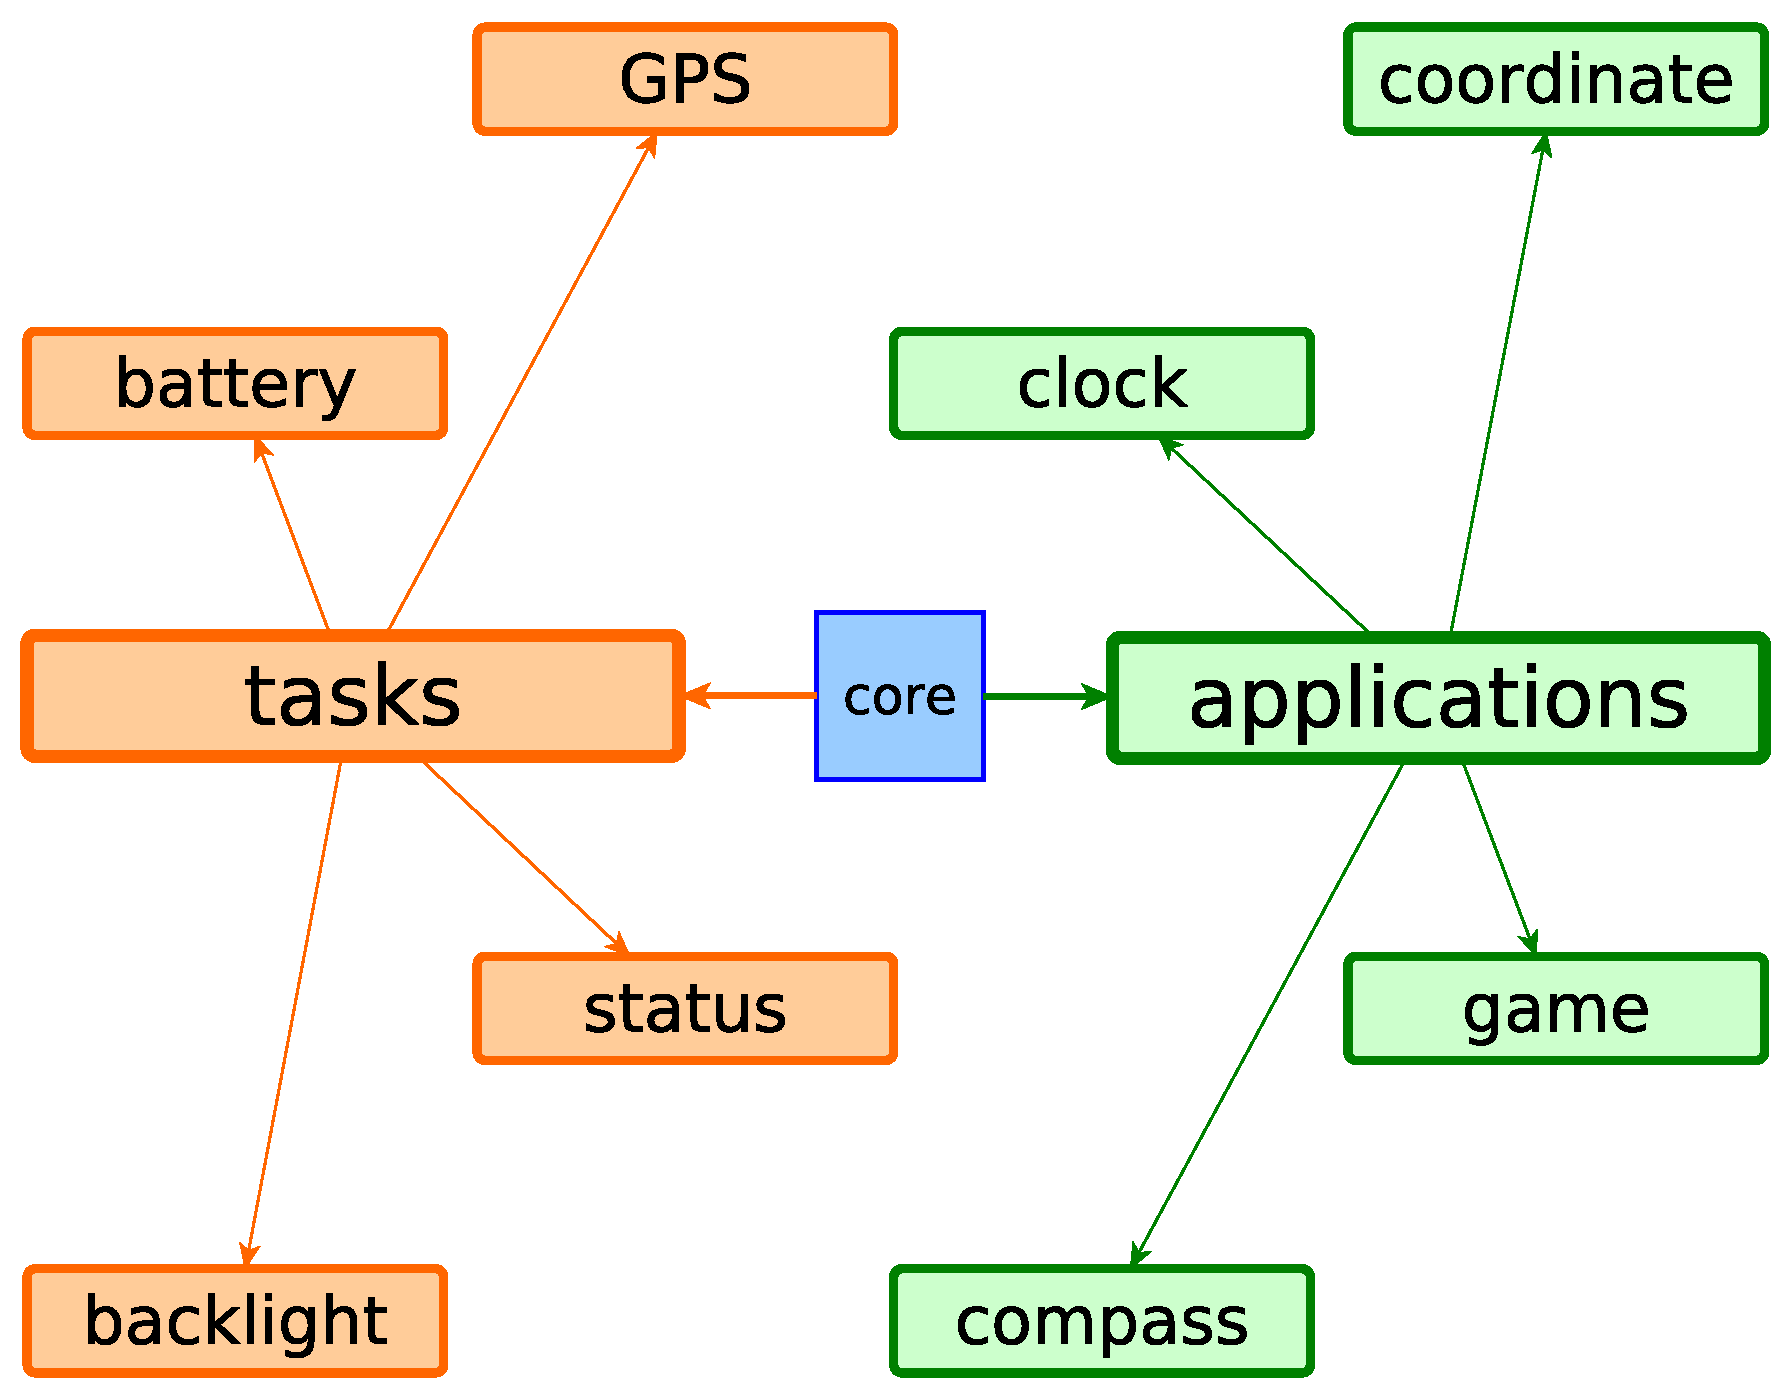
\includegraphics[height=7cm]{sw-app.eps}
  \end{center}

  \note{DO NOT SAY TOO MUCH, THERE WILL BE THE VIDEO LATER}
  \note[item]{drivers behind}
  \note[item]{task: say basically what they do}
  \note[item]{GPS - time, tracking if enable}
  \note[item]{apps: say basically what they do}
\end{frame}

%------------ FRAME --------------------------------------------------
\begin{frame}{Interface}
  \begin{center}
    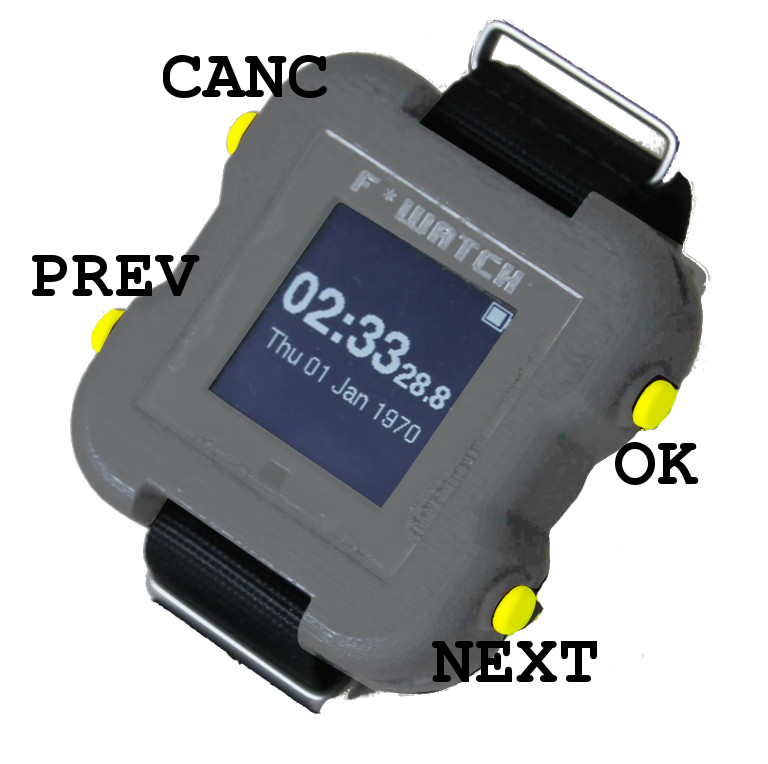
\includegraphics[height=7.5cm]{fwatch-full-side-btn.eps}
  \end{center}
\end{frame}

\begin{frame}{Demo}
  \begin{center}
    \begin{figure}[h!]
      \centering
      \movie[height=5cm, width = 5cm, autostart, once, showcontrols=true,
        borderwidth=1pt, poster]{Applications Demonstration}{../video/fosdemlow.mp4}
    \end{figure}
  \end{center}
  \note{just comment the video. The menu easy to configue thanks to a config
    structure}
\end{frame}

%------------ FRAME --------------------------------------------------

\begin{frame}{Documentation}
  \Large
  \begin{center}
      www.ohwr.org/projects/f-watch/wiki
  \end{center}
  \vskip 1cm
  \begin{itemize}
  \item how to configure your machine
    \vskip 7mm
  \item how to write applications
    \vskip 7mm
  \item details about the project
  \end{itemize}

  \note{Few words about the project documentation}
\end{frame}

%#####################################################################
%############ SECTION ################################################
\section{Conclusions}

\begin{frame}{Development Summary}
  \Large
  \begin{columns}[T] % align columns
    \begin{column}{.55\textwidth}
      \begin{itemize}
      \item free PCB design
        \vskip 8mm
      \item free mechanic design
        \vskip 8mm
      \item free software
        \vskip 8mm
       \item free tools
      \end{itemize}
        \note[item]{just read list}
        \note[item]{Free Tools --- This is madness! --- Madness? This
          is Free Development!}
    \end{column}
    \hfill%
    \pause
    \begin{column}{.43\textwidth}
      \vskip 18mm
      \begin{center}
        \textbf{free} development \\
        for\\
        \textbf{free} products
      \end{center}
        \note[item]{A lot of good free tools for sw devel}
        \note[item]{free tools often crappy}
        \note[item]{fortunatelly today some of them are mature and
          competitive}
    \end{column}%
  \end{columns}
\end{frame}

%------------ FRAME --------------------------------------------------

\begin{frame}{Free Development Needs Free Tools}
  \begin{center}
    \alt<2> {
      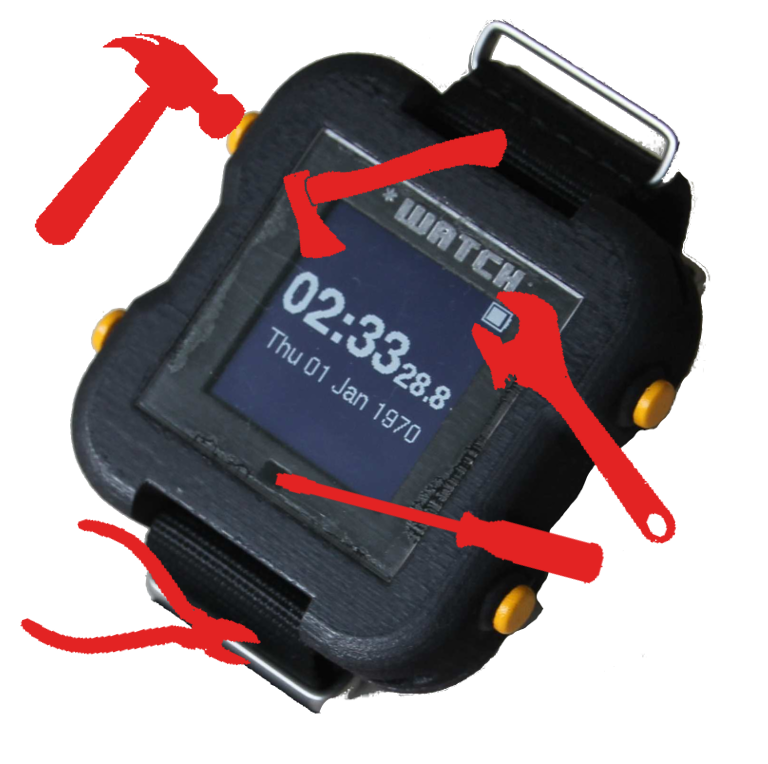
\includegraphics[height=7.5cm]{fwatch-full-side-tool.eps}
    }{
      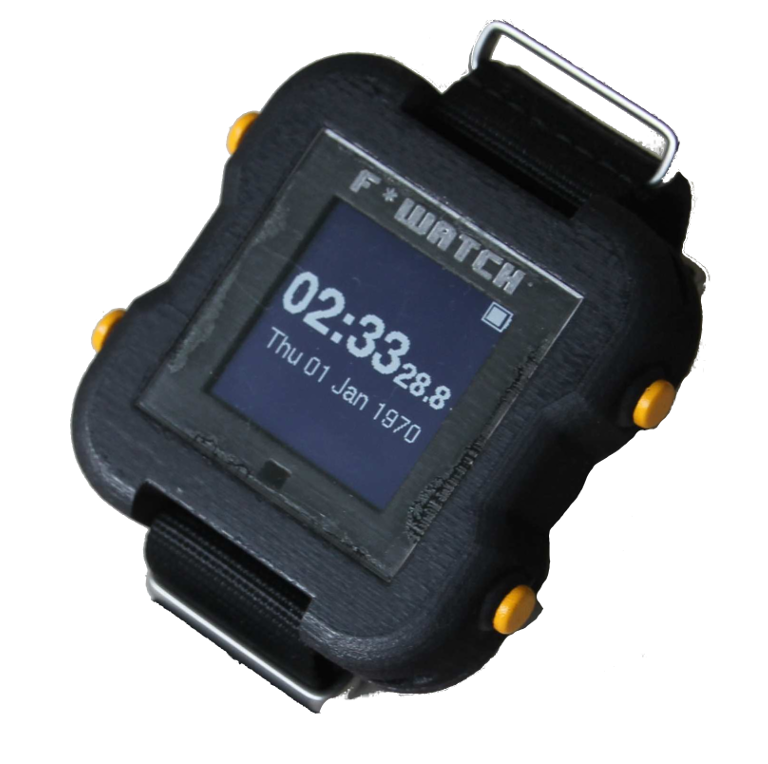
\includegraphics[height=7.5cm]{fwatch-full-side.eps}
    }
  \end{center}

  \note[item]{Software is really easy to share}
  \note[item]{Hardware sharing depends on tool and file format ---}

  \note[item]{The first consideration. For a free development we
    absolutely need free file format and tools to ease sharing}
  \note[item]{.doc MS office example}
  \note[item]{it was a pain}
  \note[item]{today, comparable}
  \note[item]{CERN experience}
\end{frame}

%------------ FRAME --------------------------------------------------

\begin{frame}{Easy to Make}
  \Large
  \begin{center}
    How difficult can be? \\
    \vskip 1cm
    Competitive free tools \\
    \vskip 1cm
    Specialized company in 3D printing \\
    \vskip 1cm
    Specialized company in PCB manufacturing \\
    \vskip 1cm
    Easy to ship everywhere
 \end{center}

  \note[item]{The second consideration is that today is so easy the
    step from the idea to product}
\end{frame}

%------------ FRAME --------------------------------------------------

\begin{frame}{Next Generation Free-Open Source}
  \Large
  \begin{center}
    Free product are real \\
    \vskip 1cm
    cars, robots, watches, bikes, houses, phones, ... \\
    \vskip 1cm
    3D Metal printers \\
  \end{center}

  \note[item]{Open source movement is growing as usual}
  \note[item]{Open source is every where, different areas}
  \note[item]{People are starting to use free tools}
  \note[item]{3D metal printer are going to accelerate this expansion}
\end{frame}

%------------ FRAME --------------------------------------------------

\begin{frame}{What can it be?}
  \vskip -5mm
  \begin{columns}[T] % align columns
    \begin{column}{.48\textwidth}
      \begin{center}
        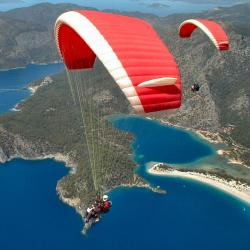
\includegraphics[height=3.5cm]{fwatch-para.eps} \\
        \vskip 5mm
        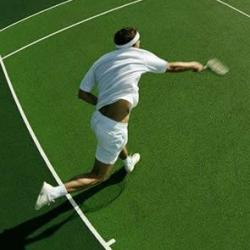
\includegraphics[height=3.5cm]{fwatch-tenn.eps}
      \end{center}
    \end{column}
    \hfill%
    \begin{column}{.48\textwidth}
      \begin{center}
        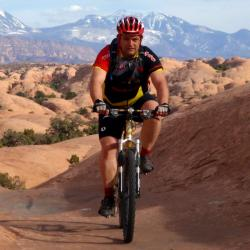
\includegraphics[height=3.5cm]{fwatch-bike.eps} \\
        \vskip 5mm
        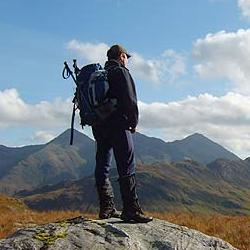
\includegraphics[height=3.5cm]{fwatch-trek.eps}
      \end{center}
    \end{column}%
  \end{columns}

  \note[item]{paraglaiding - accelerometer, compass, pressure, GPS position}
  \note[item]{tennis - acceleromenter, compass - track arm movements}
  \note[item]{bike - GPS position, speed calculation, accelerometer}
  \note[item]{trekking - GPS position, altitude}
\end{frame}

%------------ FRAME --------------------------------------------------

\begin{frame}{Join Us}
  \Large
  \begin{center}
    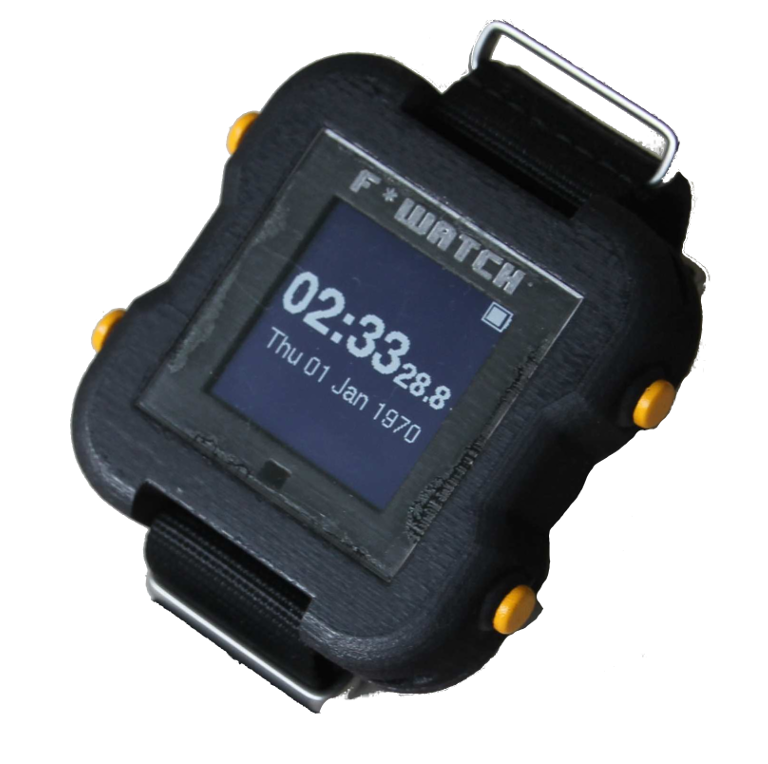
\includegraphics[height=3.5cm]{fwatch-full-side.eps} \\
    \vskip 5mm
    Not a real product \\
    \vskip 5mm
    Make it a good example \\
    \vskip 5mm
    Join the project \\
  \end{center}

  \note[item]{not a real product}
  \note[item]{it would be good to have a mechanical expert}
  \note[item]{company can do it better}
  \note[item]{in general join the project}
  \note[item]{make it a good example}
\end{frame}


\begin{comment}
\end{comment}


\end{document}


